\section{Estimation of the Standard Model Backgrounds}
\label{sec:hh_background_estimate}

%%%%%%%%%%%%%%%%%%%%%%%%%%%%%%%%%%%%%%%%%%%%%%%%%%%%%%%%%%%%%%%%%%%%%%%%%%%%%%%%%%%
%%%%%%%%%%%%%%%%%%%%%%%%%%%%%%%%%%%%%%%%%%%%%%%%%%%%%%%%%%%%%%%%%%%%%%%%%%%%%%%%%%%
%%%%%%%%%%%%%%%%%%%%%%%%%%%%%%%%%%%%%%%%%%%%%%%%%%%%%%%%%%%%%%%%%%%%%%%%%%%%%%%%%%%
%
% TOP QUARK BACKGROUNDS
%
%%%%%%%%%%%%%%%%%%%%%%%%%%%%%%%%%%%%%%%%%%%%%%%%%%%%%%%%%%%%%%%%%%%%%%%%%%%%%%%%%%%
%%%%%%%%%%%%%%%%%%%%%%%%%%%%%%%%%%%%%%%%%%%%%%%%%%%%%%%%%%%%%%%%%%%%%%%%%%%%%%%%%%%
%%%%%%%%%%%%%%%%%%%%%%%%%%%%%%%%%%%%%%%%%%%%%%%%%%%%%%%%%%%%%%%%%%%%%%%%%%%%%%%%%%%

\FloatBarrier
\subsection{Top Quark Backgrounds}
\label{sec:cr_top}

We define a CR for the SM background that composed of the sum of the \ttbar~and single-top $Wt$
process, referred to simply as the Top background.
In reality, already at NLO, these two processes become difficult to distinguish between one another
due to their leading both to the $WbWb$ final state with interfering diagrams.
These interference effects are not properly accounted for in the MC simulation.
This ambiguity in their separate definition is the motivating reason for combining them into a single
process `Top' and treating their sum as a single process, since this is how they behave in data.
Towards this aim, we define CR-Top to provide a data-driven normalization correction on the combined Top
background.
The aim of CR-Top is to provide a correction to the Top background that is representative of that in the SRs
defined in Table~\ref{tab:hh_sr_def}.
For this to be the case, CR-Top is defined so that the Top background composition is very similar to that
found in the SRs.
That is, the relative proportion of the simulated \ttbar~and single-top $Wt$ in the Top background appearing
in SR-SF and SR-DF is the same as that appearing in the Top background in CR-Top.
In this way, the normalisation correction will correct for any interference effects not properly accounted for
in the MC simulation.

The definition of the associated CR and VR, CR-Top and VR-Top, are given in Table~\ref{tab:hh_crtop}.
As with CR-Top, VR-Top is defined to have similar Top background composition as the SRs.
CR-Top and VR-Top select DF and SF events, respectively.
Given that the Top background is flavor symmetric, this is an appropriate extrapolation to make.
Both CR-Top and VR-Top are defined to be orthogonal to the SR selections by inverting the Higgs mass requirement
defined by the $m_{bb}$ observable.
For CR-Top, the $m_{bb}$ requirements are inverted entirely, while for VR-Top only the upper portion of the $m_{bb}$
distribution is selected since, in the SF dilepton events, the lower tail of $m_{bb}$ is contaminated by $Z$-boson
processes.
The \dhh requirements, relative to those in the SRs, are relaxed so as to increase the available statistics.

Figures~\ref{fig:crtop_kin_plots_0}-\ref{fig:crtop_kin_plots_2} show distributions of the relevant
observables in CR-Top.
Figure~\ref{fig:crtop_nm1_dhh} shows the distribution of the composite discriminant \dhh in CR-Top
without the requirement on \dhh applied, so that the full shape of the discriminant may be studied.

\begin{table}[!htb]
    \begin{center}
        \caption{
            Definitions of the CR and VR for the Top quark backgrounds (\ttbar~and single-top $Wt$)
            for the search targeting the dilepton $hh \rightarrow \bbww$ process.
        }
        \label{tab:hh_crtop}
        \begin{tabular}{l | c c}
        \hline
        \hline
                & \multicolumn{2}{c}{\textbf{Region}} \\
            \cline{2-3}
            \textbf{Observable} & \textbf{CR-Top} & \textbf{VR-Top} \\
            \hline
            Dilepton Flavor & $e\mu$ or $\mu e$ & $ee$ or $\mu \mu$ \\
            $b$-tagged jet multiplicity & $\ge 2$ & $\ge 2$ \\
            $m_{bb}$ [GeV] & $<100$ or $>140$ & $>140$ \\
            $m_{\ell \ell}$ [GeV] & $<60$ & $<60$ \\
            \dhh & $>4.5$ & $>4.5$ \\
        \hline
        \hline
        \end{tabular}
    \end{center}
\end{table}

\begin{figure}[!htb]
    \centering
    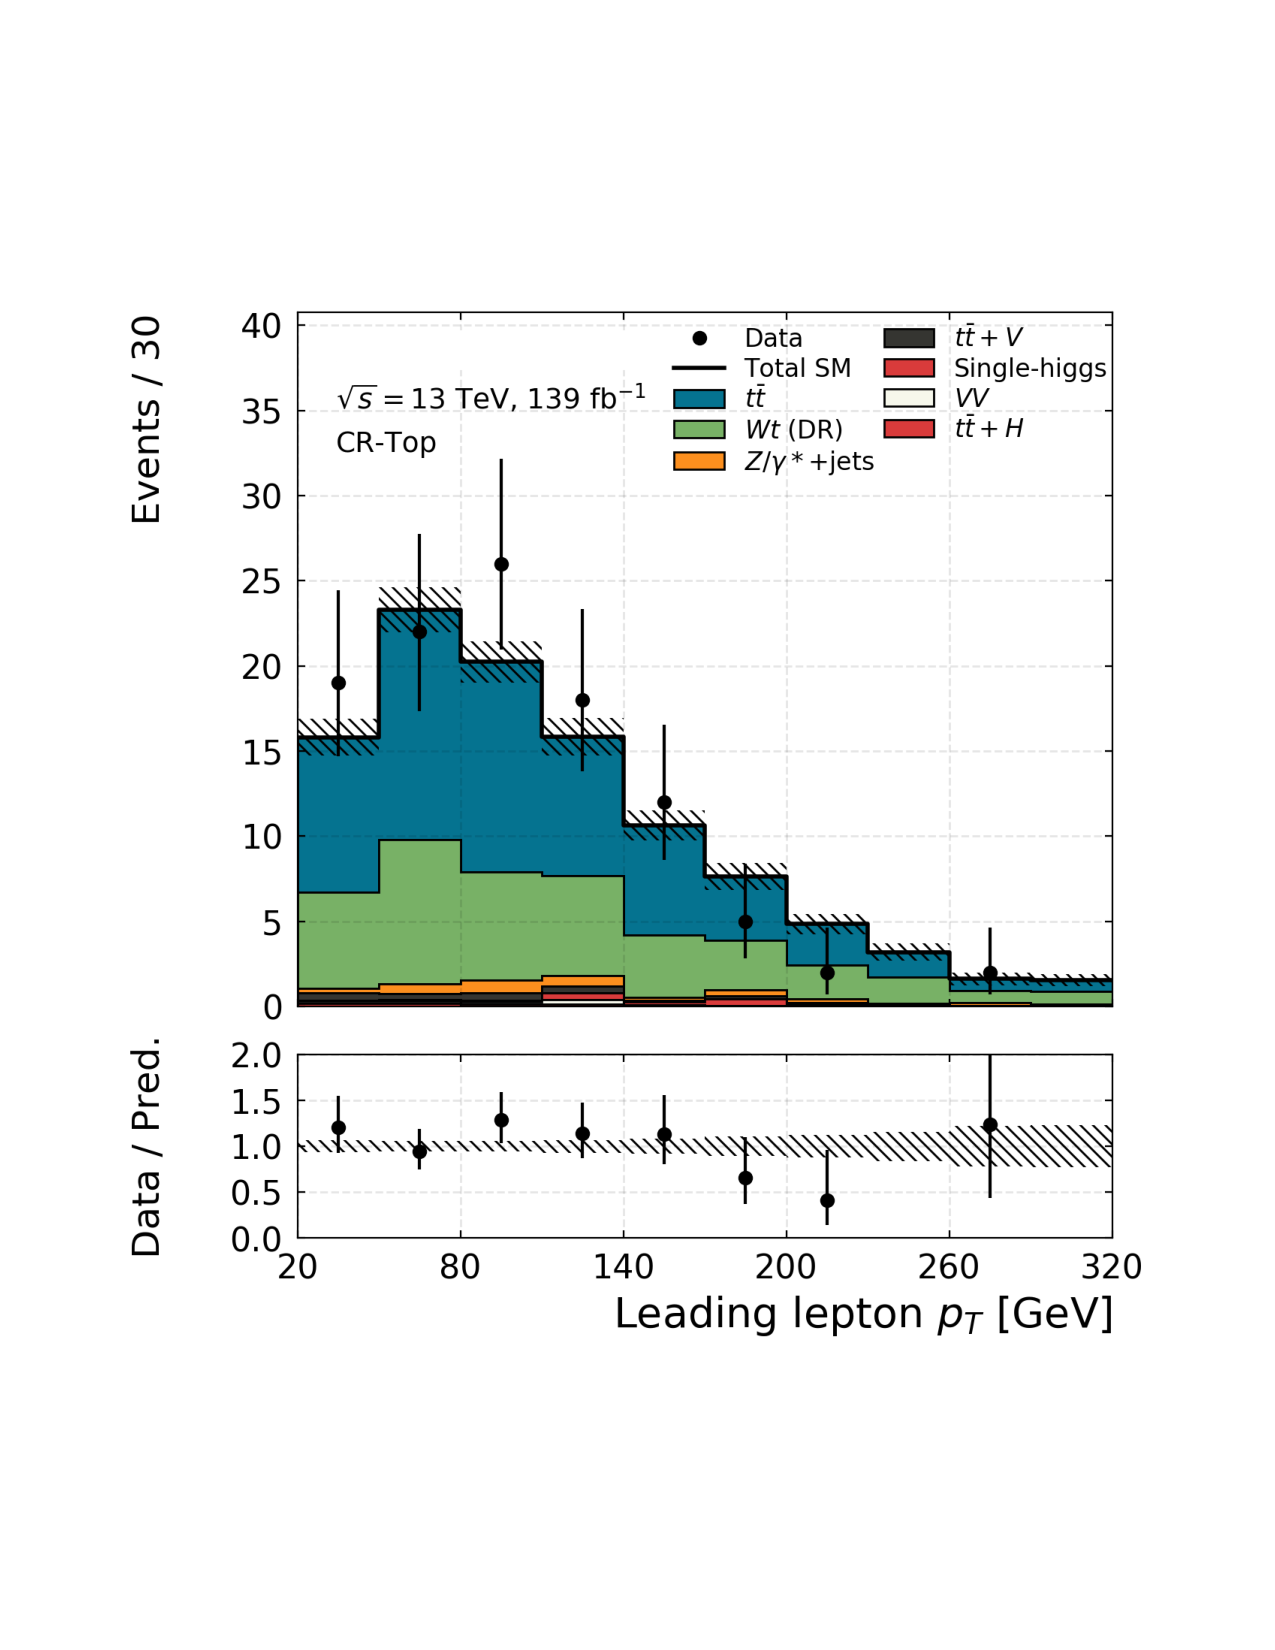
\includegraphics[width=0.4\textwidth]{figures/search_hh/bkg_estimate/crvr/crtop/crtoptest_l0_pt}
    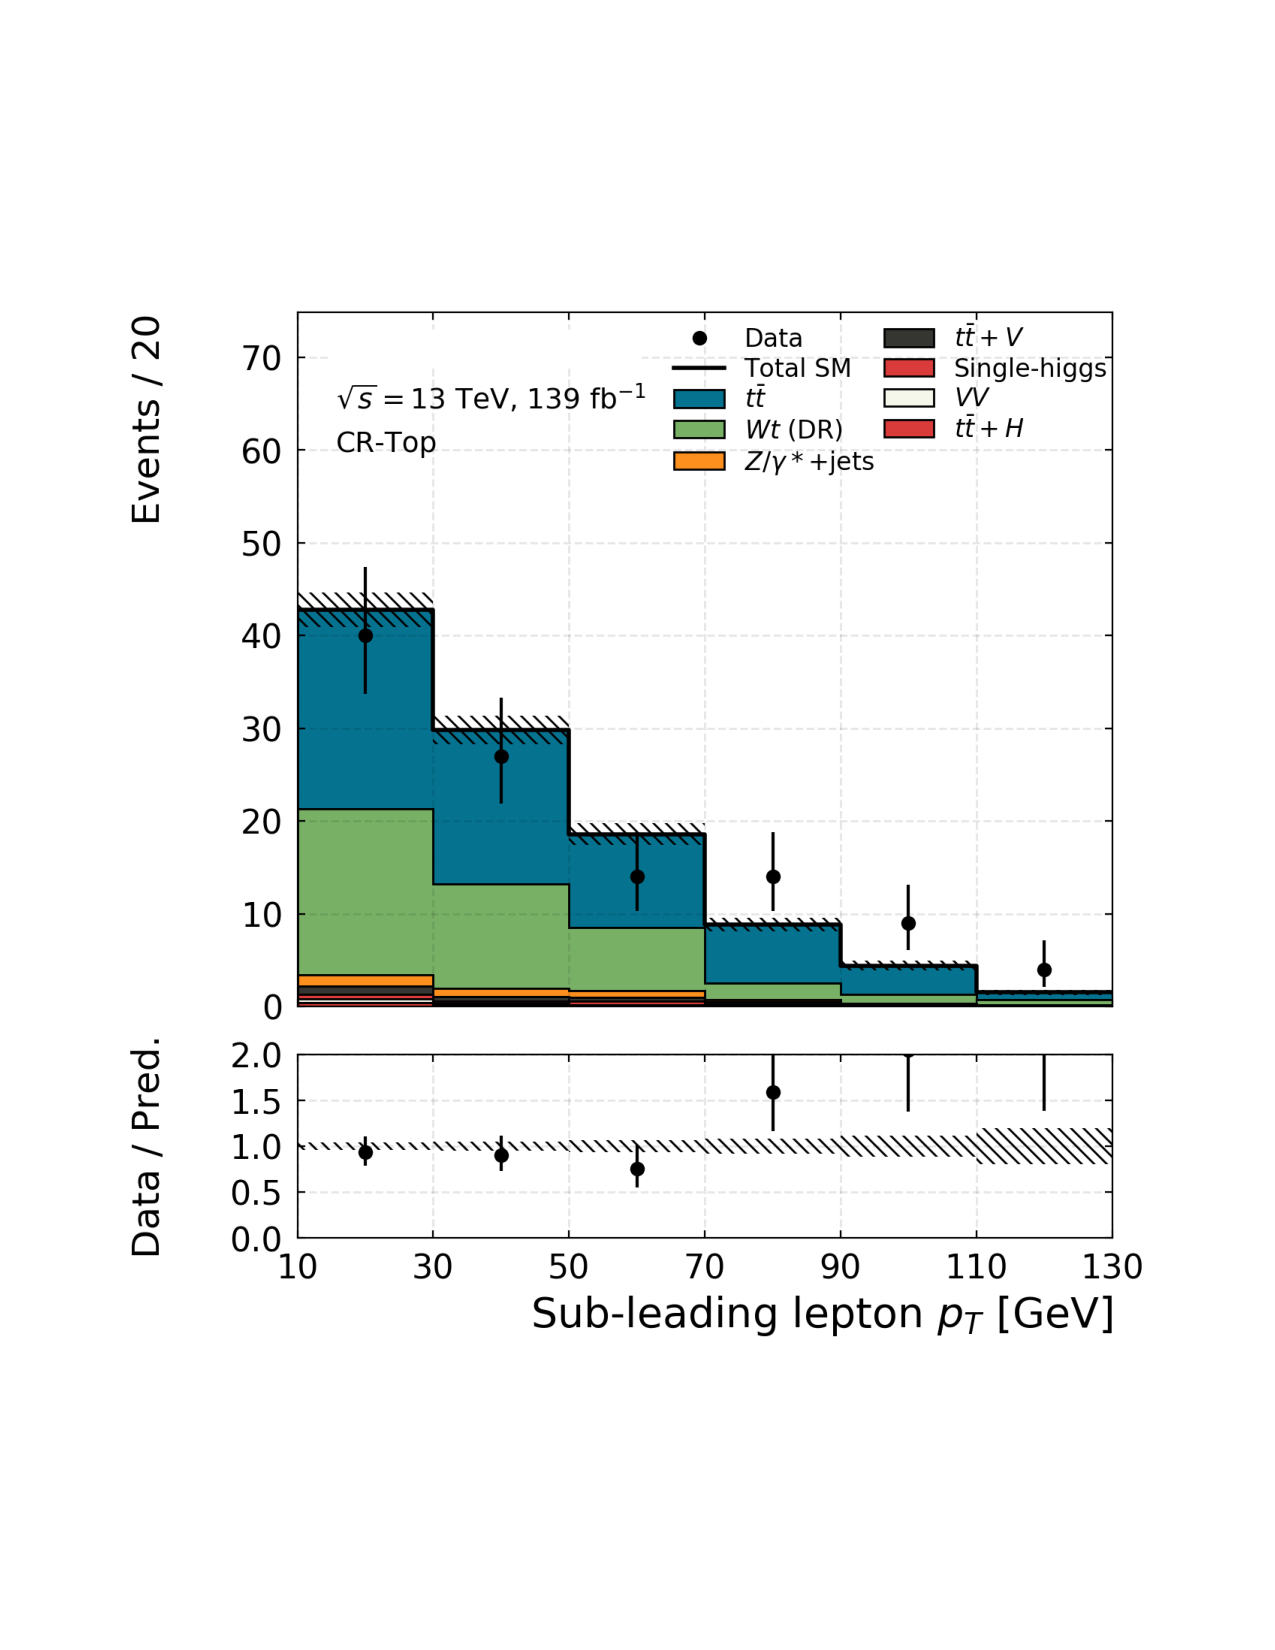
\includegraphics[width=0.4\textwidth]{figures/search_hh/bkg_estimate/crvr/crtop/crtoptest_l1_pt}
    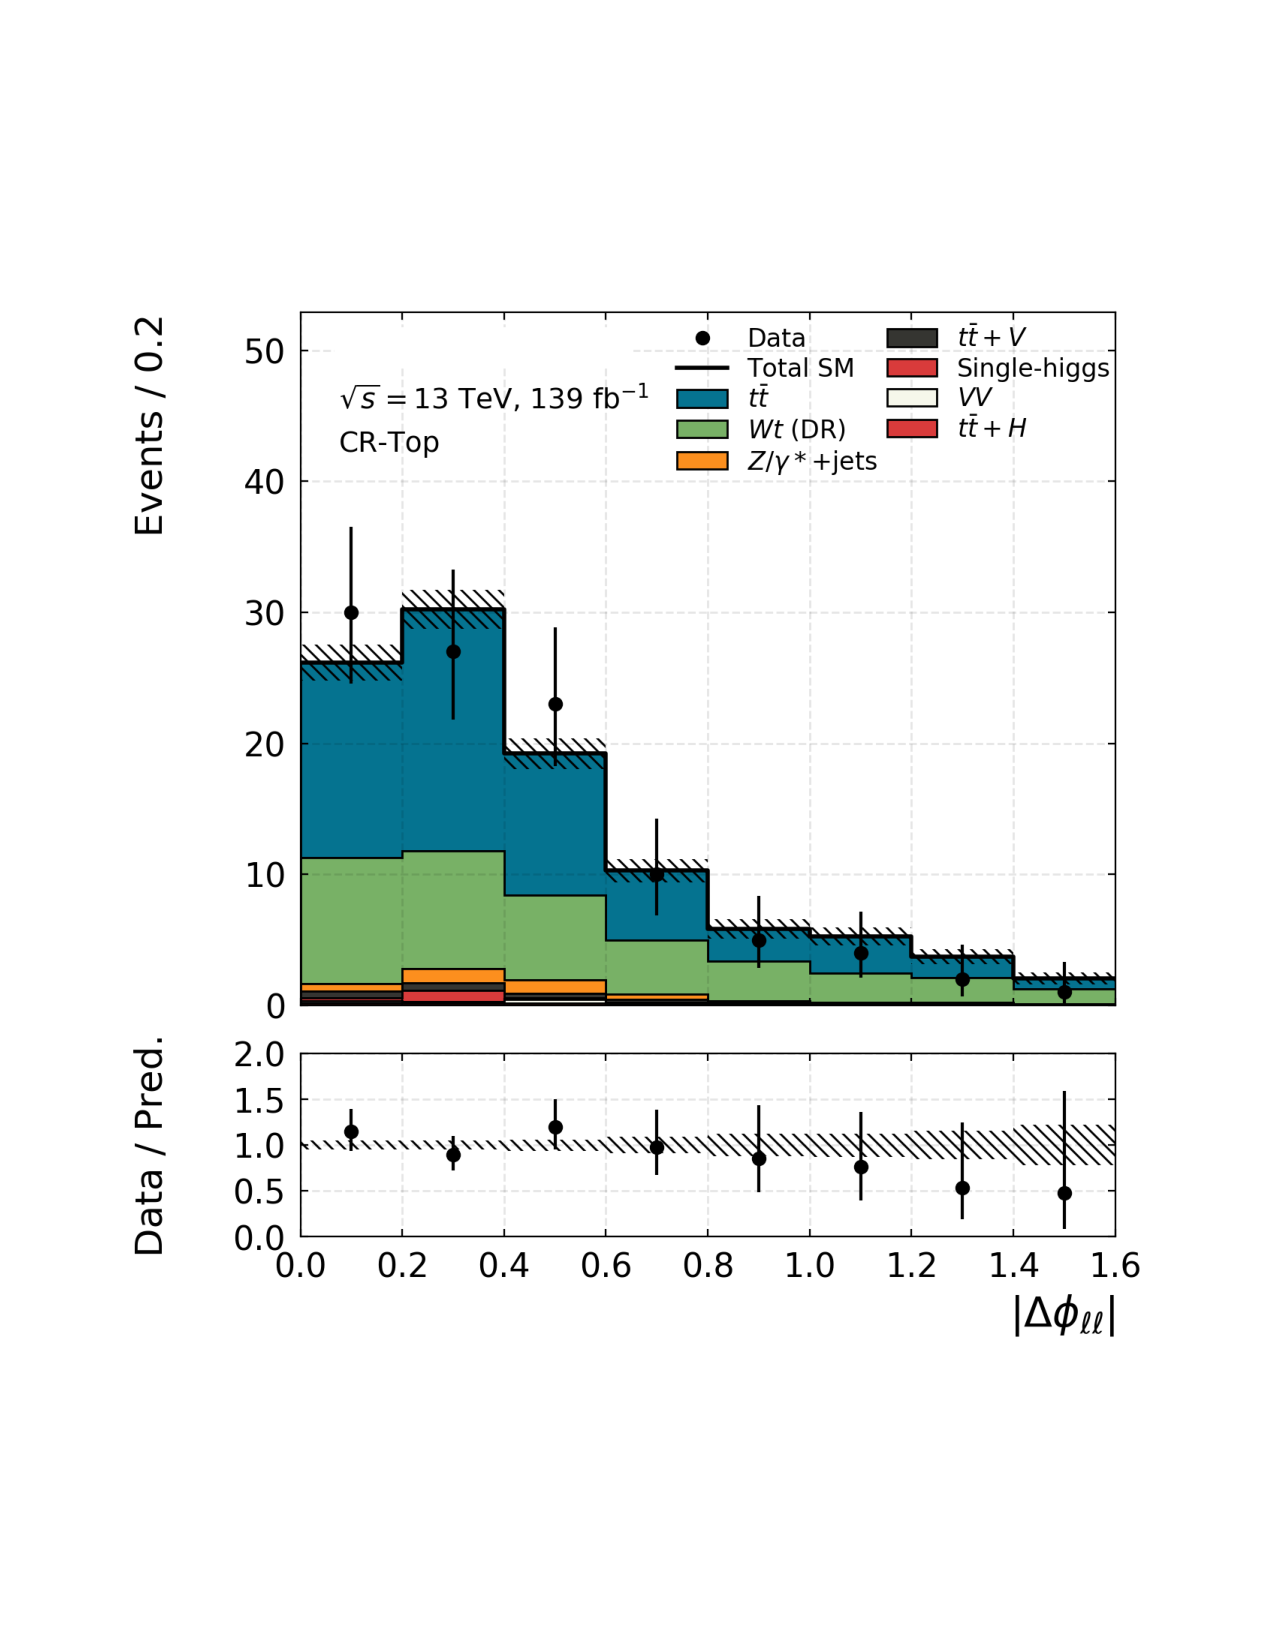
\includegraphics[width=0.4\textwidth]{figures/search_hh/bkg_estimate/crvr/crtop/crtoptest_dphi_ll}
    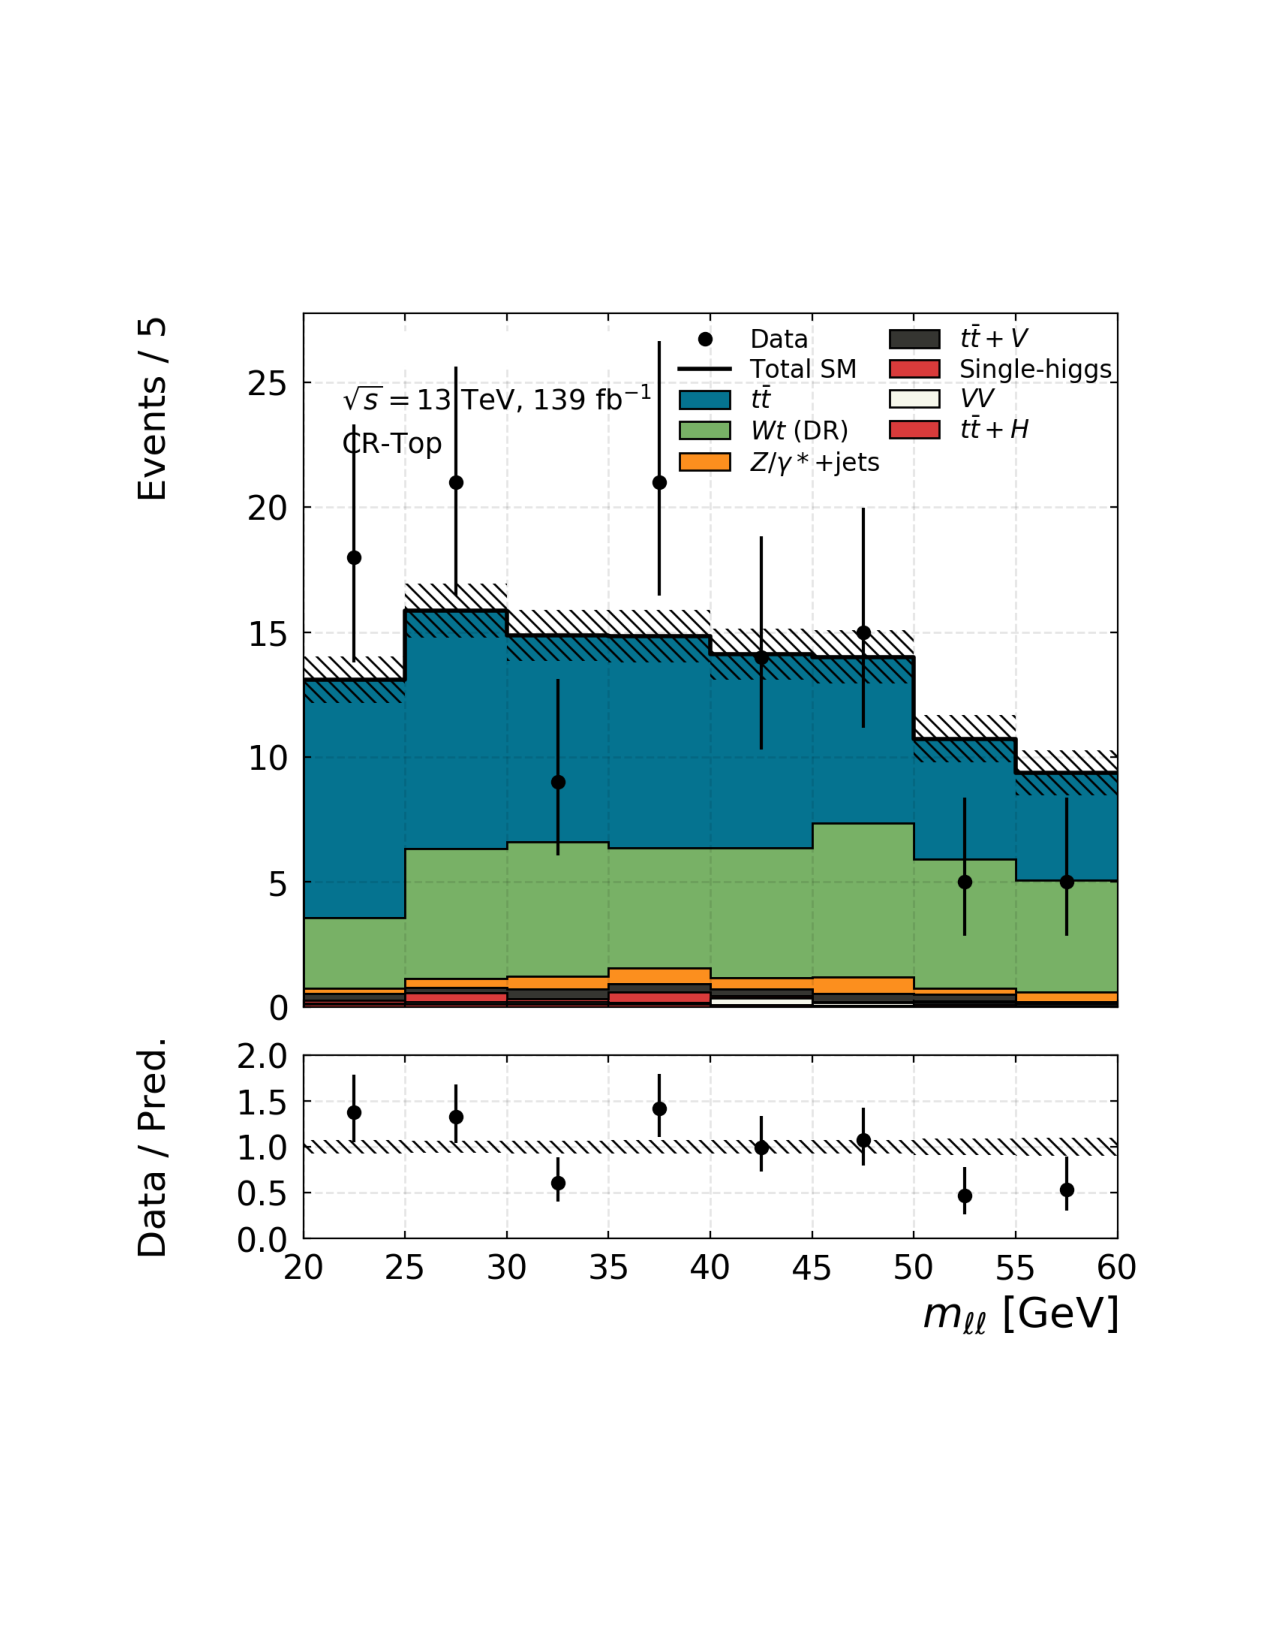
\includegraphics[width=0.4\textwidth]{figures/search_hh/bkg_estimate/crvr/crtop/crtoptest_mll}
    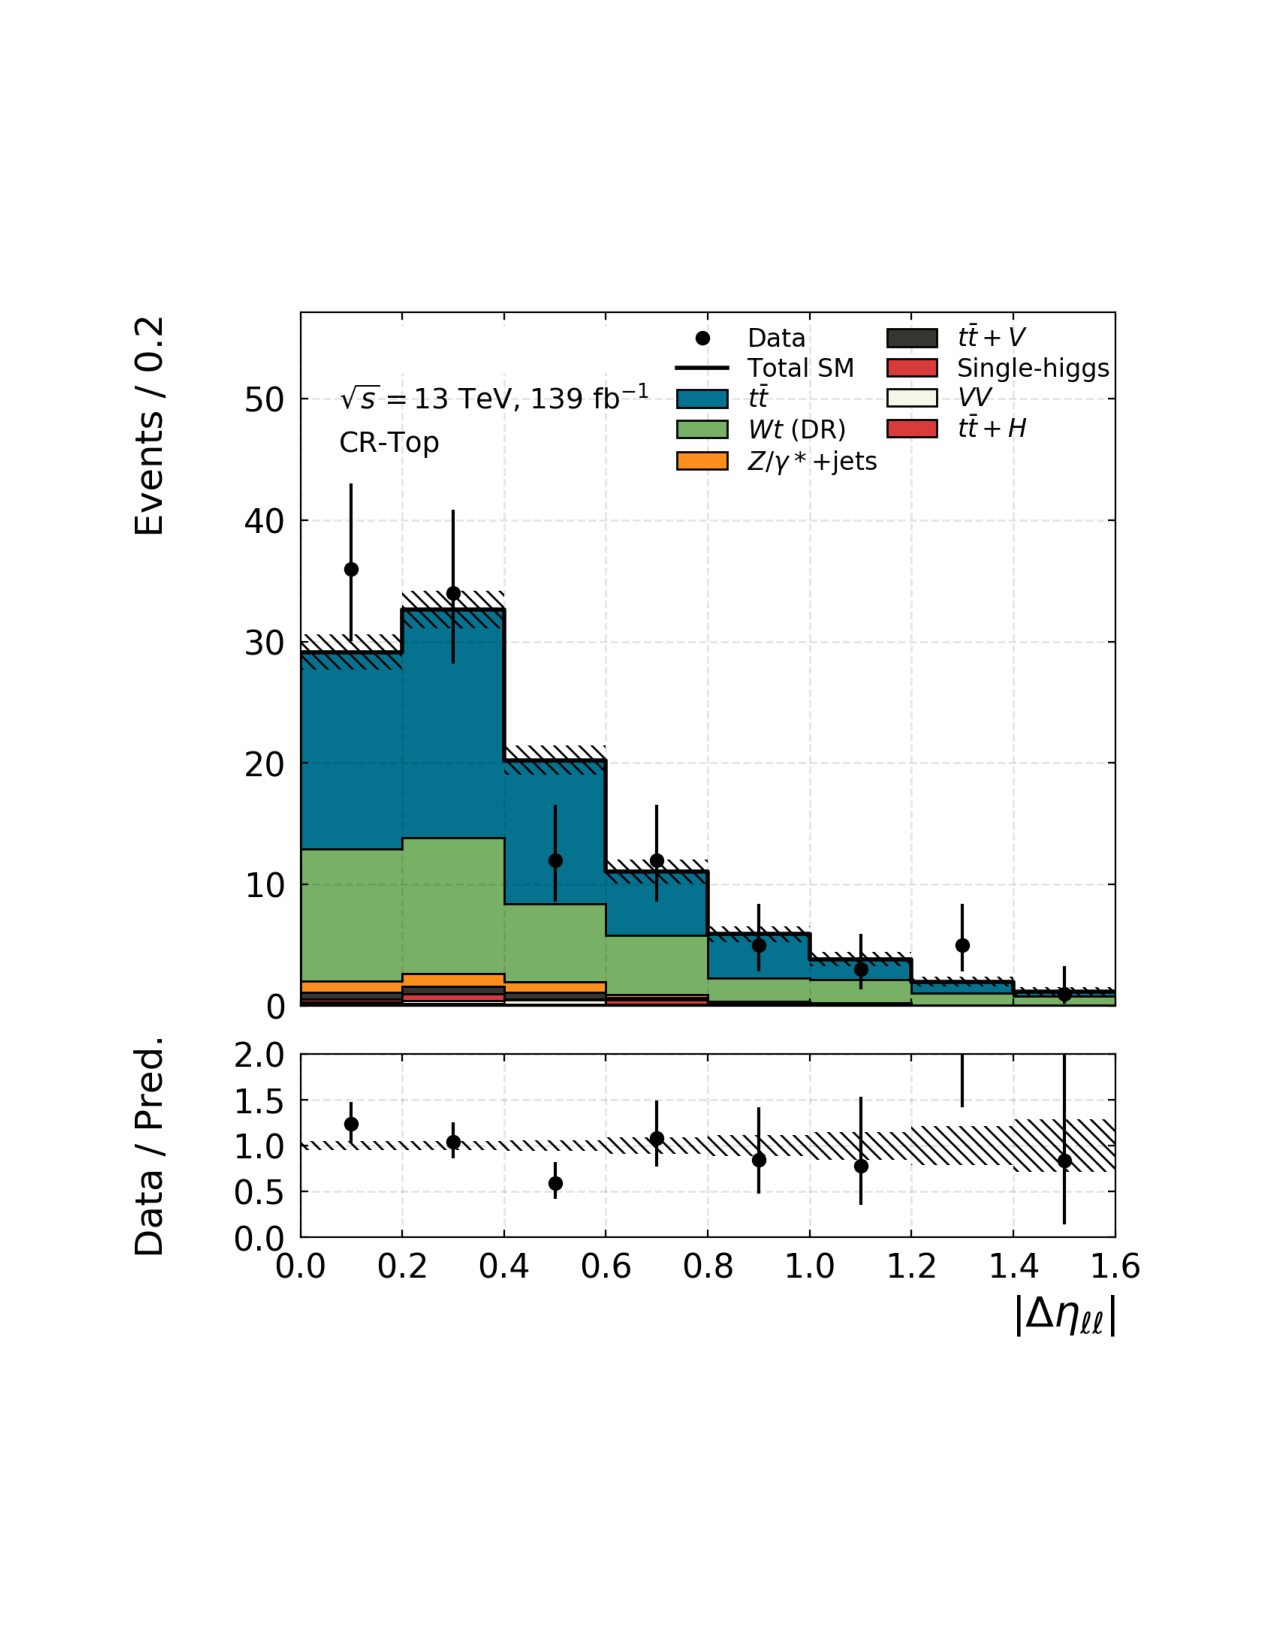
\includegraphics[width=0.4\textwidth]{figures/search_hh/bkg_estimate/crvr/crtop/crtoptest_deta_ll}
    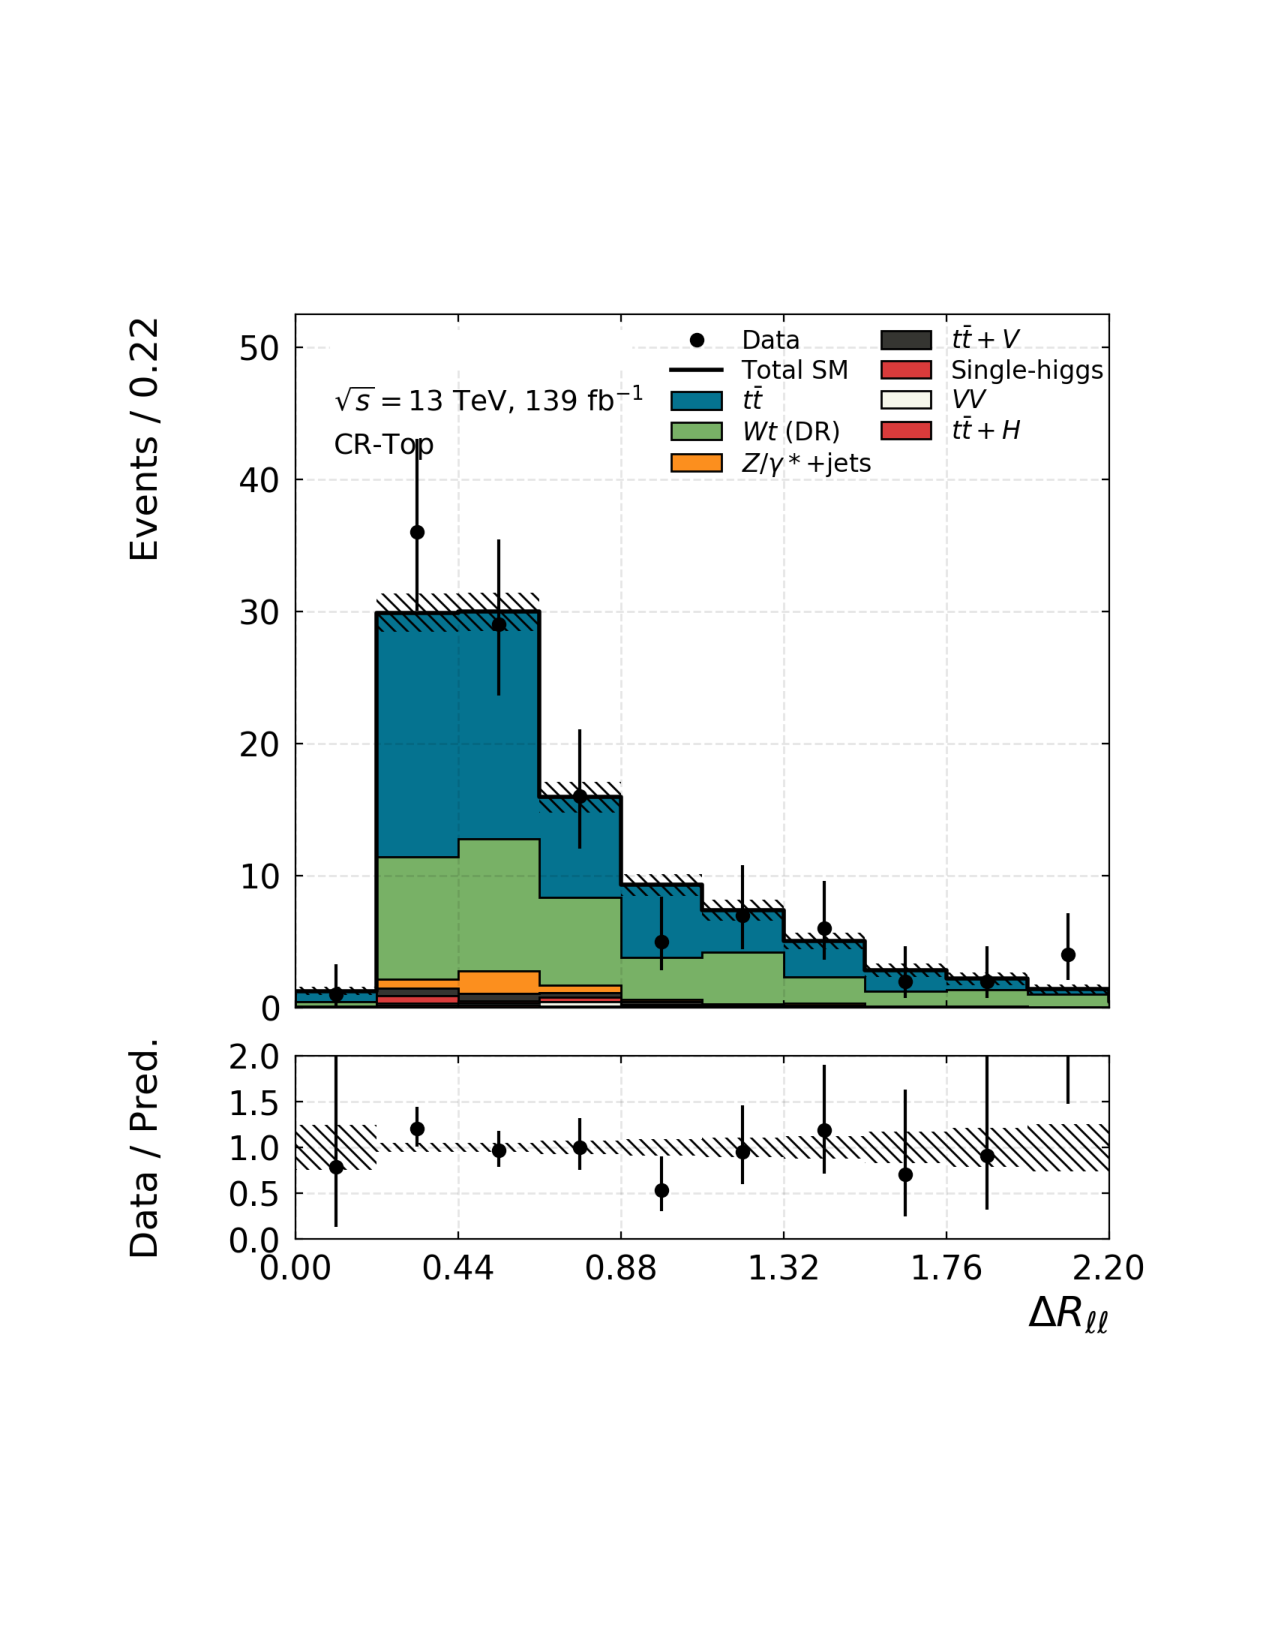
\includegraphics[width=0.4\textwidth]{figures/search_hh/bkg_estimate/crvr/crtop/crtoptest_dRll}
    \caption{
    Kinematic distributions in the Top control region, CR-Top.
    The error bands include only the statistical uncertainty.
    The normalization factors obtained from the background-only fit (Table \ref{tab:hh_norm_factors}) are applied
    to the Top (\ttbar~and $Wt$) and $Z$+jets MC processes.
    }
    \label{fig:crtop_kin_plots_0}
\end{figure}
\begin{figure}[!htb]
    \centering
    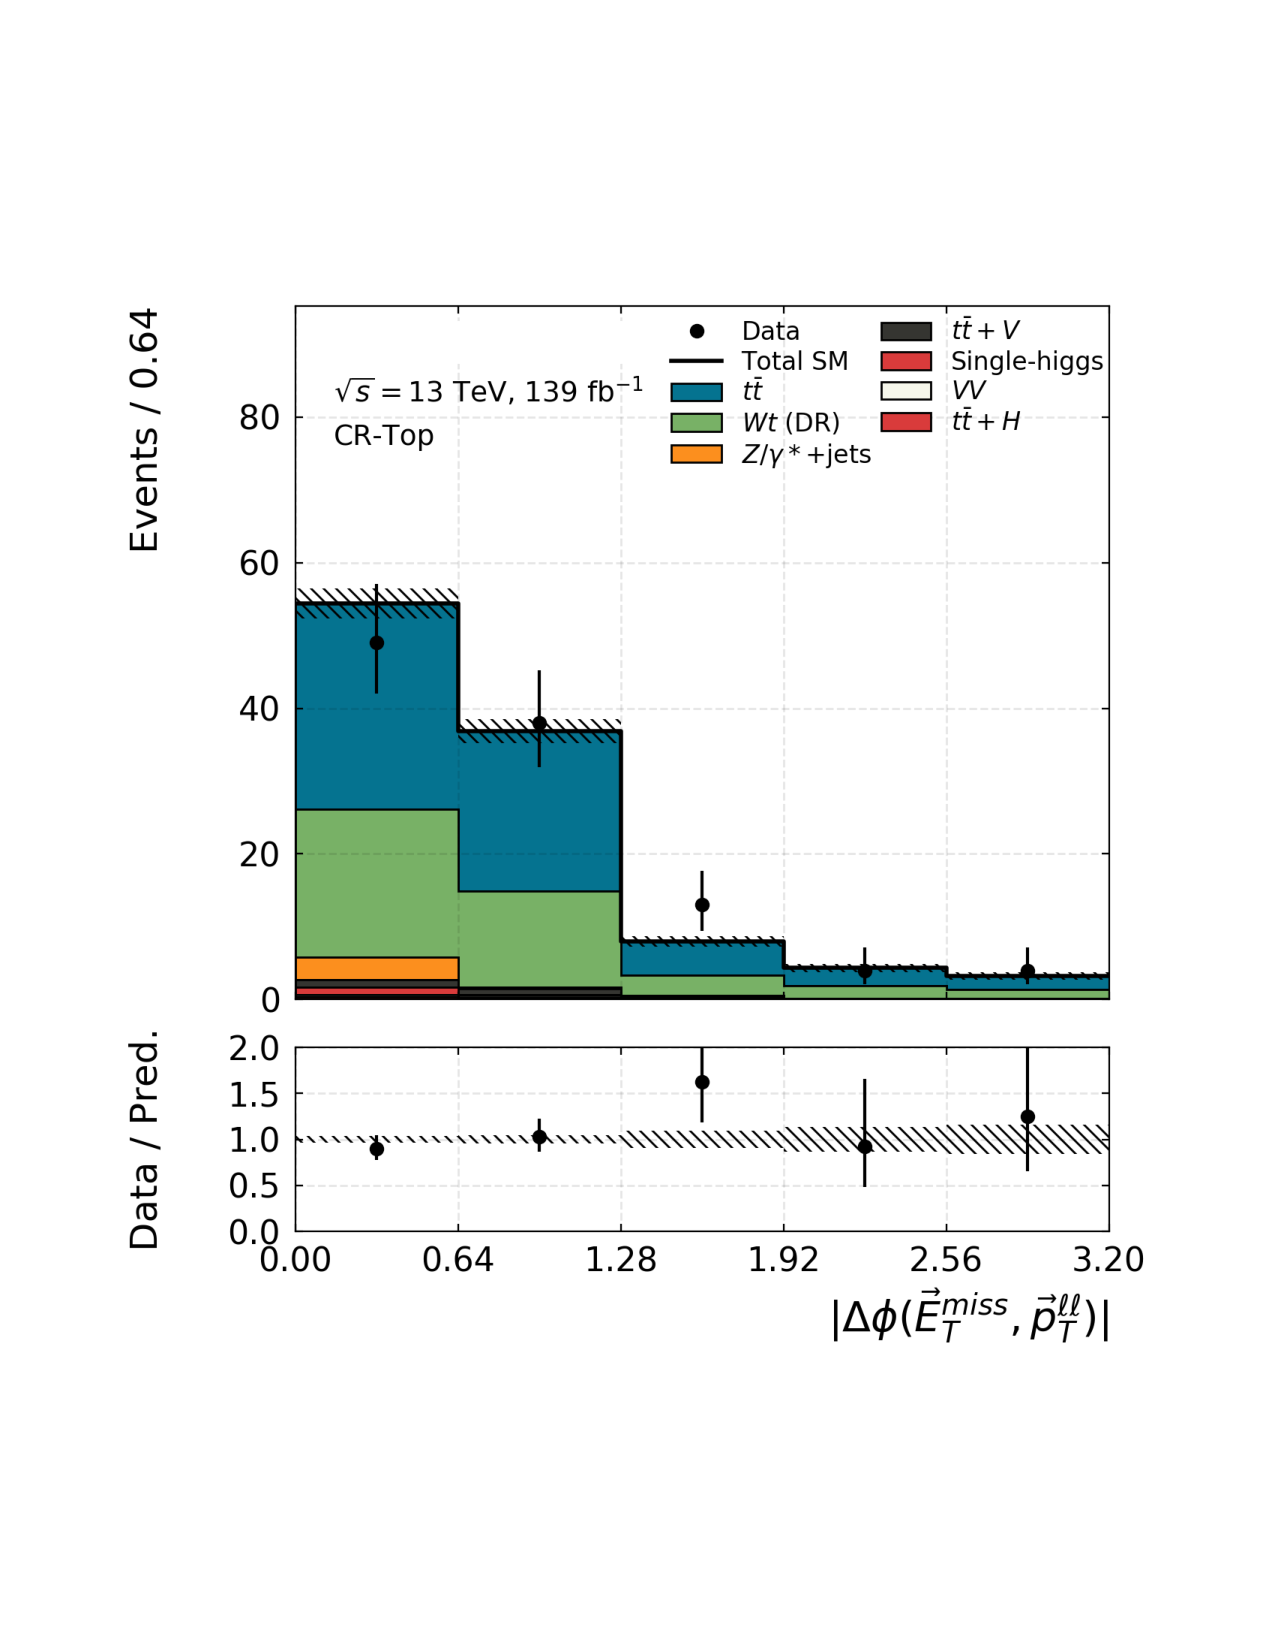
\includegraphics[width=0.4\textwidth]{figures/search_hh/bkg_estimate/crvr/crtop/crtoptest_dphi_met_ll}
    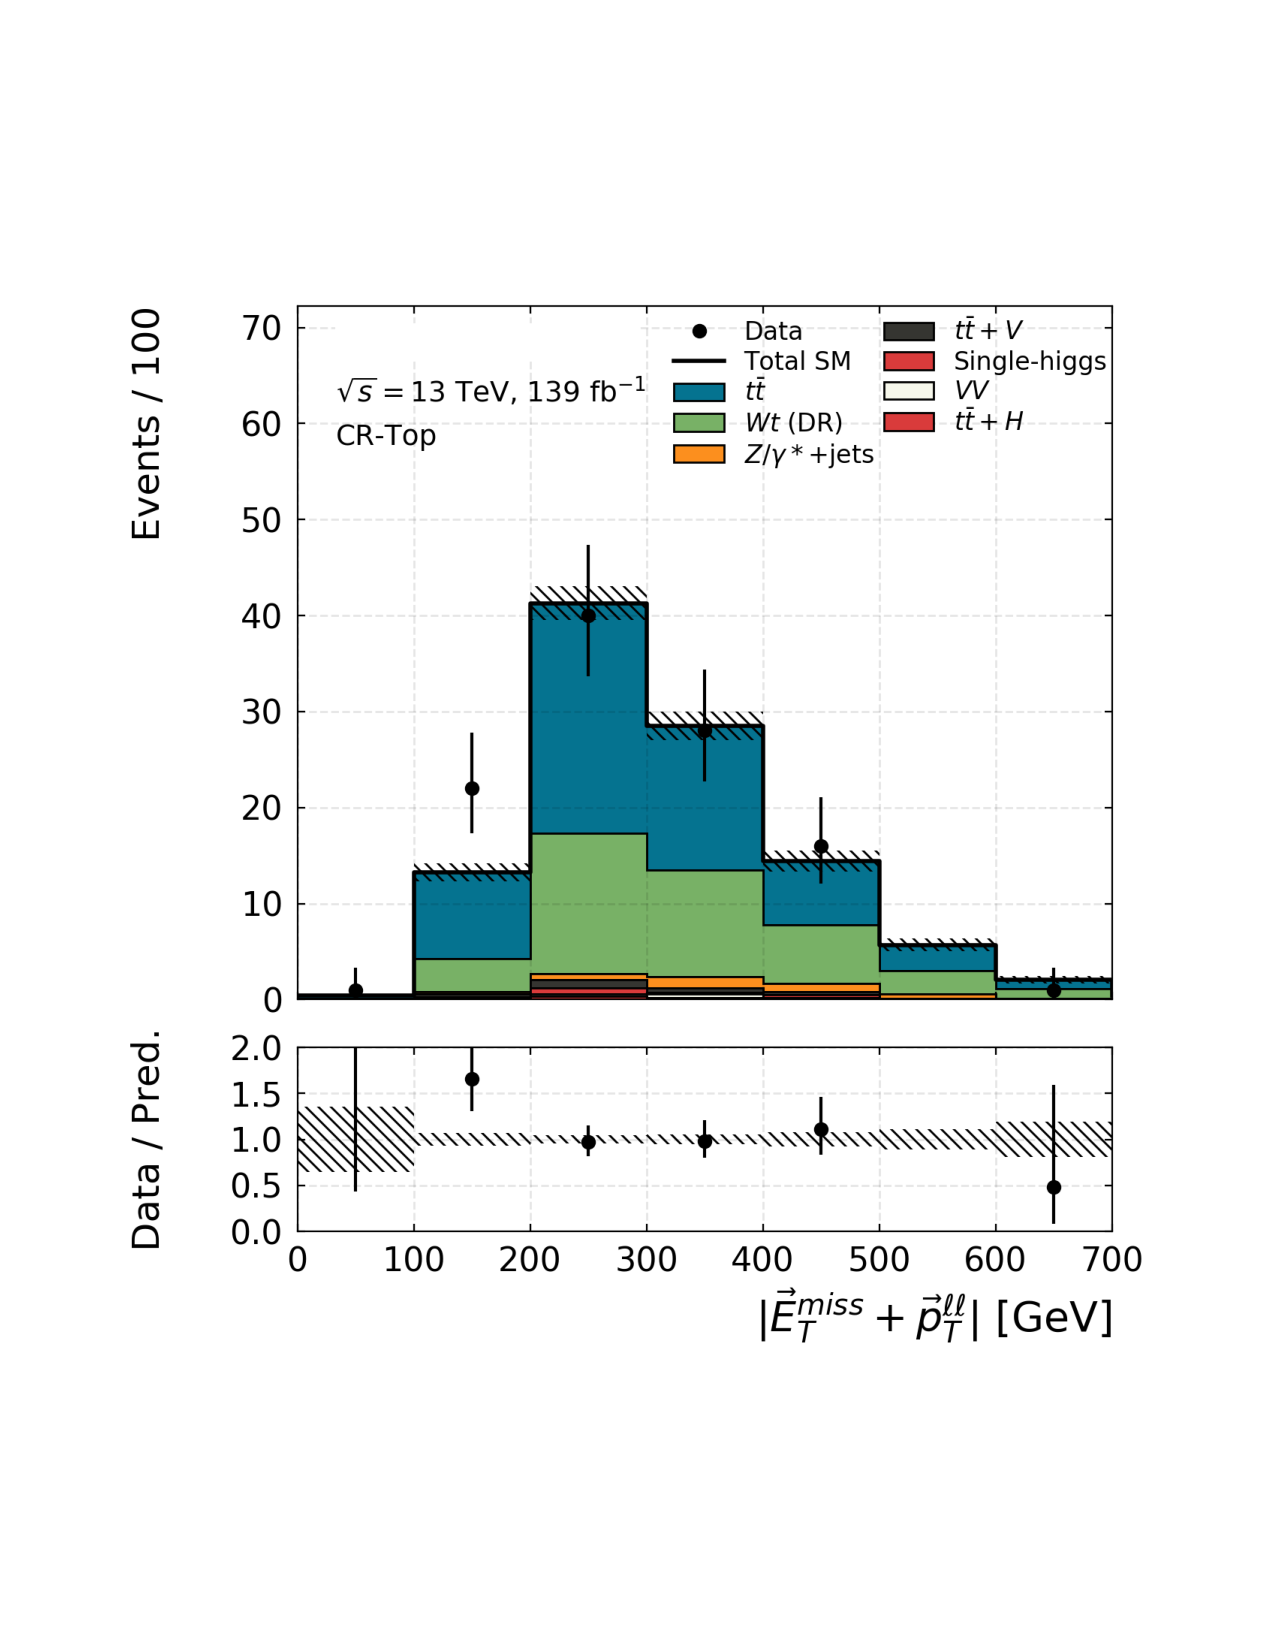
\includegraphics[width=0.4\textwidth]{figures/search_hh/bkg_estimate/crvr/crtop/crtoptest_met_pTll}
    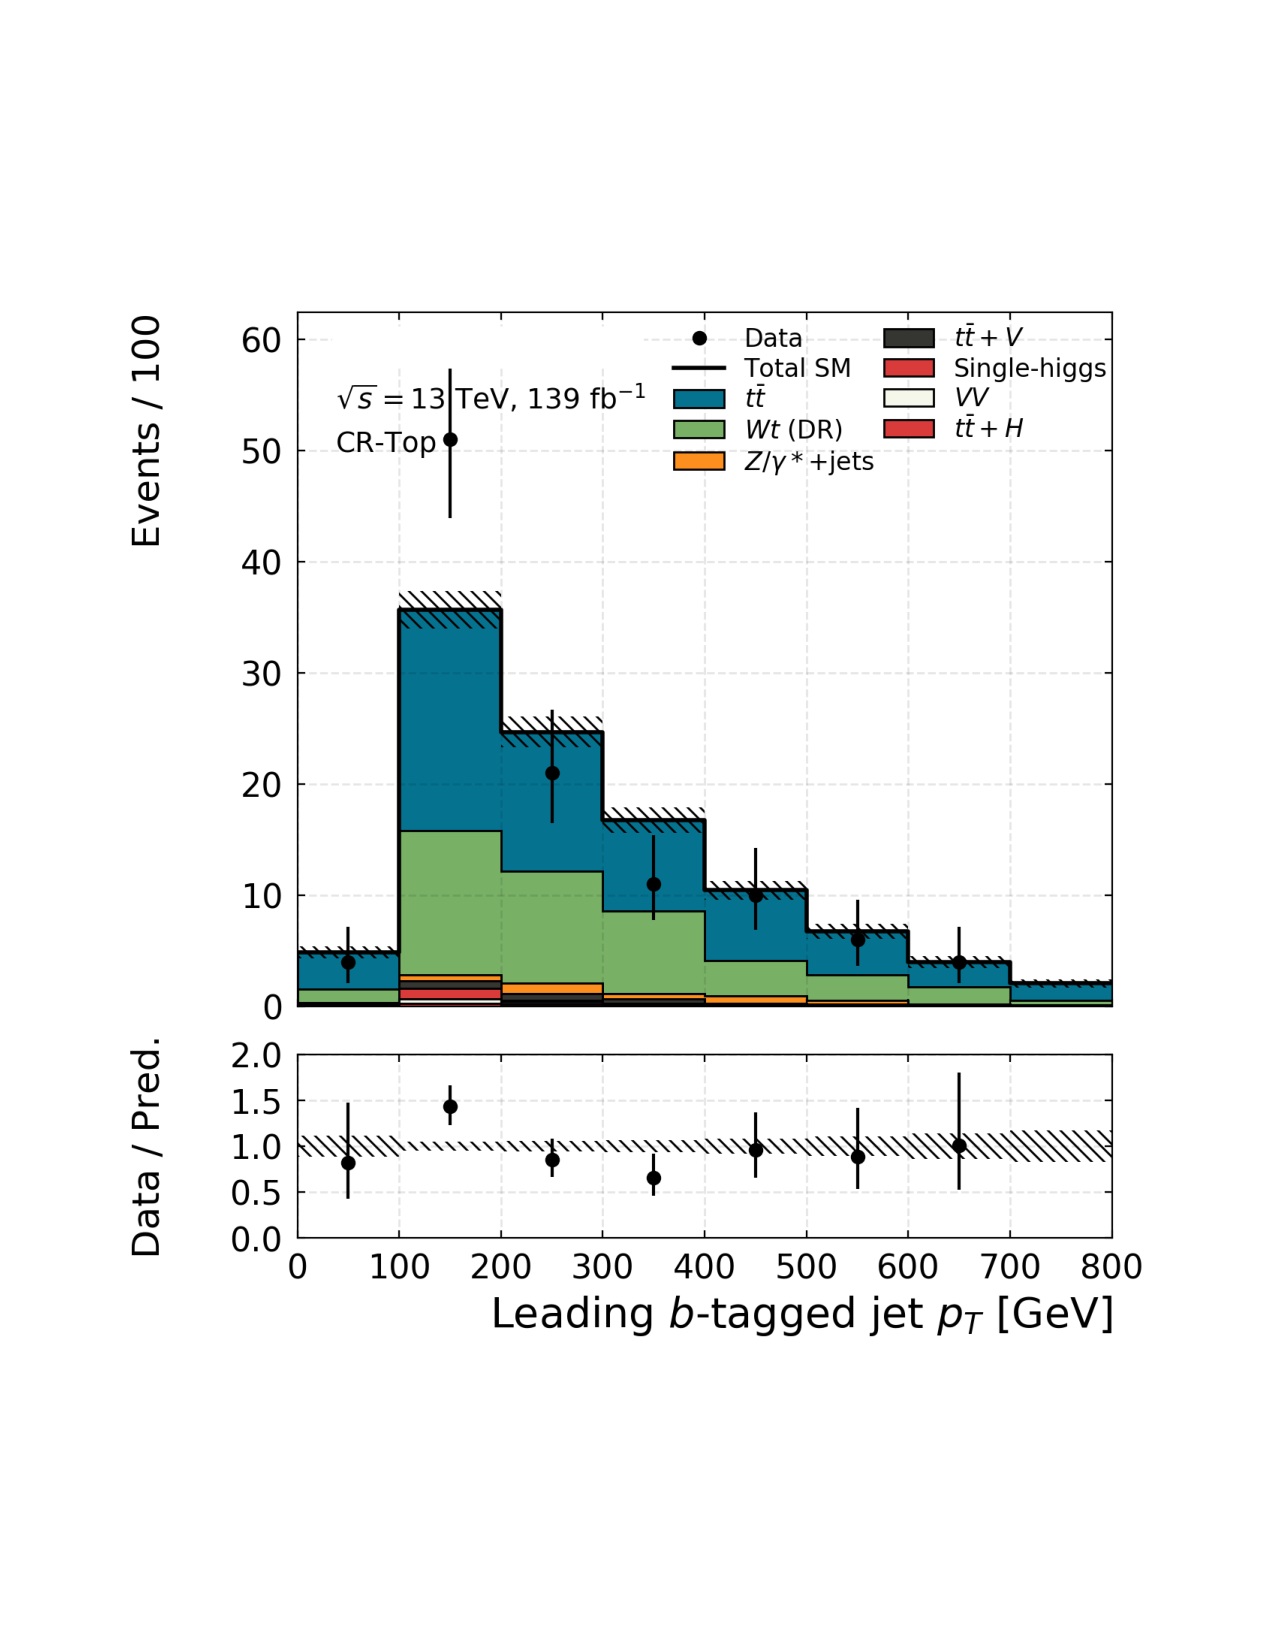
\includegraphics[width=0.4\textwidth]{figures/search_hh/bkg_estimate/crvr/crtop/crtoptest_bj0_pt}
    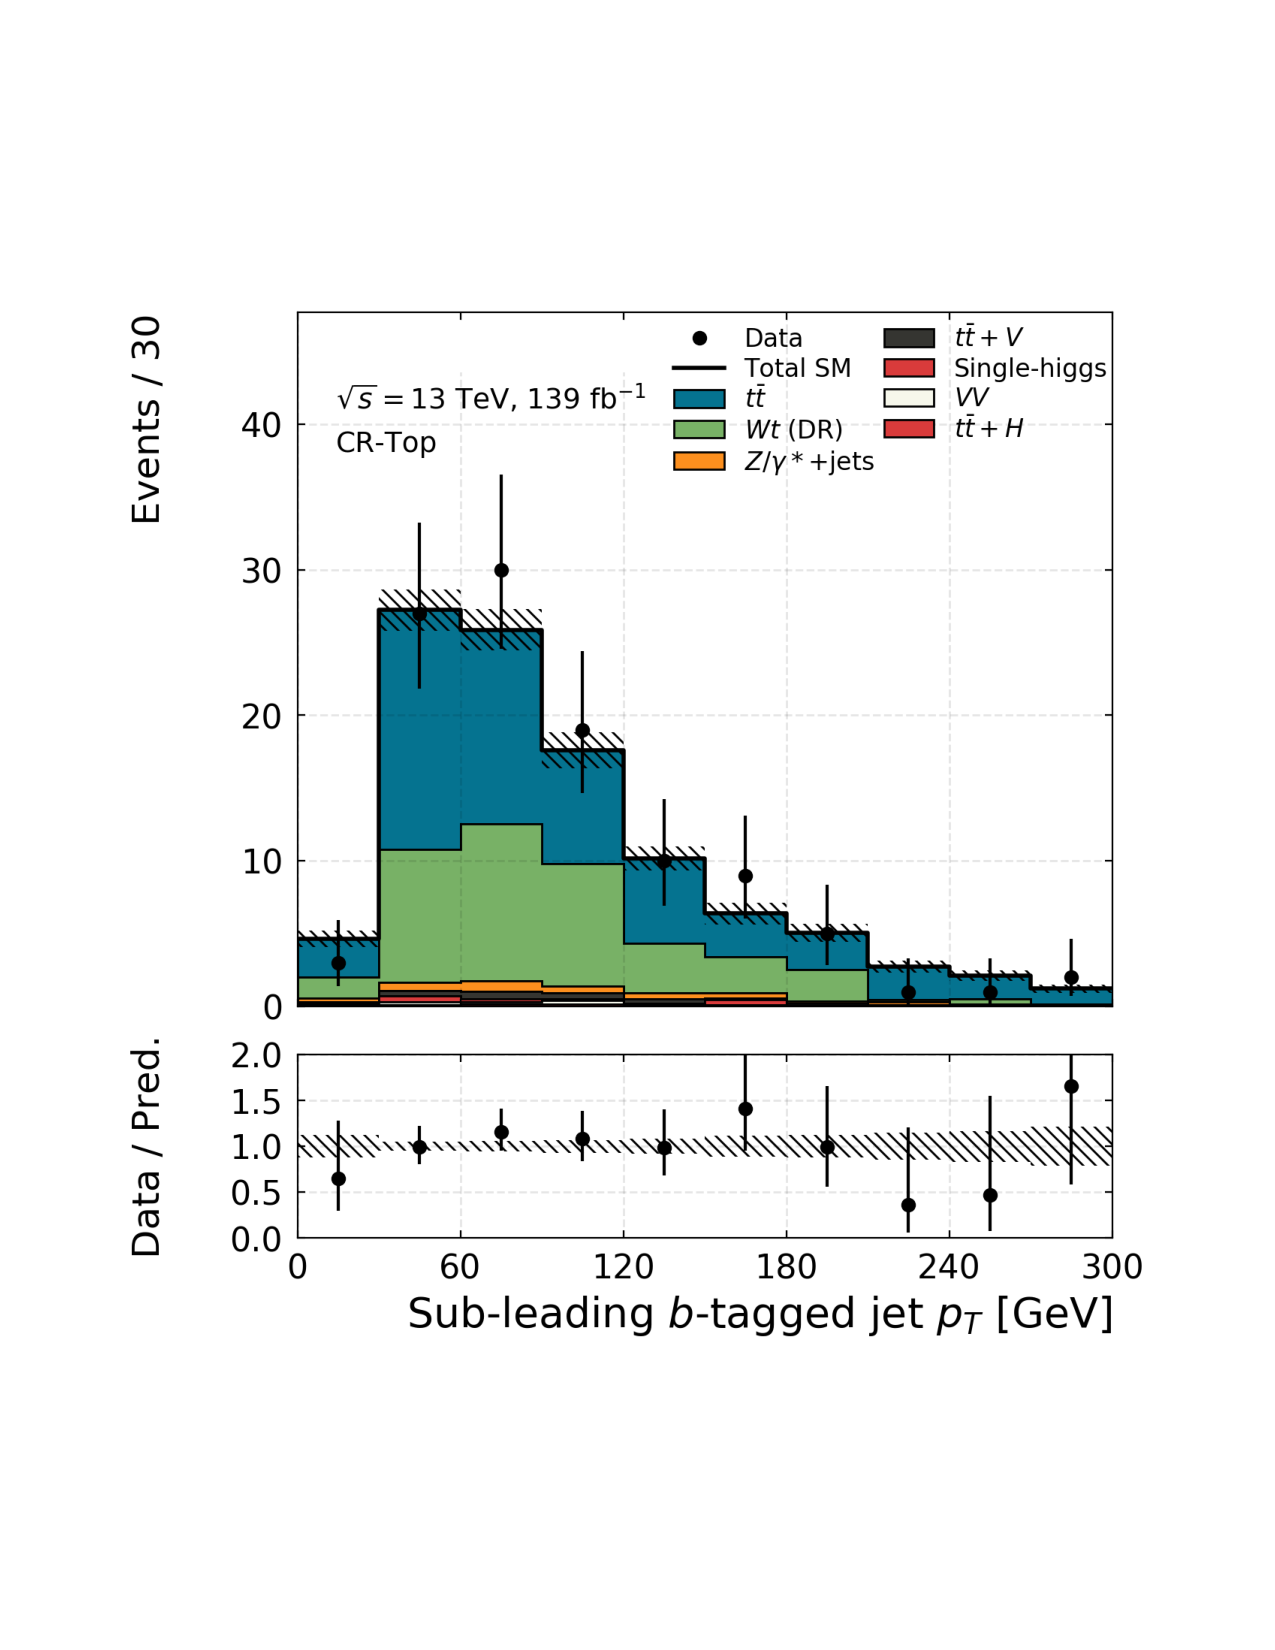
\includegraphics[width=0.4\textwidth]{figures/search_hh/bkg_estimate/crvr/crtop/crtoptest_bj1_pt}
    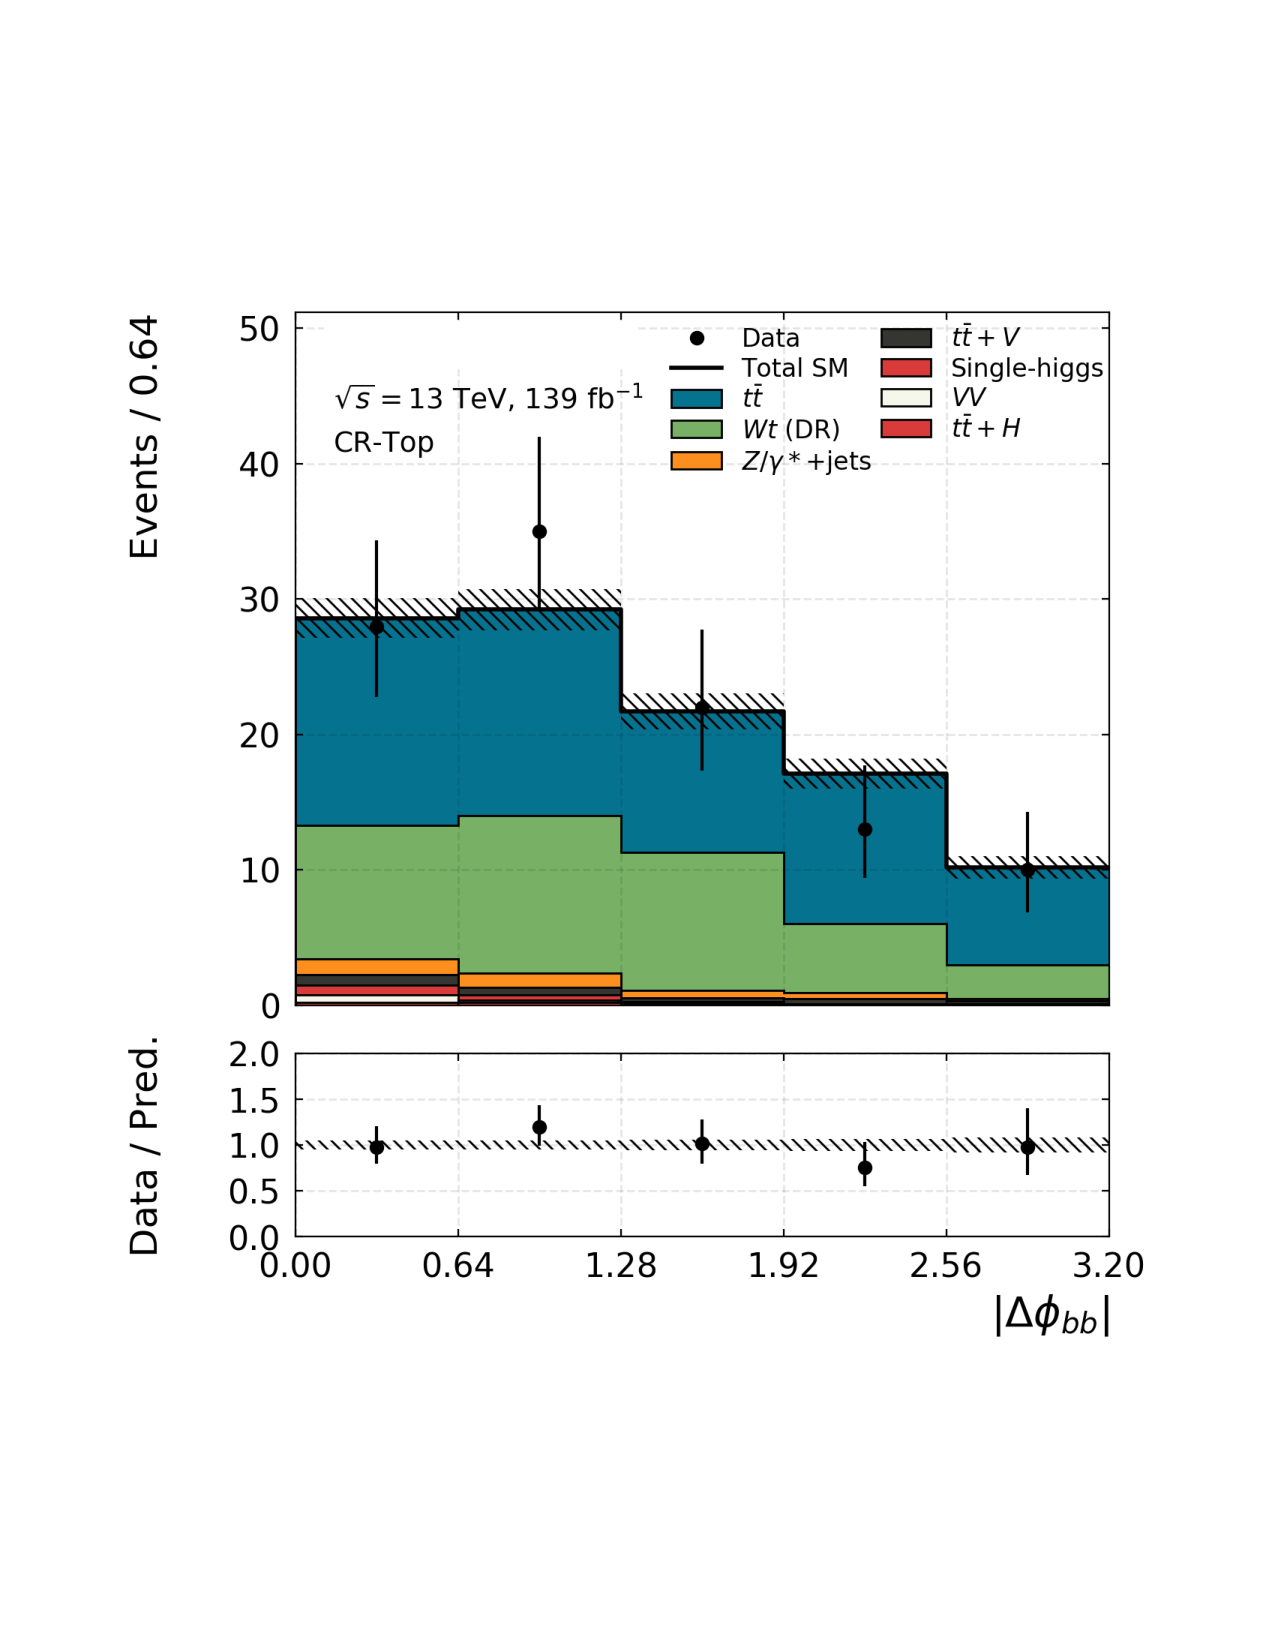
\includegraphics[width=0.4\textwidth]{figures/search_hh/bkg_estimate/crvr/crtop/crtoptest_dphi_bb}
    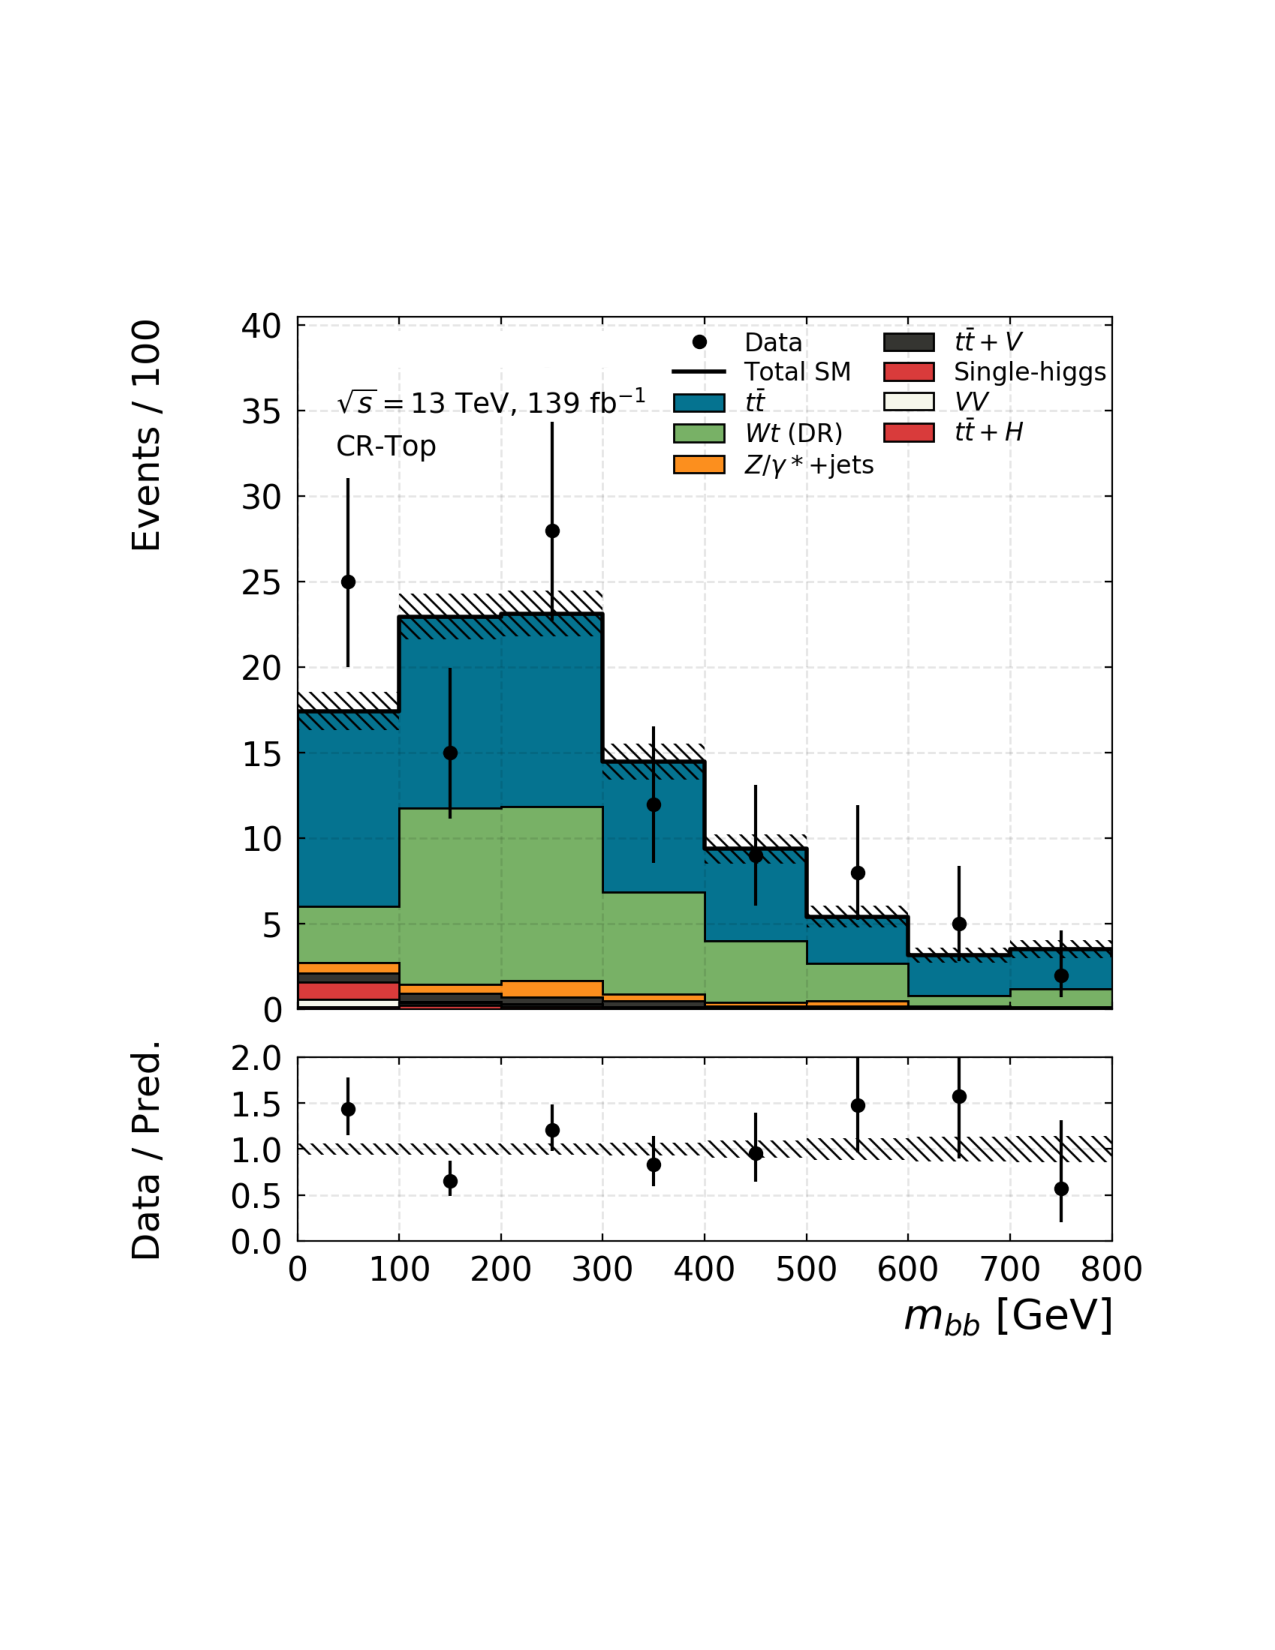
\includegraphics[width=0.4\textwidth]{figures/search_hh/bkg_estimate/crvr/crtop/crtoptest_mbb}
    \caption{
    Kinematic distributions in the Top control region, CR-Top.
    The error bands include only the statistical uncertainty.
    The normalization factors obtained from the background-only fit (Table \ref{tab:hh_norm_factors}) are applied
    to the Top (\ttbar~and $Wt$) and $Z$+jets MC processes.
    }
    \label{fig:crtop_kin_plots_1}
\end{figure}
\begin{figure}[!htb]
    \centering
    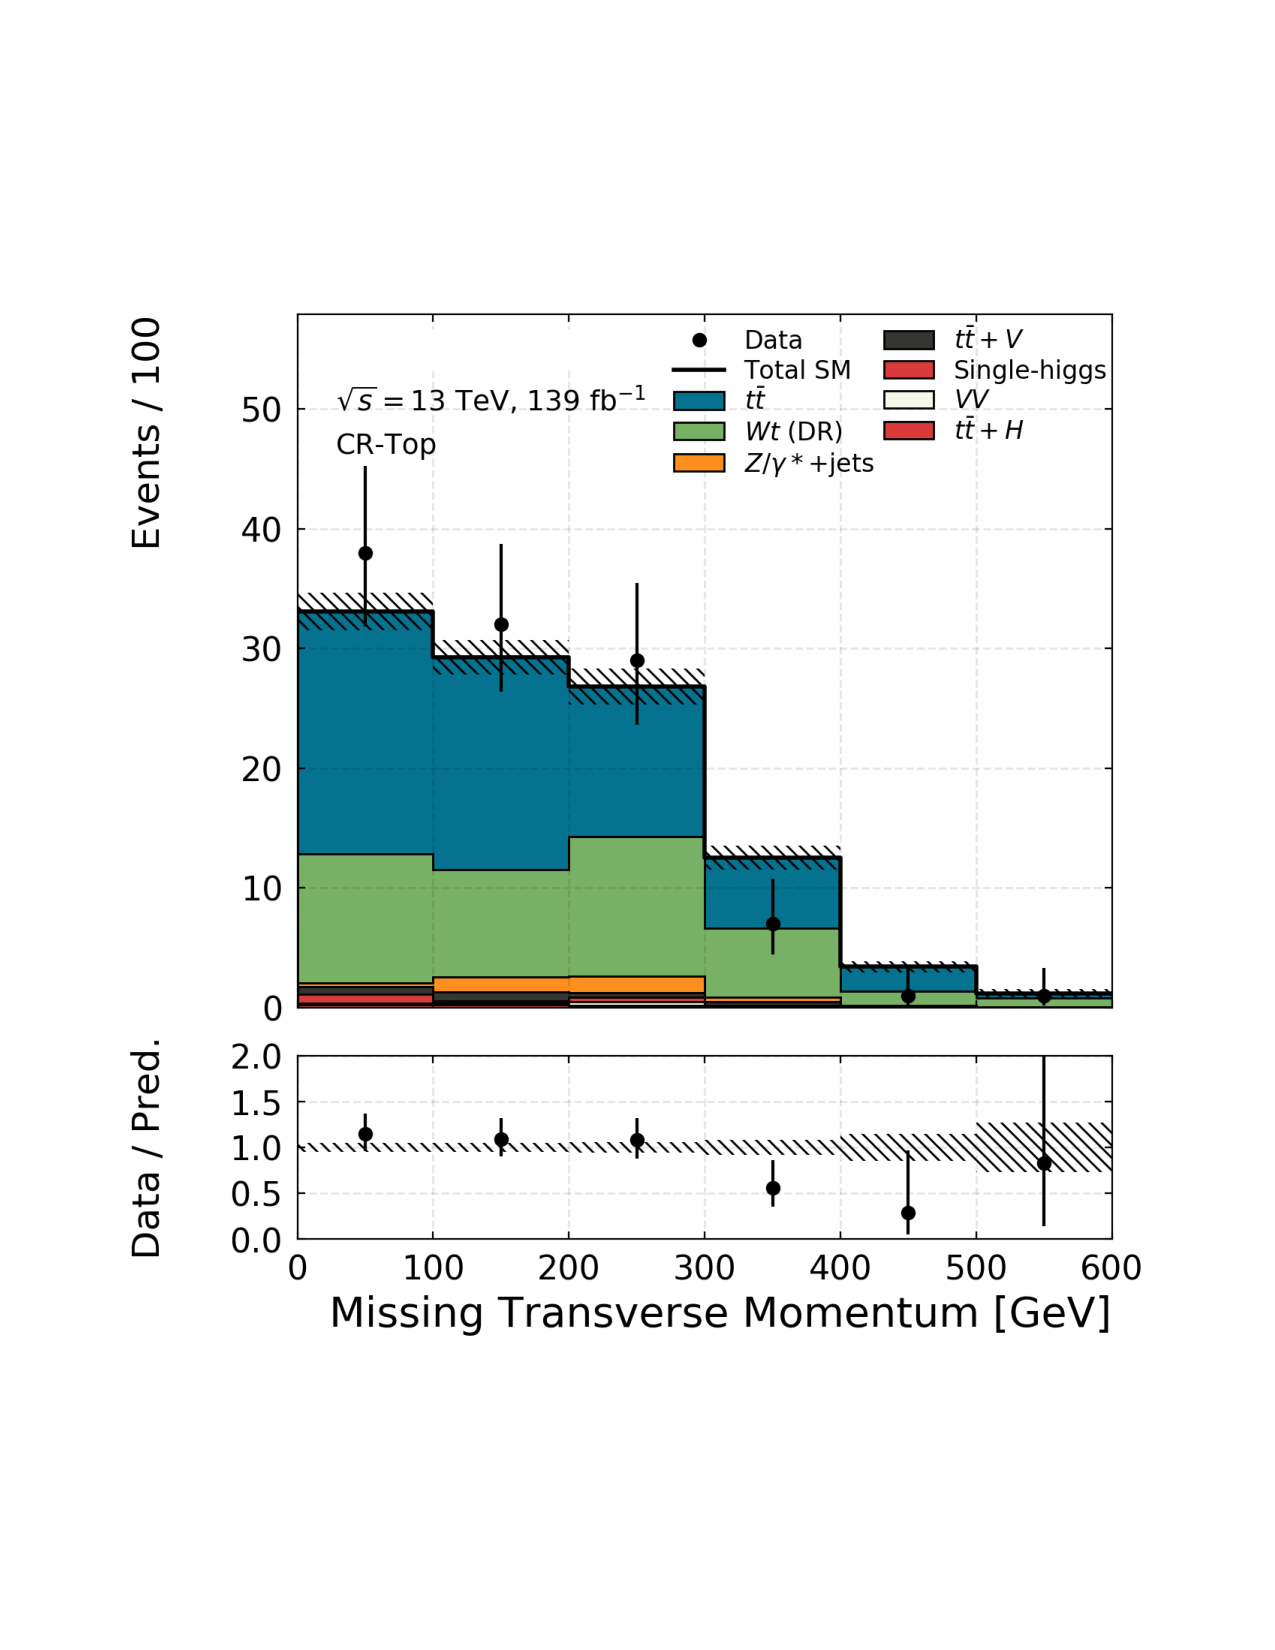
\includegraphics[width=0.4\textwidth]{figures/search_hh/bkg_estimate/crvr/crtop/crtoptest_met}
    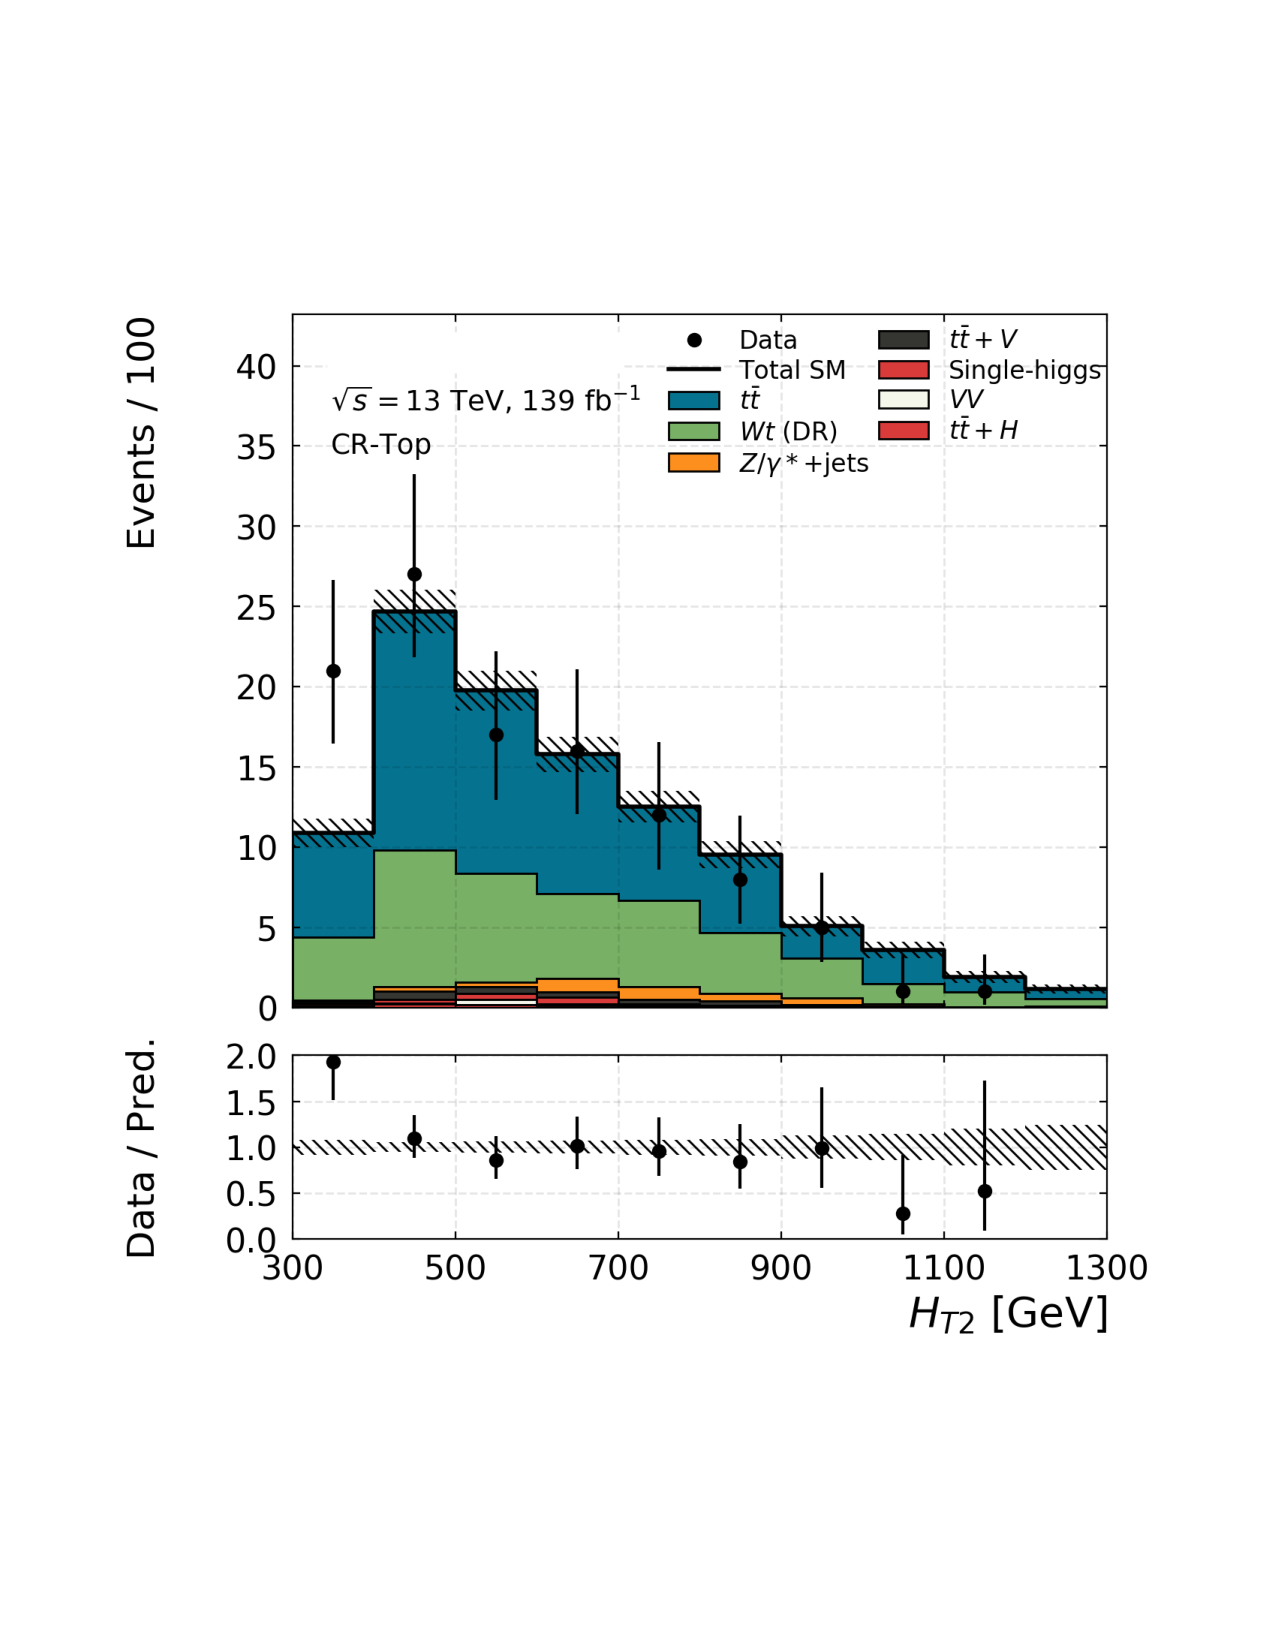
\includegraphics[width=0.4\textwidth]{figures/search_hh/bkg_estimate/crvr/crtop/crtoptest_HT2}
    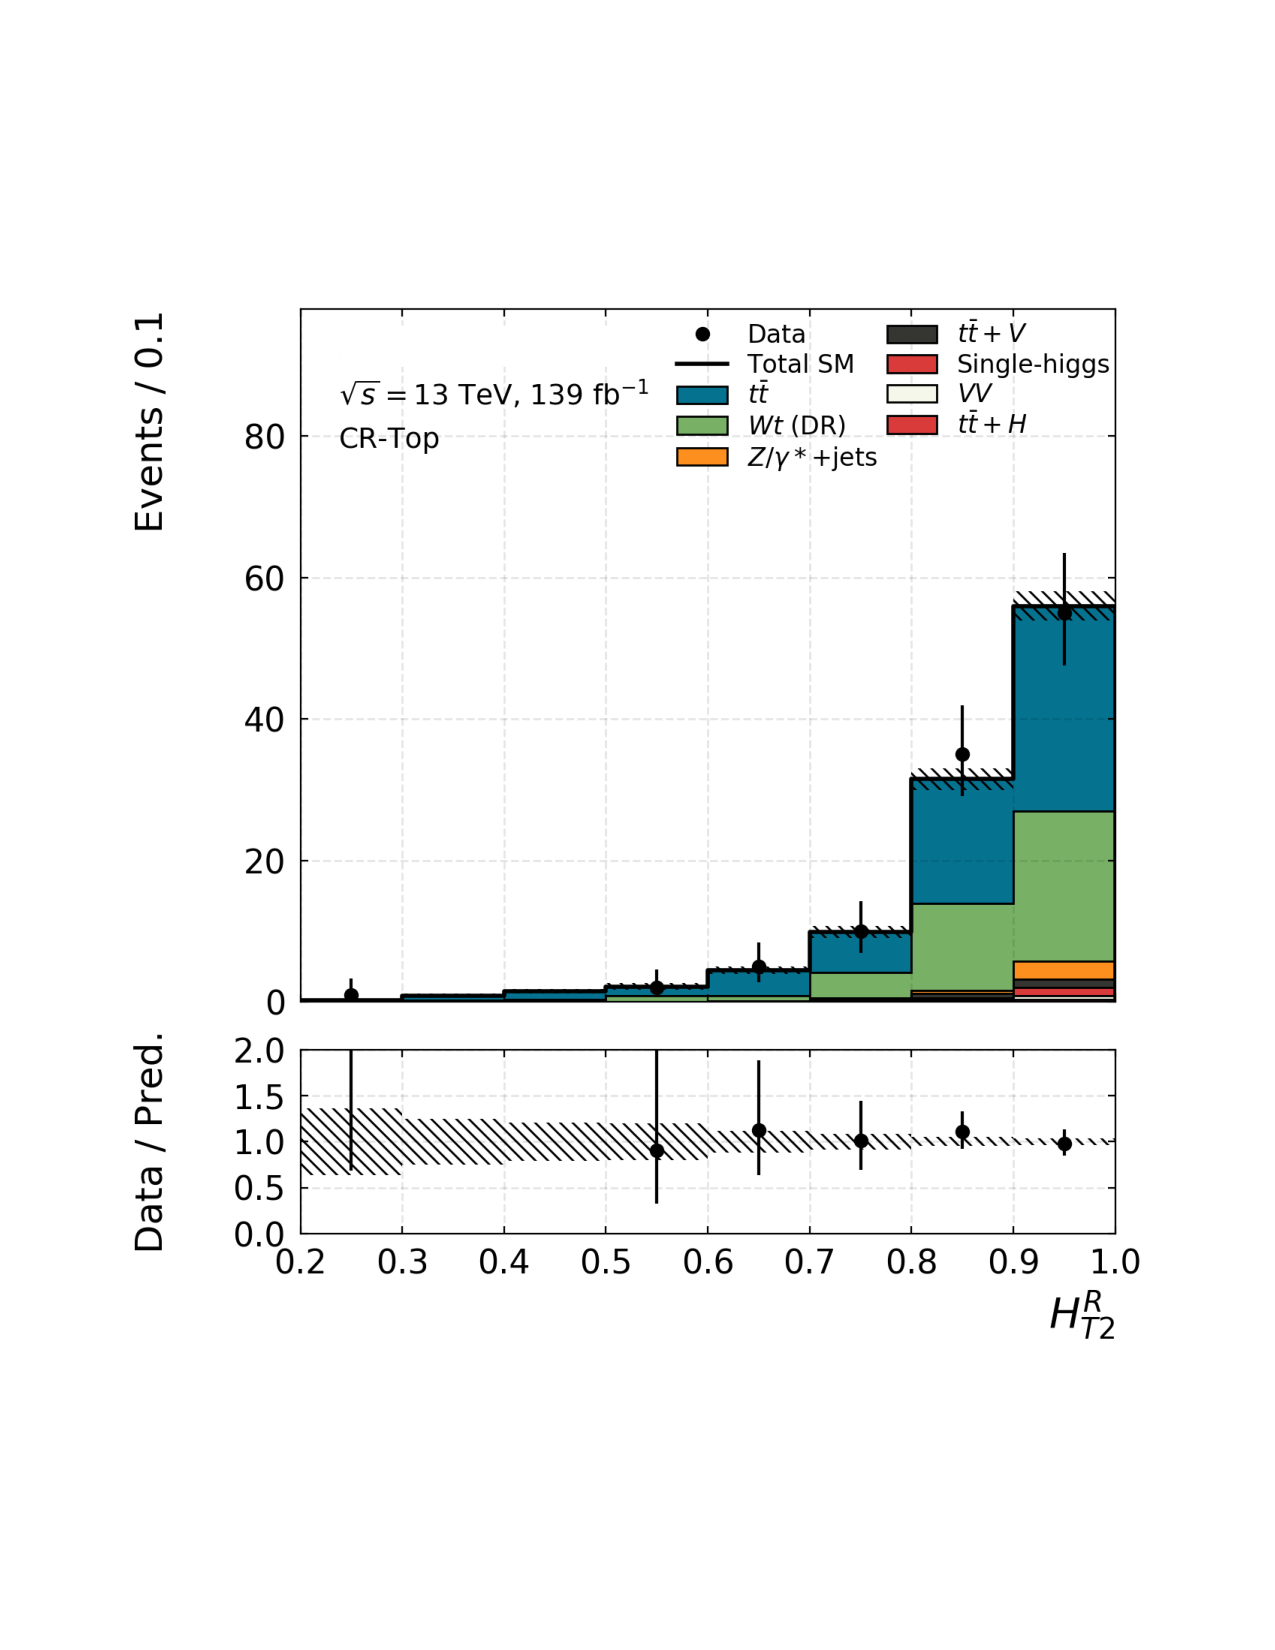
\includegraphics[width=0.4\textwidth]{figures/search_hh/bkg_estimate/crvr/crtop/crtoptest_HT2Ratio}
    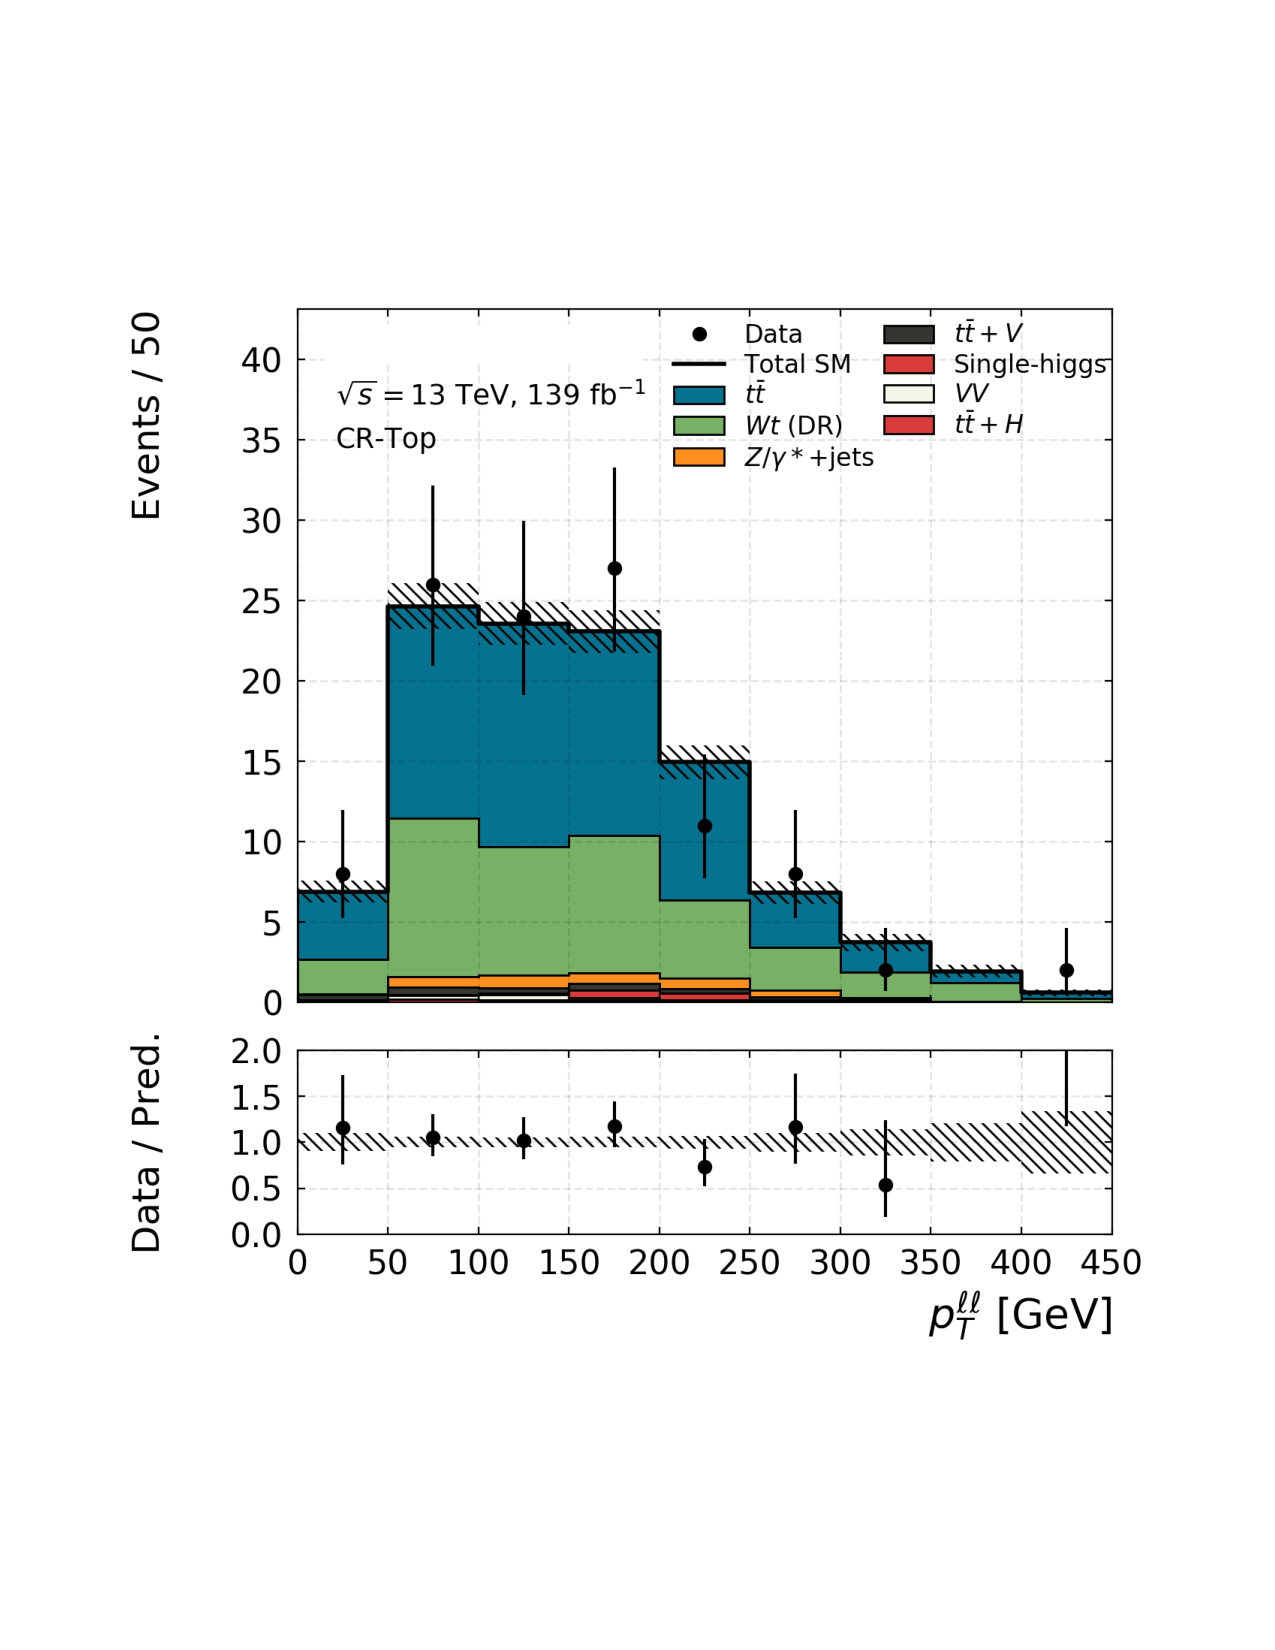
\includegraphics[width=0.4\textwidth]{figures/search_hh/bkg_estimate/crvr/crtop/crtoptest_pTll}
    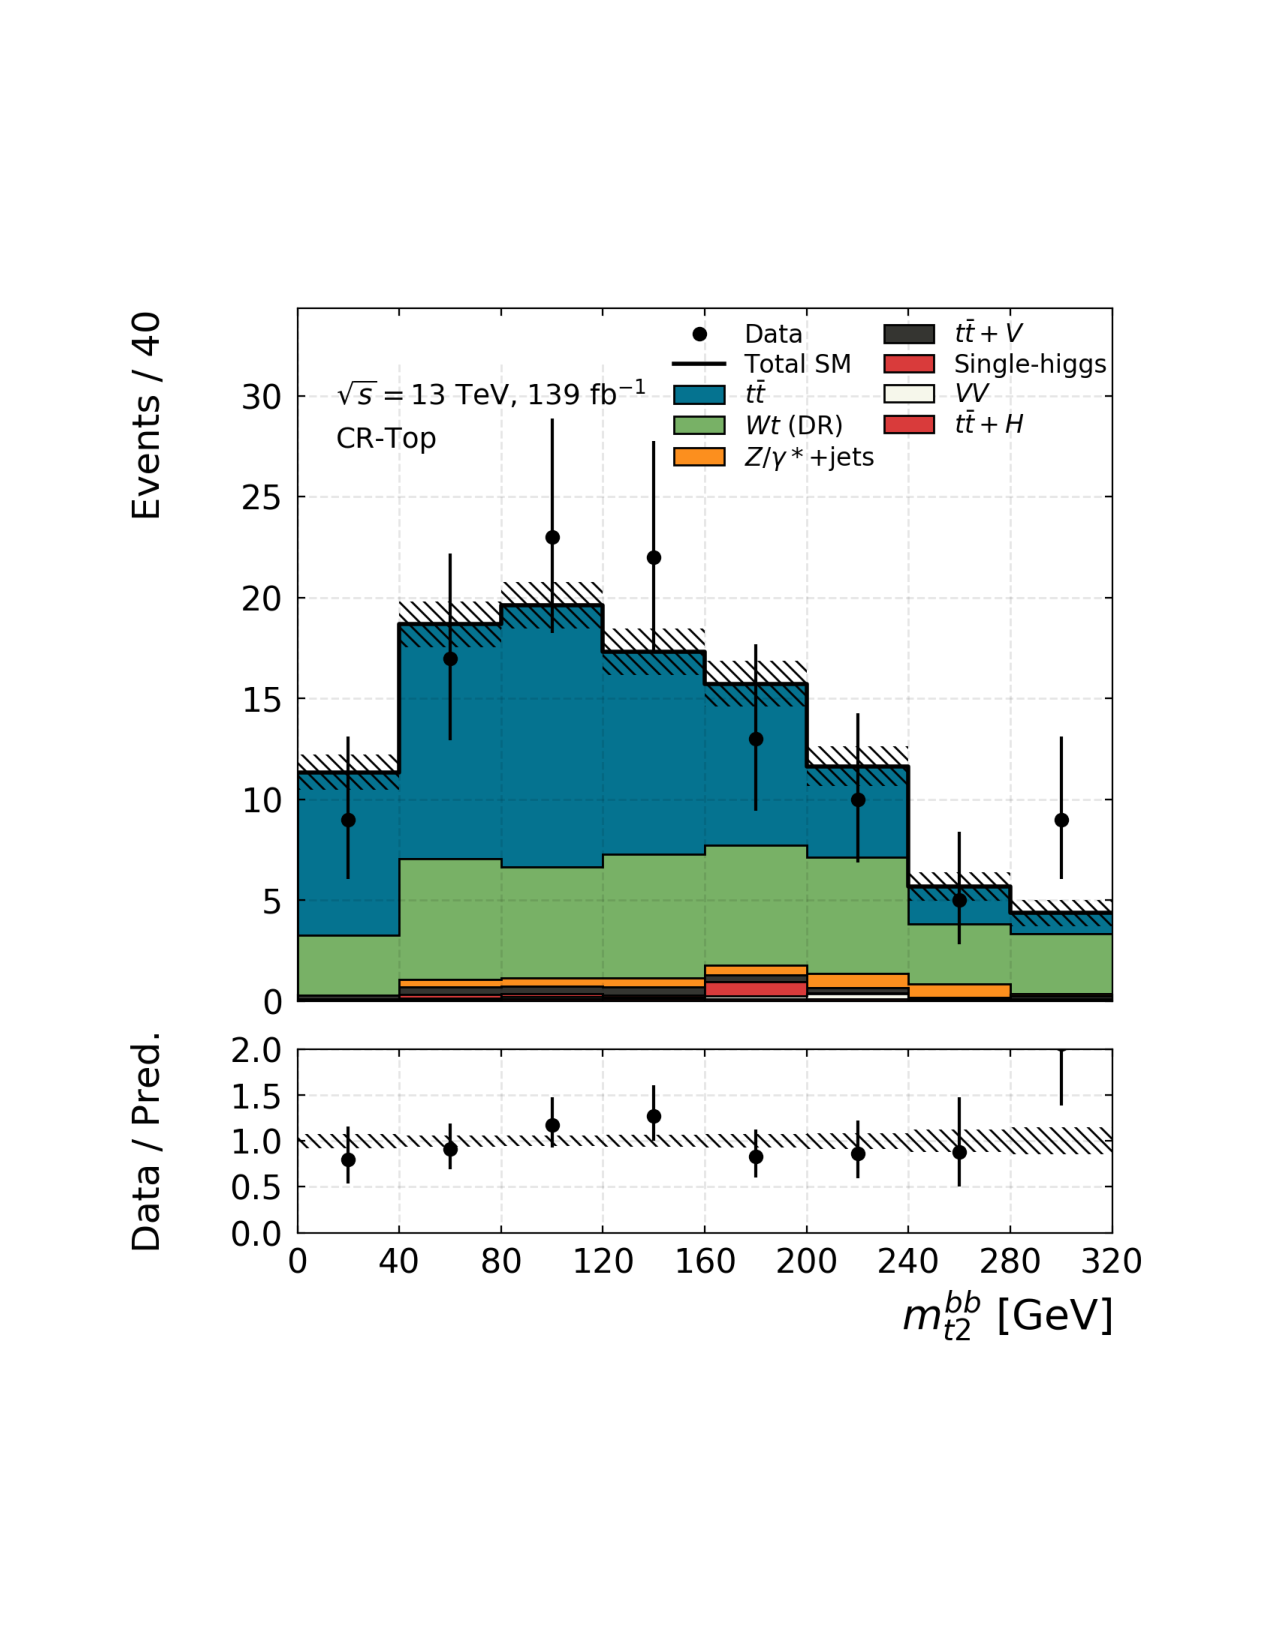
\includegraphics[width=0.4\textwidth]{figures/search_hh/bkg_estimate/crvr/crtop/crtoptest_mt2_bb}
    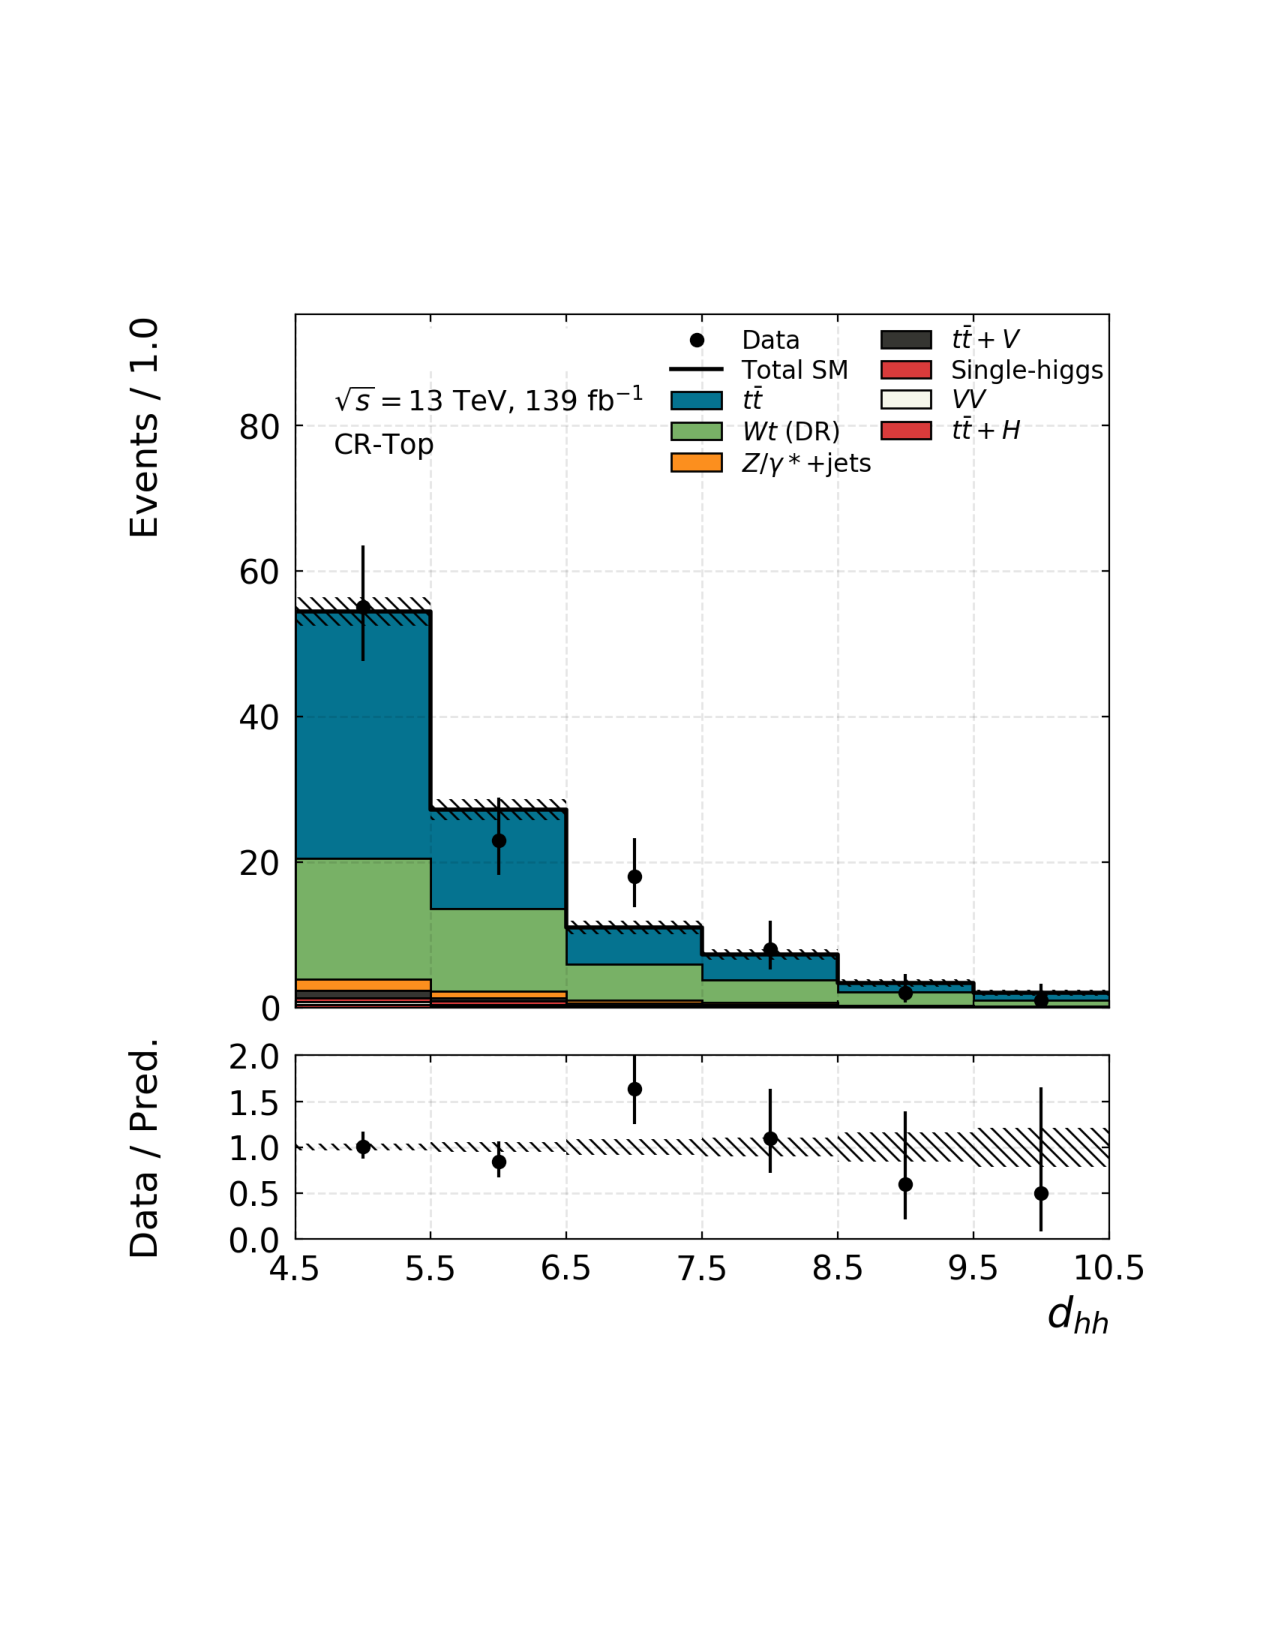
\includegraphics[width=0.4\textwidth]{figures/search_hh/bkg_estimate/crvr/crtop/crtoptest_NN_d_hh}
    \caption{
    Kinematic distributions in the Top control region, CR-Top.
    The error bands include only the statistical uncertainty.
    The normalization factors obtained from the background-only fit (Table \ref{tab:hh_norm_factors}) are applied
    to the Top (\ttbar~and $Wt$) and $Z$+jets MC processes.
    }
    \label{fig:crtop_kin_plots_2}
\end{figure}
\begin{figure}[!htb]
    \centering
    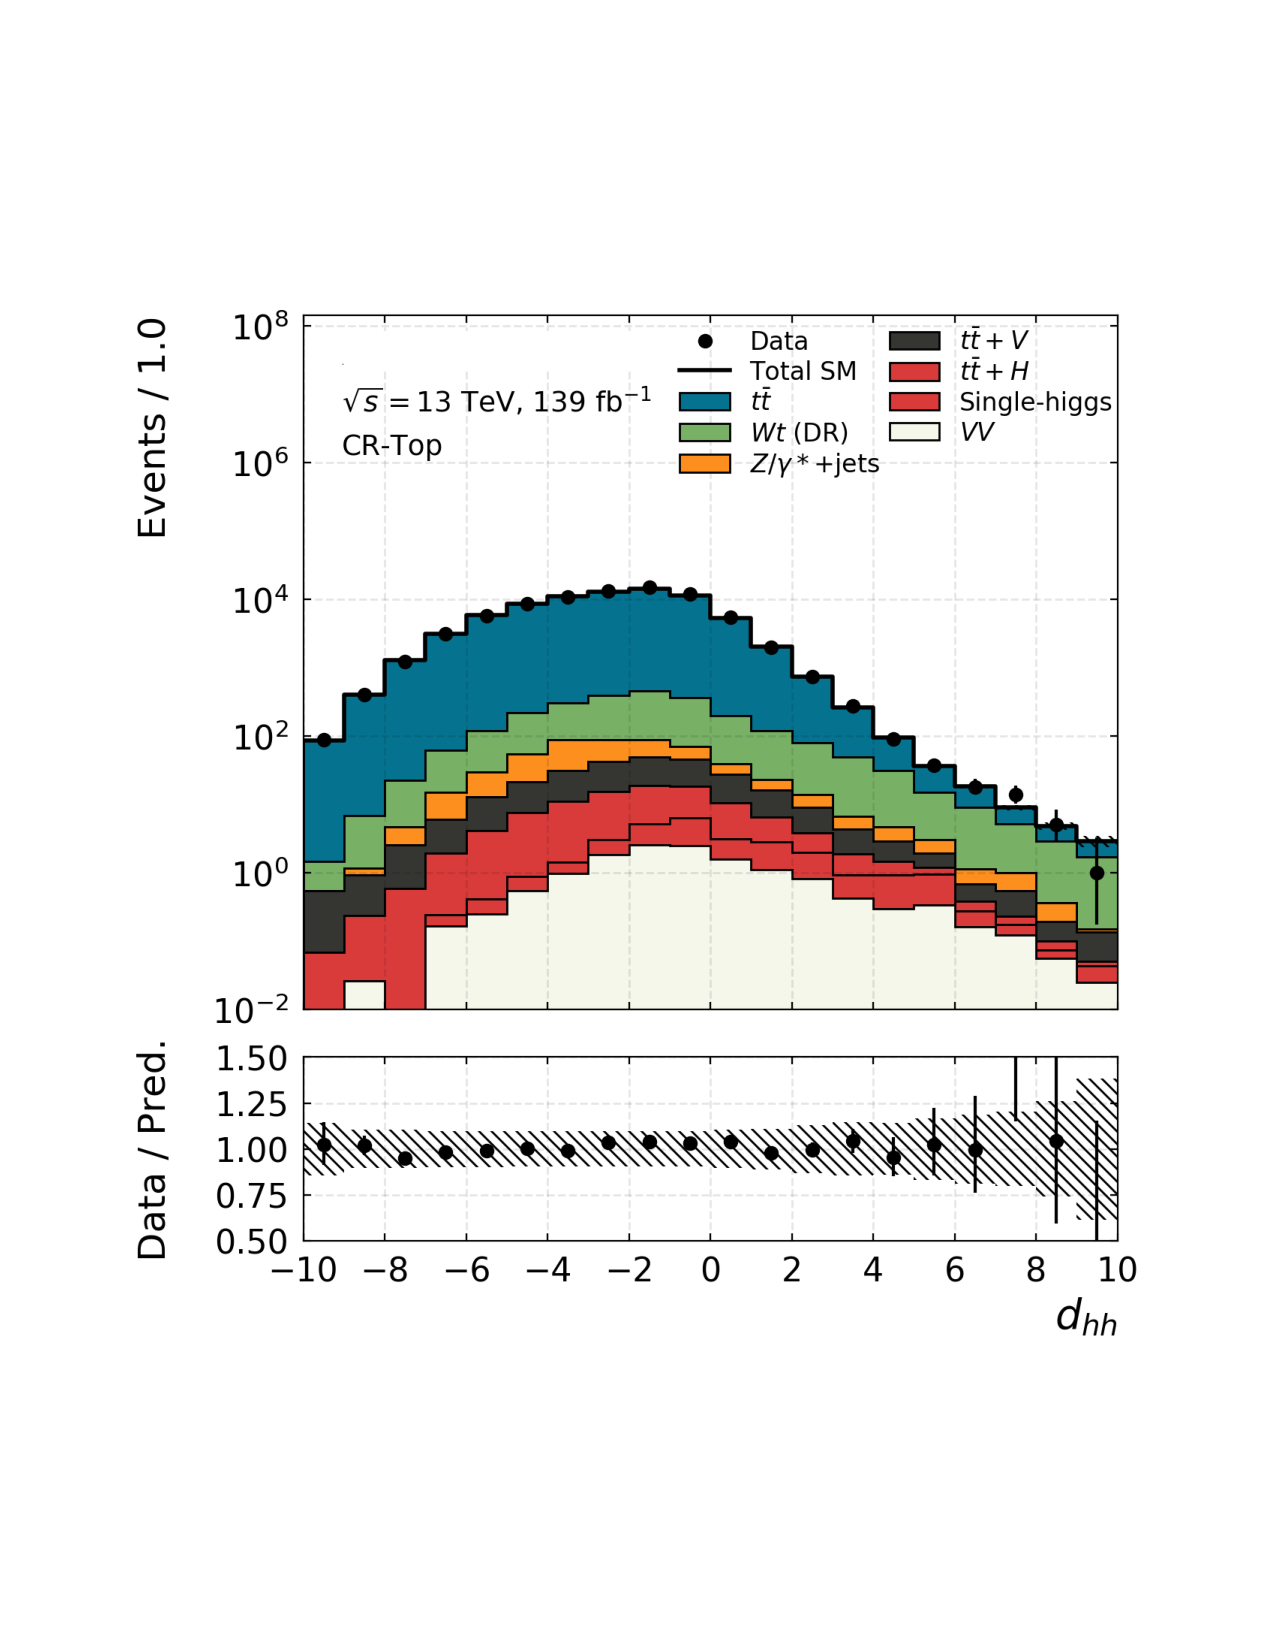
\includegraphics[width=0.65\textwidth]{figures/search_hh/bkg_estimate/crvr/crtop/crtoptest_NN_d_hh_fullsys}
    \caption{
        $d_{hh}$ distribution in the Top control region, CR-Top, without the $d_{hh}$ selection applied.
        The error band in the ratio includes both statistical and systematic uncertainty while
        the error band in the histogram includes only statistically uncertainty.
        The normalization factors obtained from the background-only fit (Table \ref{tab:hh_norm_factors}) are applied
        to the Top (\ttbar~and $Wt$) and $Z$+jets MC processes.
    }
    \label{fig:crtop_nm1_dhh}
\end{figure}

%%%%%%%%%%%%%%%%%%%%%%%%%%%%%%%%%%%%%%%%%%%%%%%%%%%%%%%%%%%%%%%%%%%%%%%%%%%%%%%%%%%
%%%%%%%%%%%%%%%%%%%%%%%%%%%%%%%%%%%%%%%%%%%%%%%%%%%%%%%%%%%%%%%%%%%%%%%%%%%%%%%%%%%
%%%%%%%%%%%%%%%%%%%%%%%%%%%%%%%%%%%%%%%%%%%%%%%%%%%%%%%%%%%%%%%%%%%%%%%%%%%%%%%%%%%
%
% Z+HF
%
%%%%%%%%%%%%%%%%%%%%%%%%%%%%%%%%%%%%%%%%%%%%%%%%%%%%%%%%%%%%%%%%%%%%%%%%%%%%%%%%%%%
%%%%%%%%%%%%%%%%%%%%%%%%%%%%%%%%%%%%%%%%%%%%%%%%%%%%%%%%%%%%%%%%%%%%%%%%%%%%%%%%%%%
%%%%%%%%%%%%%%%%%%%%%%%%%%%%%%%%%%%%%%%%%%%%%%%%%%%%%%%%%%%%%%%%%%%%%%%%%%%%%%%%%%%

\FloatBarrier
\subsection{$Z$ Boson Production in Association with Heavy Flavor Jets}
\label{sec:cr_zhf}

In the $\ge 2$ $b$-tagged jet regions of phase space that are being probed by SR-SF and SR-DF (c.f. Table~\ref{tab:hh_sr_def}),
there remains non-negligible contamination from $Z$+jets processes.
As the cross-section of $Z$-boson production in association with heavy flavor jets is known to be mismodelled
by MC predictions~\cite{Chatrchyan:2013zja,Aad:2014dvb}, especially in the relatively
collinear $b$-tagged jet regimes sensitive to the theoretically challenging $g \rightarrow bb$ processes
that $h \rightarrow bb$ analyses are probing, we define a CR and VR enriched in the
$Z$+heavy-flavor processes in order to constrain the MC prediction with data.

We define the $Z$+heavy-flavor process as those $Z$-boson processes whose leading two $b$-tagged
jets are identified as arising either from $b$- or $c$-hadrons, using the MC truth-level information
to identify the jets as such.
The corresponding definitions of the $Z$+heavy-flavor and $Z$+light-flavor processes are given
in Table~\ref{tab:zhf_def}.

\begin{table}[!htb]
    \begin{center}
        \caption{
            Definition of the $Z$+heavy-flavor and $Z$+light-flavor backgrounds.
            Shown are the truth-level association of the leading two reconstruction level $b$-tagged
            jets (in MC) to $b$- or $c$-hadrons or light-flavor processes (mis-tags), indicated
            by $\ell$.
        }        
        \label{tab:zhf_def}
        \begin{tabular}{l|c}
        \hline
        \hline
            \textbf{Process} & \textbf{Truth-level $b$-tagged Jet Pair Origin} \\
            \hline
            $Z$+heavy-flavor & $bb$, $bc$, or $cc$ \\
            $Z$+light-flavor & $b \ell$, $c \ell$ or $\ell \ell$ \\
        \hline
        \hline
        \end{tabular}
    \end{center}
\end{table}

The $Z$+heavy-flavor regions are inclusive in dilepton flavor and are defined by inverting the $m_{\ell \ell} < 60$ GeV
requirement made in the SRs.
The $Z$+heavy-flavor CR, CR-Z+HF, selects events on the $Z$-boson mass pole with a relatively
tight window in $m_{\ell \ell}$ centered at $m_Z = 91.2$\,\GeV.
The $Z$+heavy-flavor VR, VR-Z+HF, selects events in side-bands of $m_{\ell \ell}$ around the window
selected by CR-Z+HF.
Both CR-Z+HF and VR-Z+HF retain the requirements on the $b$-tagged jets that are applied in the SRs,
so as to ensure that the $b$-tagged jet kinematics between these regions are similar.
As with CR-Top and VR-Top, the requirement on \dhh is relaxed in order to increase
the statistics available for these regions.
Independent studies have been performed to study the dependence of the $Z$+heavy-flavor normalisation correction
factor derived in CR-Z+HF on the \dhh selection, showing that there is no statistically significant
dependence on the cut. The loose \dhh selection is therefore adequate and allows for improved statistical
precision in the definition of the $Z$+heavy-flavor process' normalization correction.

Figures~\ref{fig:crz_kin_plots_0}-\ref{fig:crz_kin_plots_2} show distributions of the relevant
observables in CR-Top.
Figure~\ref{fig:crz_nm1_dhh} shows the distribution of the composite discriminant \dhh in CR-Top
without the requirement on \dhh applied, so that the full shape of the discriminant may be studied.

\begin{table}[!htb]
    \begin{center}
        \caption{
            Definitions of the CR and VR for the $Z$+heavy flavor process
            for the search targeting the dilepton $hh \rightarrow \bbww$ process.
        }
        \label{tab:hh_crzhf}
        \begin{tabular}{l | c c}
        \hline
        \hline
                & \multicolumn{2}{c}{\textbf{Region}} \\
            \cline{2-3}
            \textbf{Observable} & \textbf{CR-Z+HF} & \textbf{VR-Z+HF} \\
            \hline
            Dilepton Flavor & $ee, \mu\mu, e \mu,$ or $\mu e$ & $ee$ or $\mu\mu$ \\
            $b$-tagged jet multiplicity & $\ge 2$ & $\ge 2$ \\
            $m_{bb}$ [GeV] & $\in [110, 140]$ & $\in [110, 140]$ \\
            $m_{\ell \ell}$ [GeV] & $\in [81.2, 101.2]$ & $\in[71.2, 81.2]$ or $\in [101.2, 115]$ \\
            \dhh & $>0$ & $>0$ \\
        \hline
        \hline
        \end{tabular}
    \end{center}
\end{table}

\begin{figure}[!htb]
    \centering
    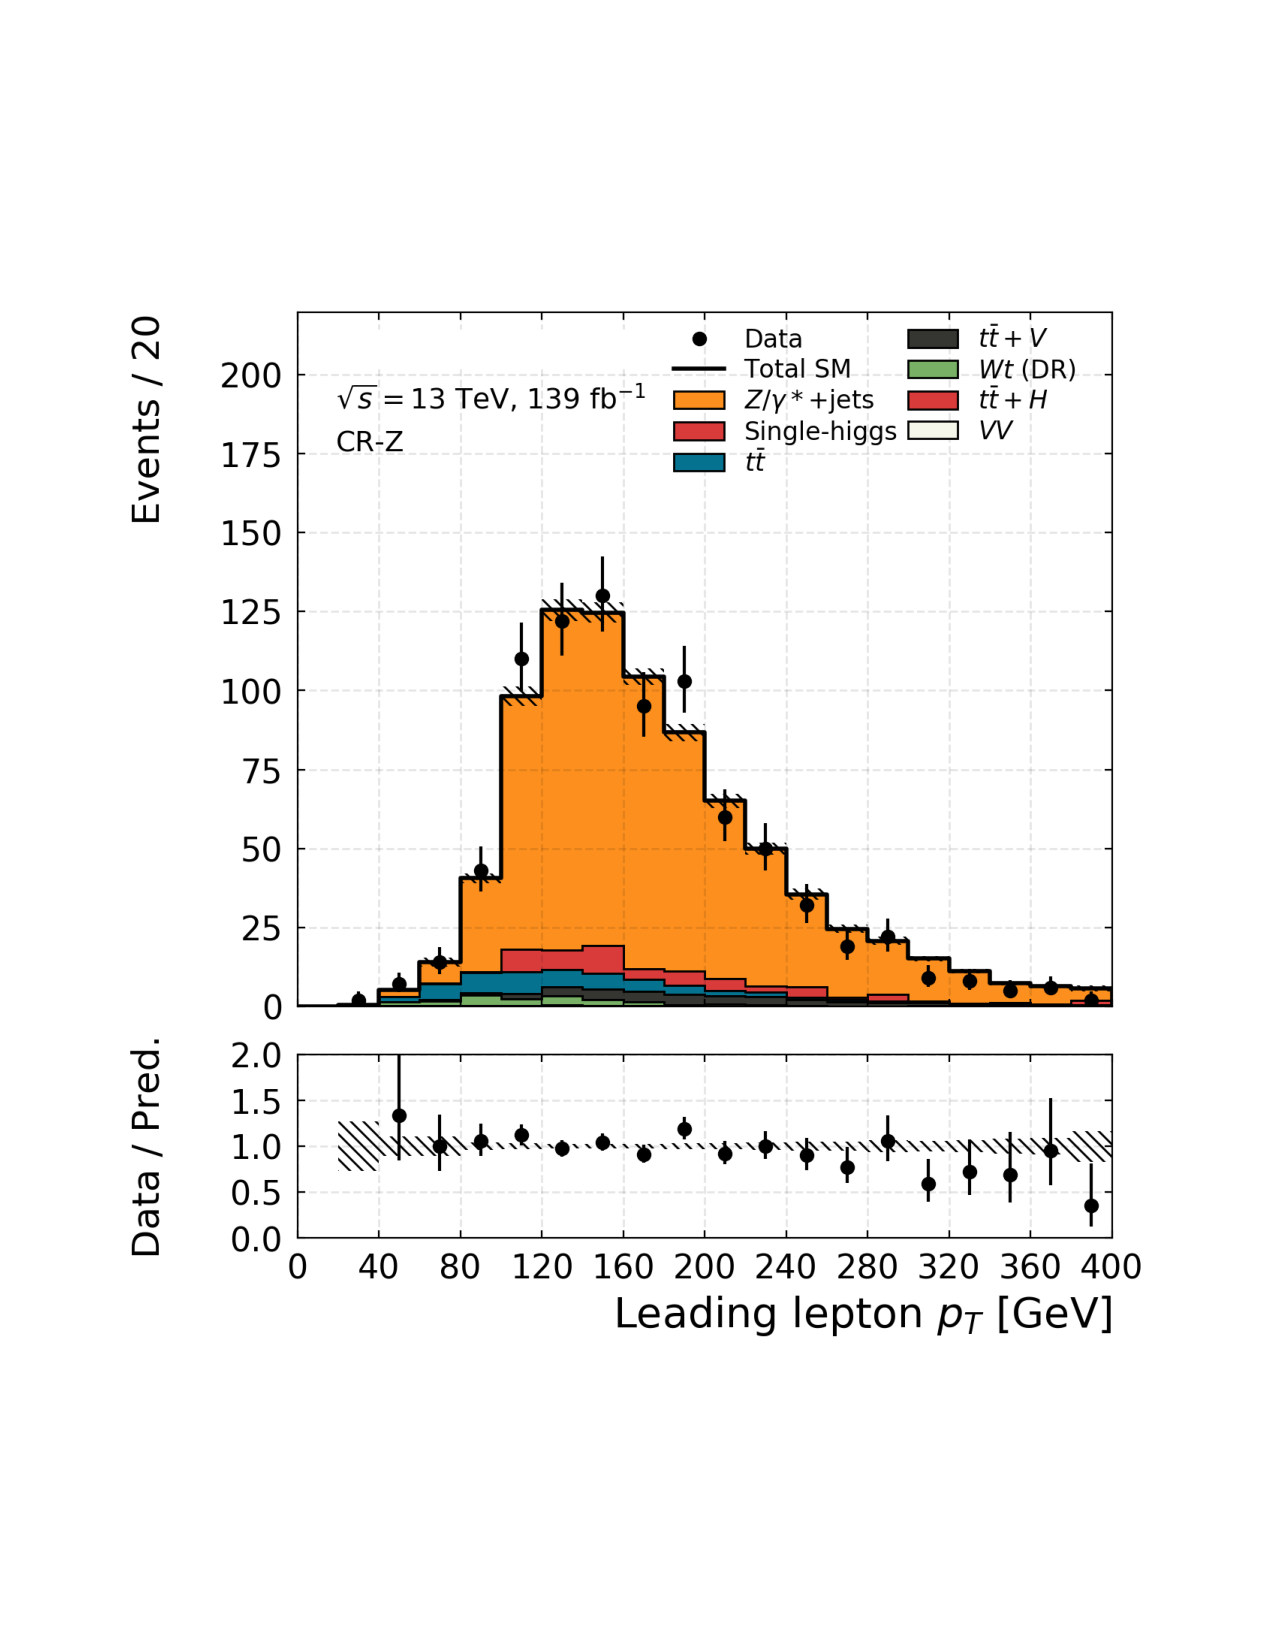
\includegraphics[width=0.4\textwidth]{figures/search_hh/bkg_estimate/crvr/crzhf/crztest_l0_pt}
    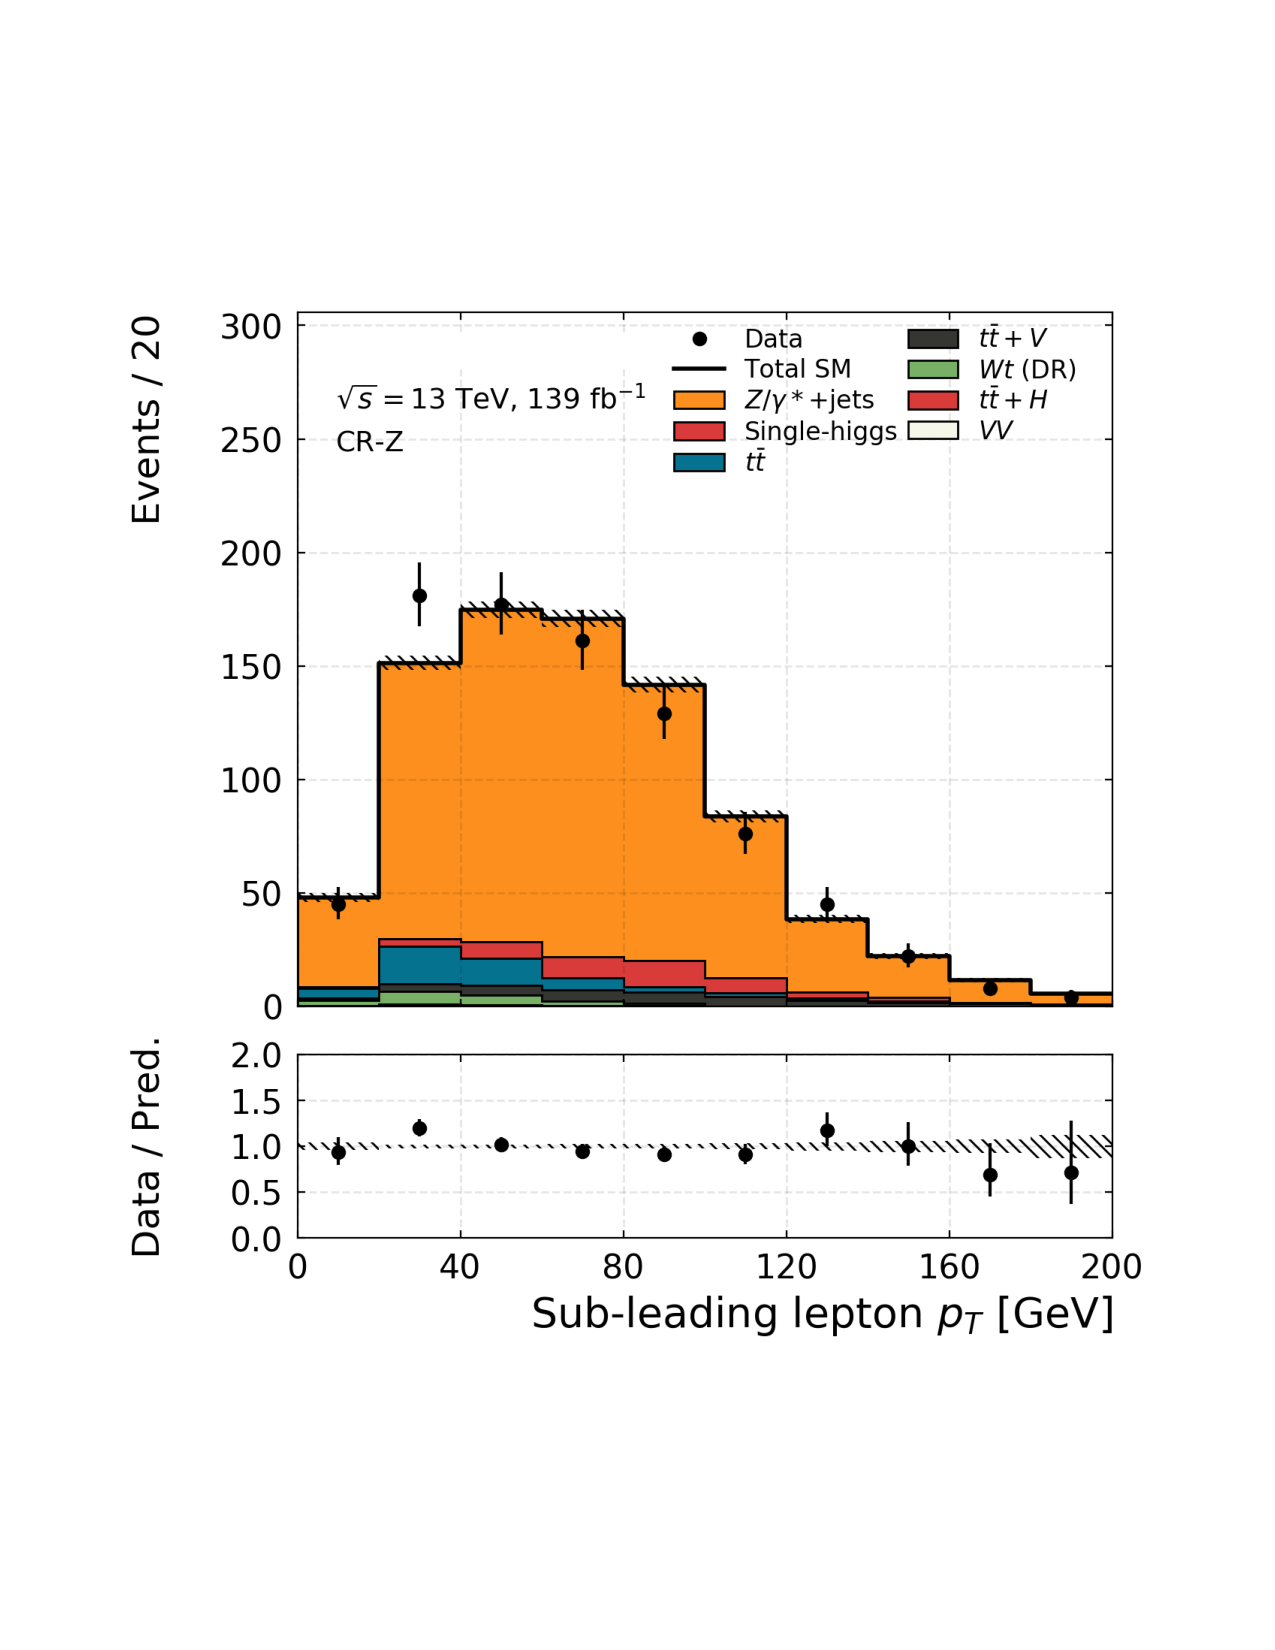
\includegraphics[width=0.4\textwidth]{figures/search_hh/bkg_estimate/crvr/crzhf/crztest_l1_pt}
    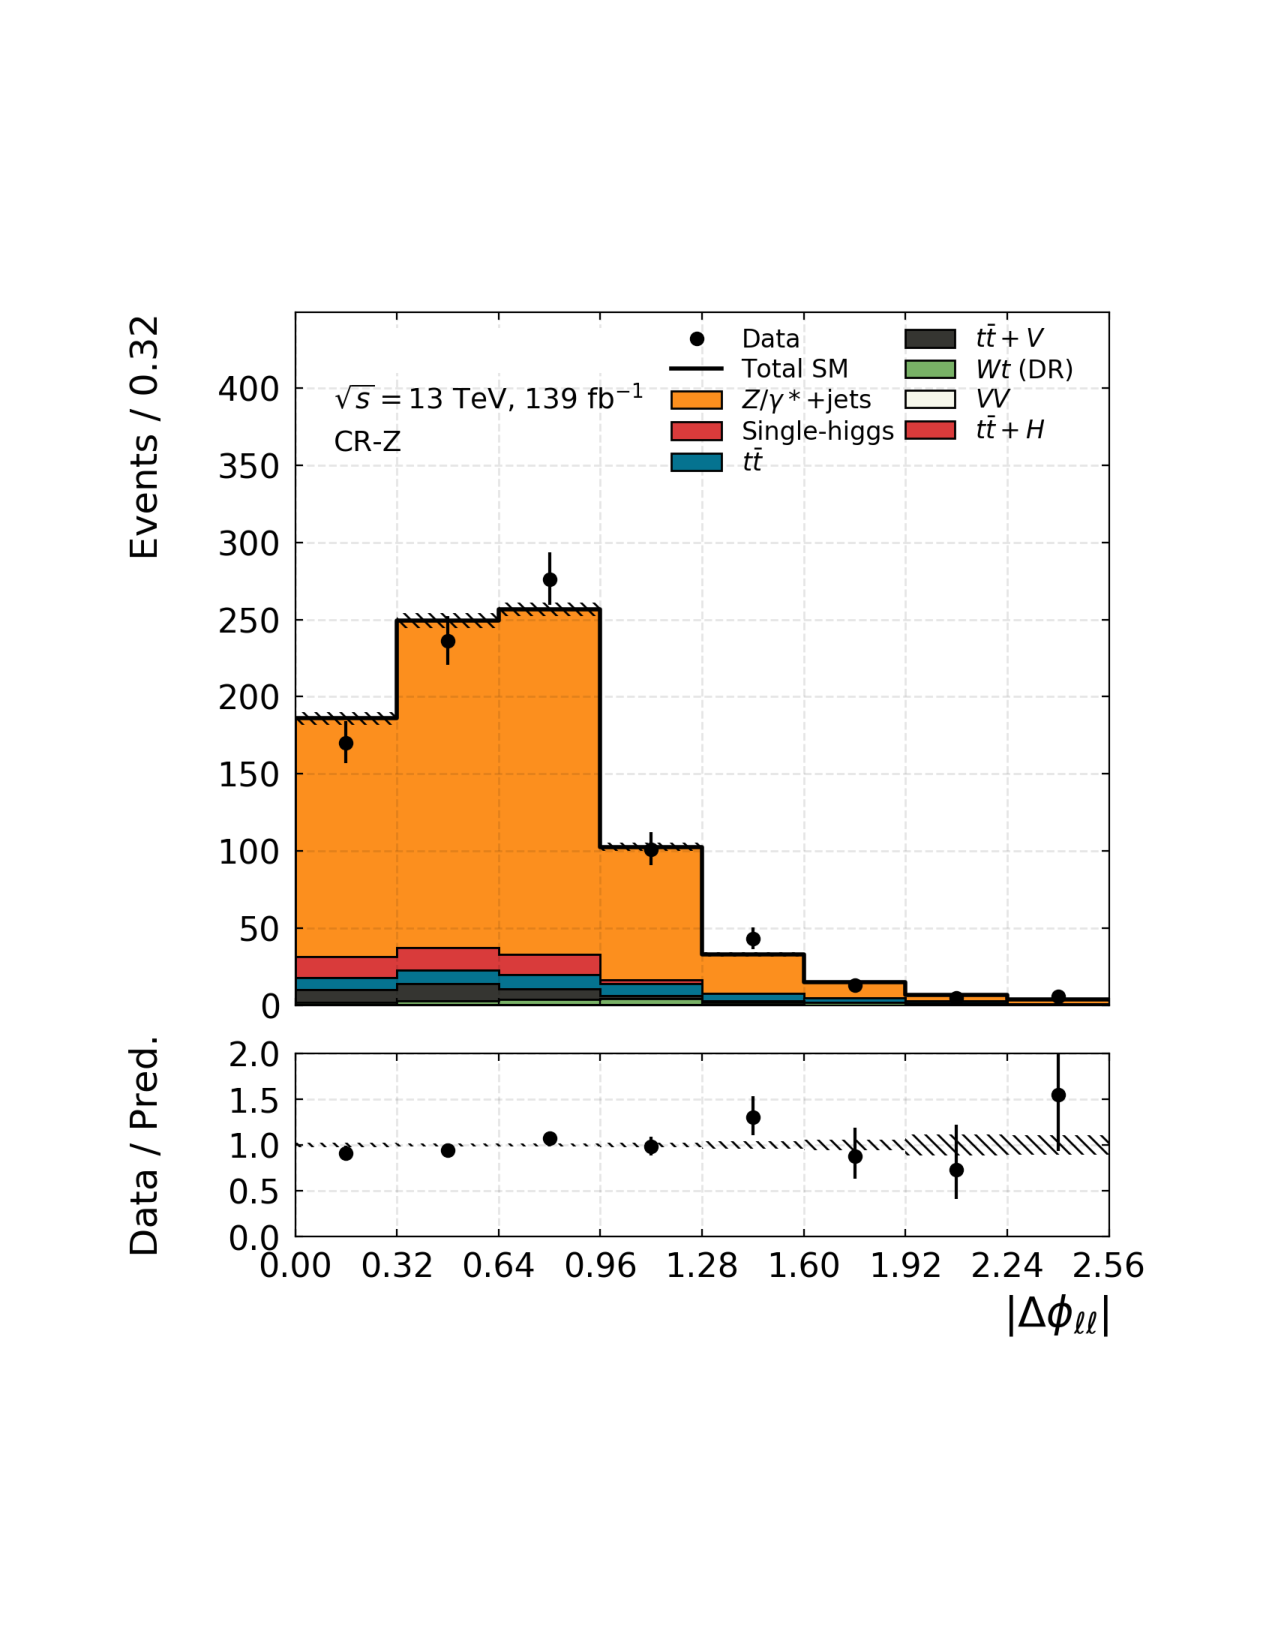
\includegraphics[width=0.4\textwidth]{figures/search_hh/bkg_estimate/crvr/crzhf/crztest_dphi_ll}
    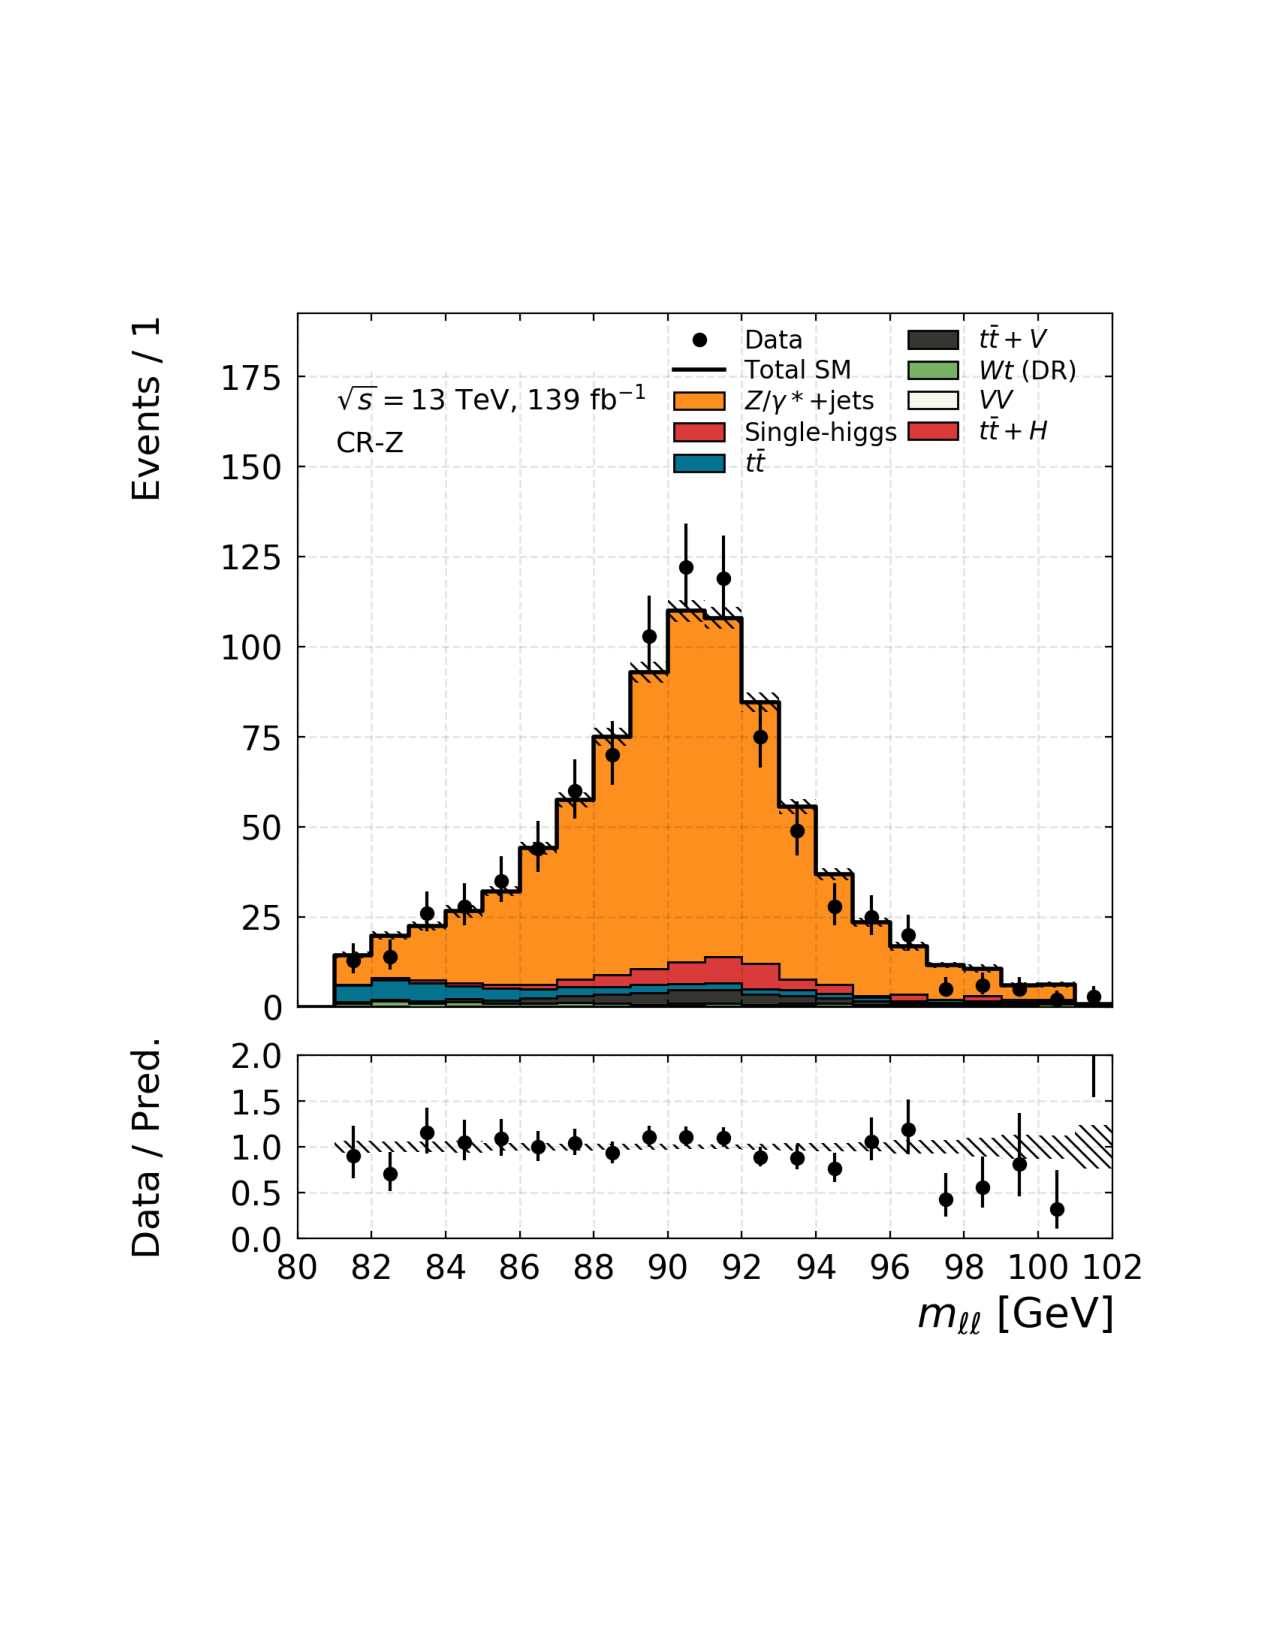
\includegraphics[width=0.4\textwidth]{figures/search_hh/bkg_estimate/crvr/crzhf/crztest_mll}
    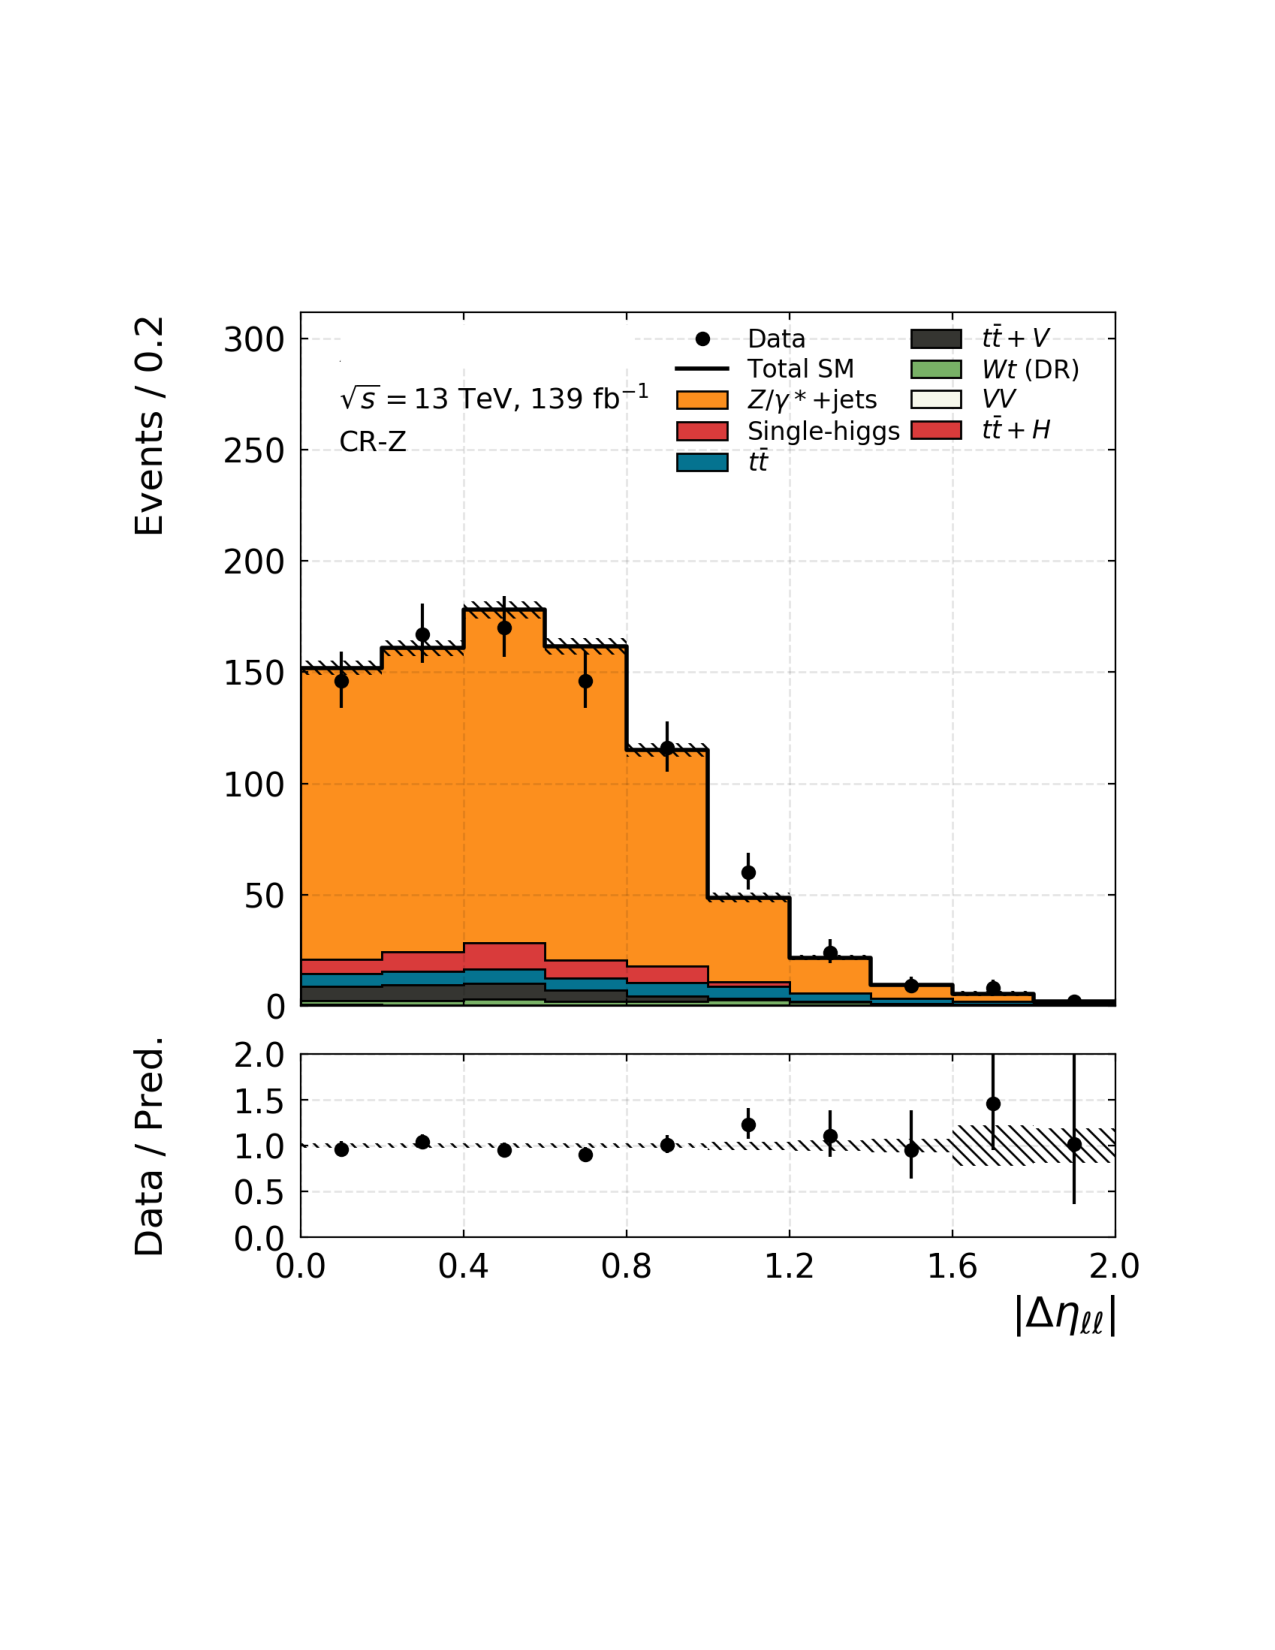
\includegraphics[width=0.4\textwidth]{figures/search_hh/bkg_estimate/crvr/crzhf/crztest_deta_ll}
    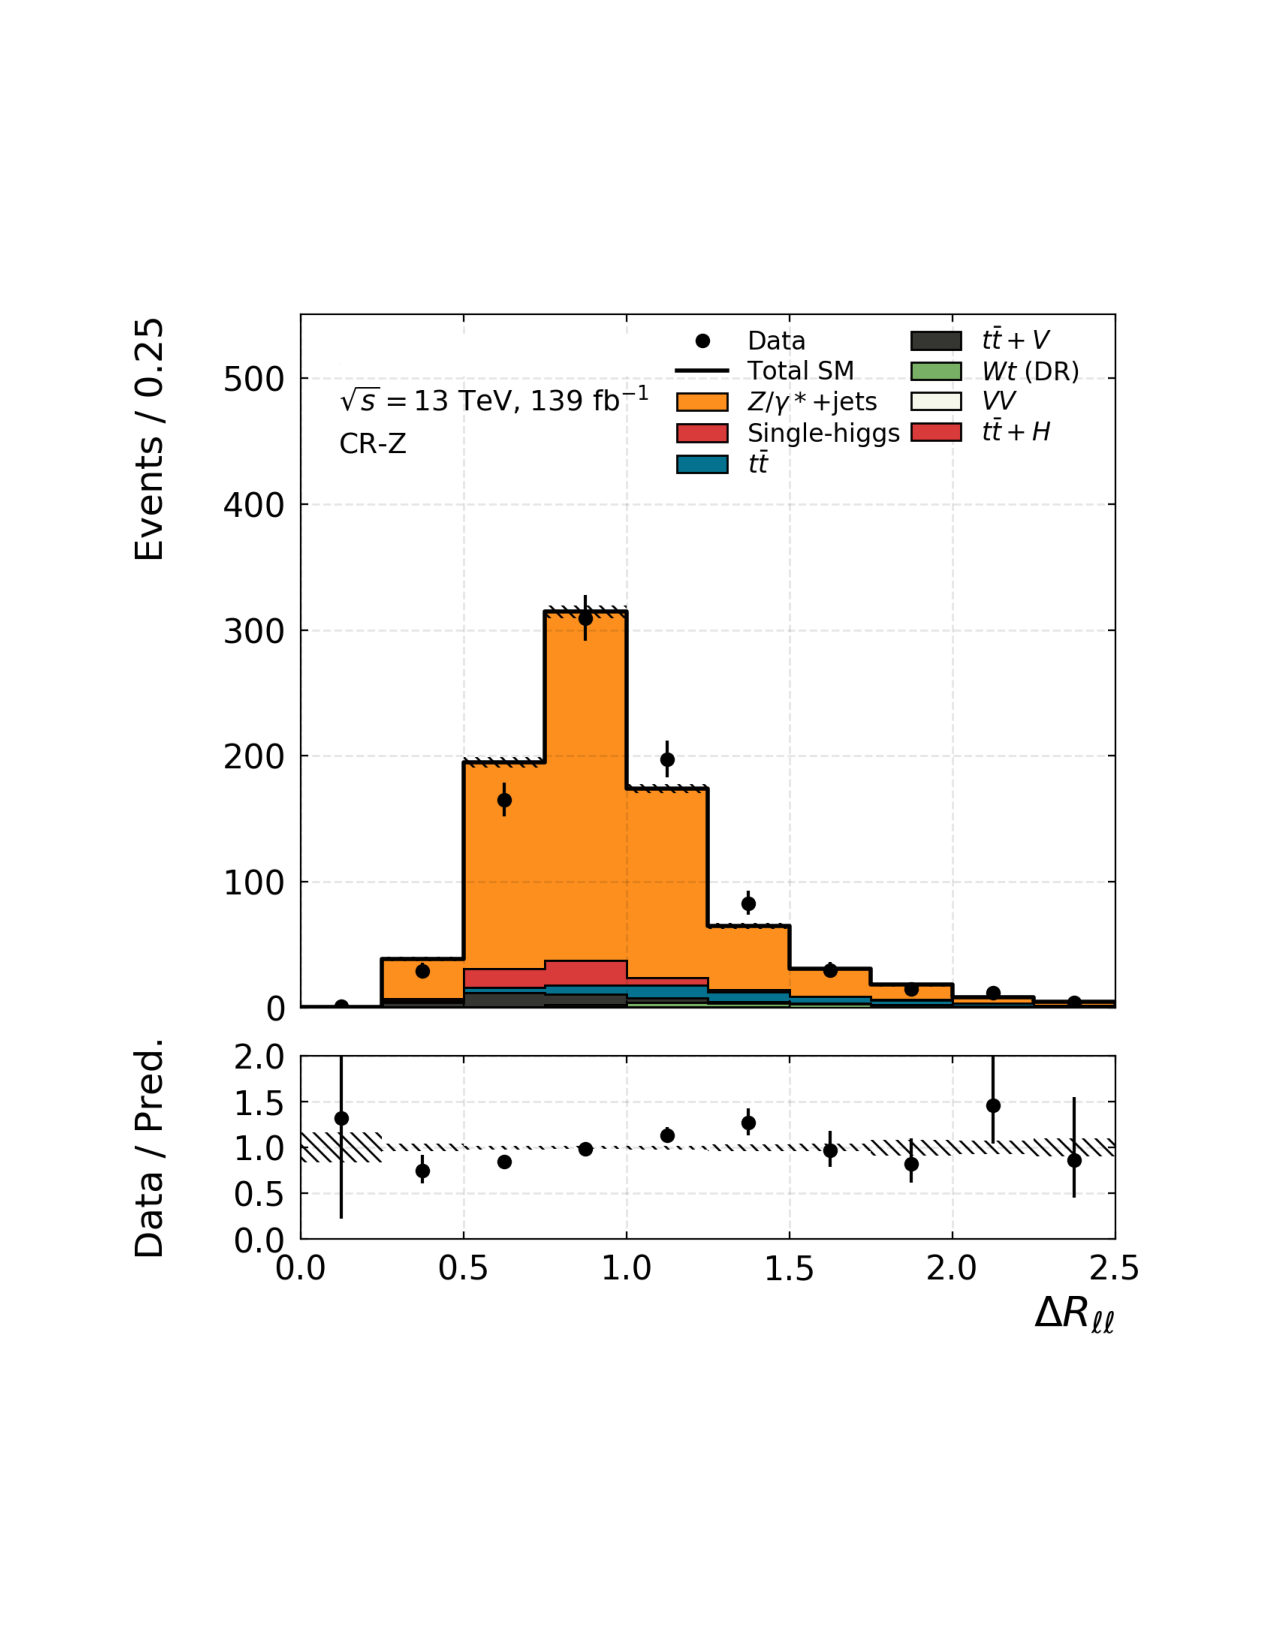
\includegraphics[width=0.4\textwidth]{figures/search_hh/bkg_estimate/crvr/crzhf/crztest_dRll}
    \caption{
    Kinematic distributions in the $Z$+heavy flavor control region, CR-Z+HF.
    The error bands include only the statistical uncertainty.
    The normalization factors obtained from the background-only fit (Table \ref{tab:hh_norm_factors}) are applied
    to the Top (\ttbar~and $Wt$) and $Z$+jets MC processes.
    }
    \label{fig:crz_kin_plots_0}
\end{figure}

\begin{figure}[!htb]
    \centering
    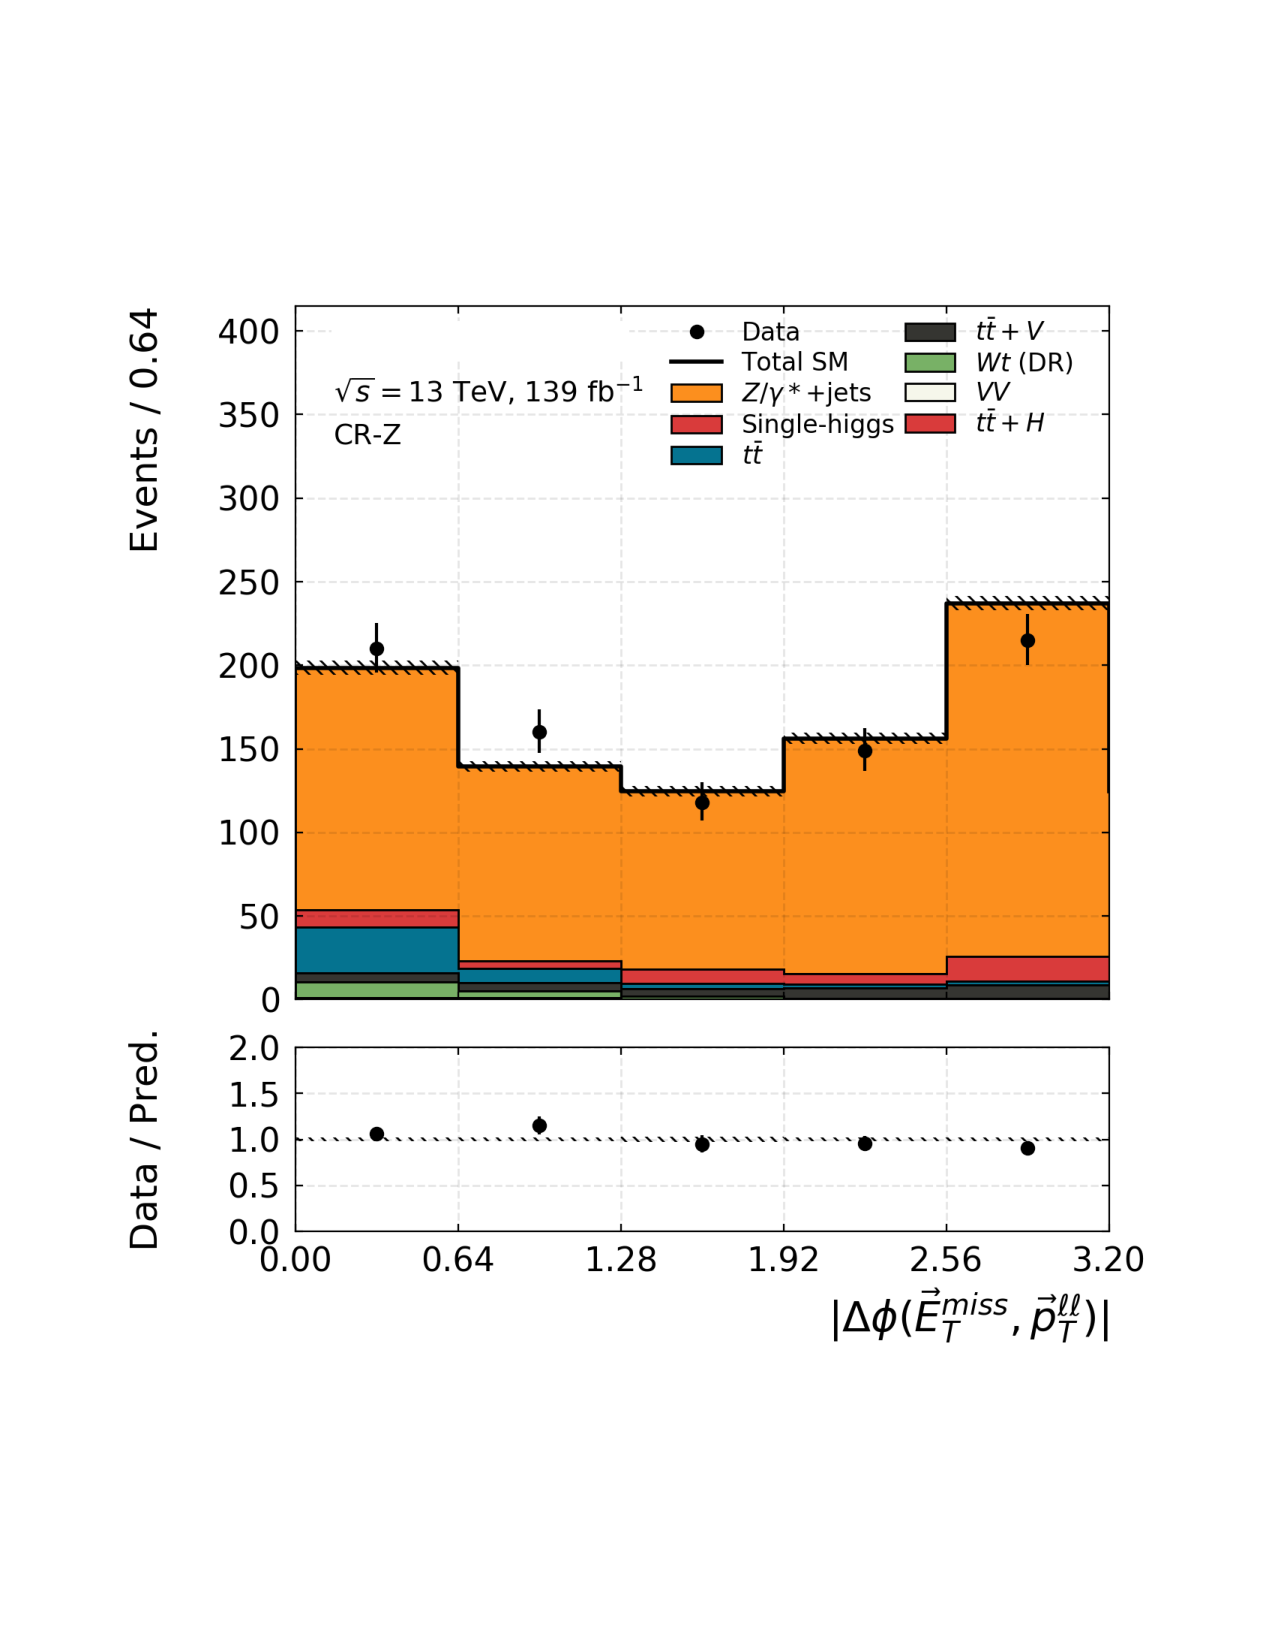
\includegraphics[width=0.4\textwidth]{figures/search_hh/bkg_estimate/crvr/crzhf/crztest_dphi_met_ll}
    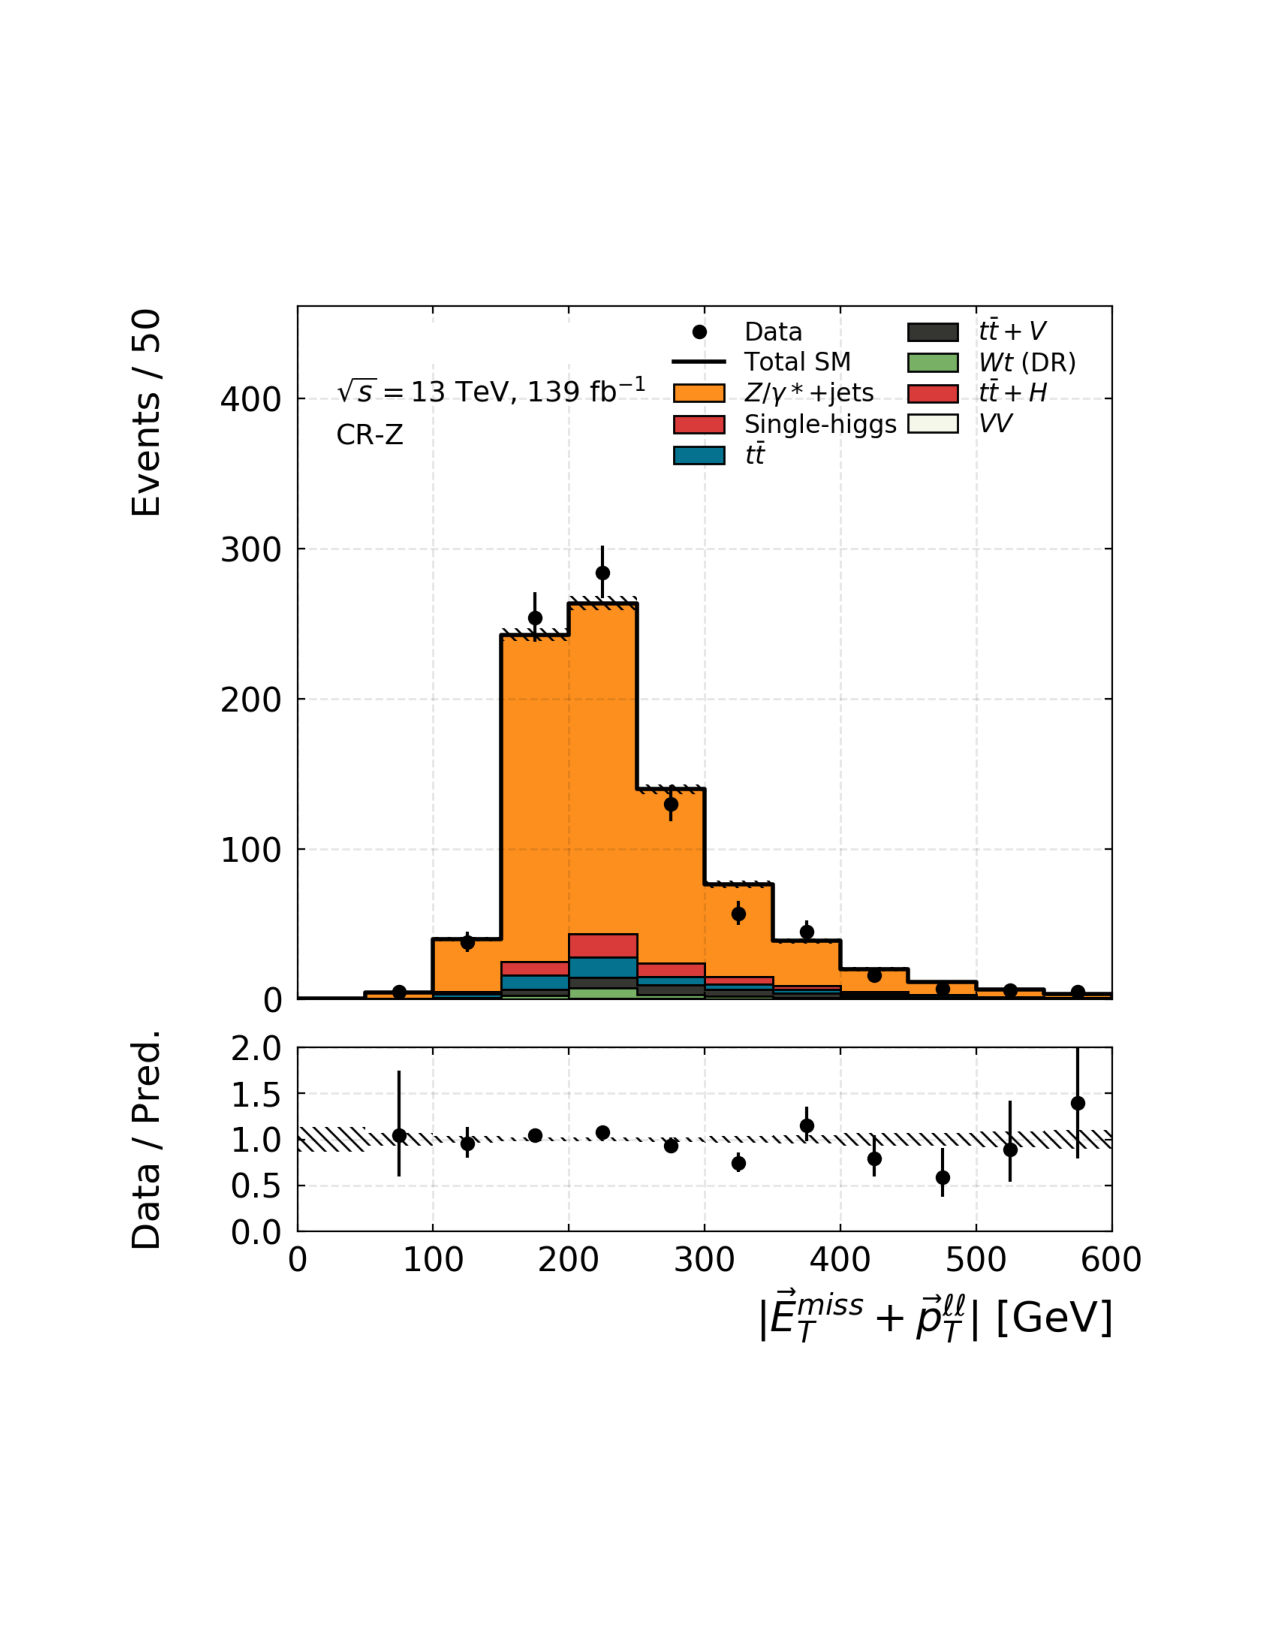
\includegraphics[width=0.4\textwidth]{figures/search_hh/bkg_estimate/crvr/crzhf/crztest_met_pTll}
    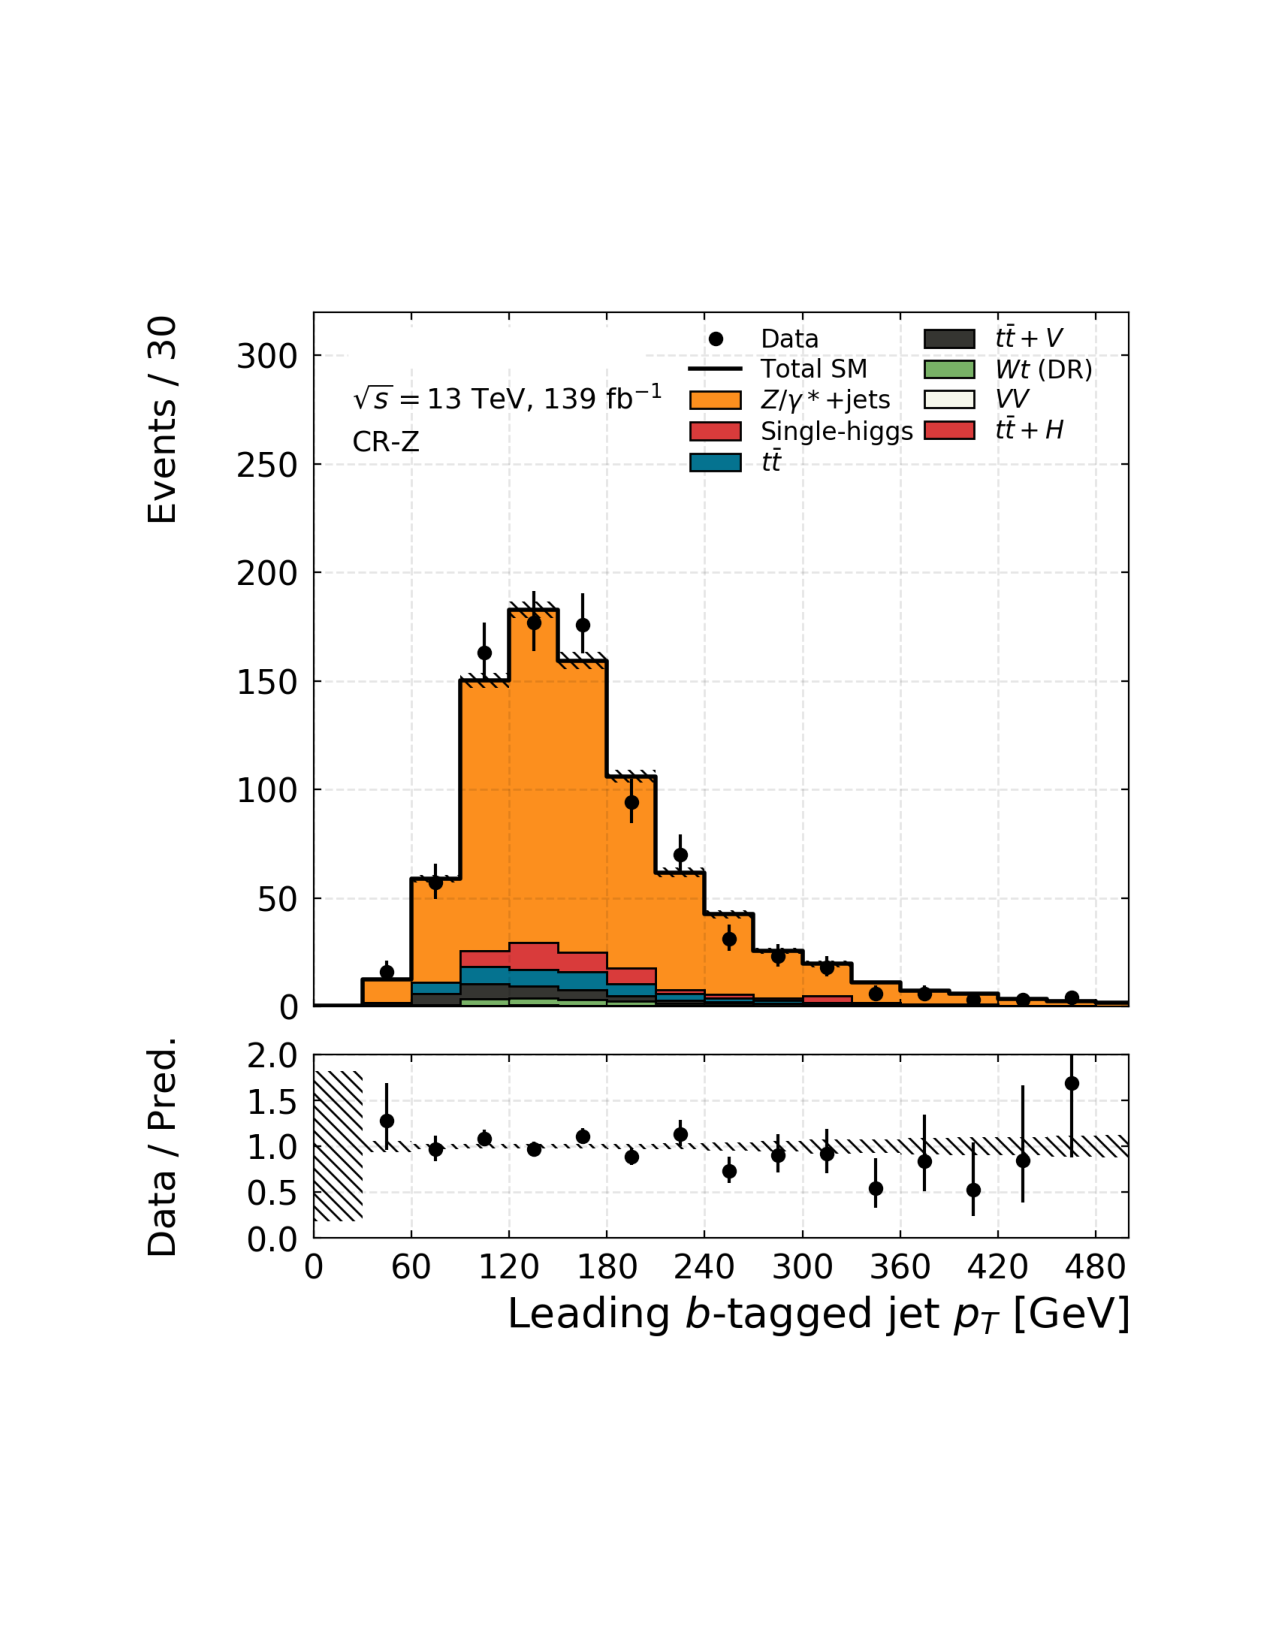
\includegraphics[width=0.4\textwidth]{figures/search_hh/bkg_estimate/crvr/crzhf/crztest_bj0_pt}
    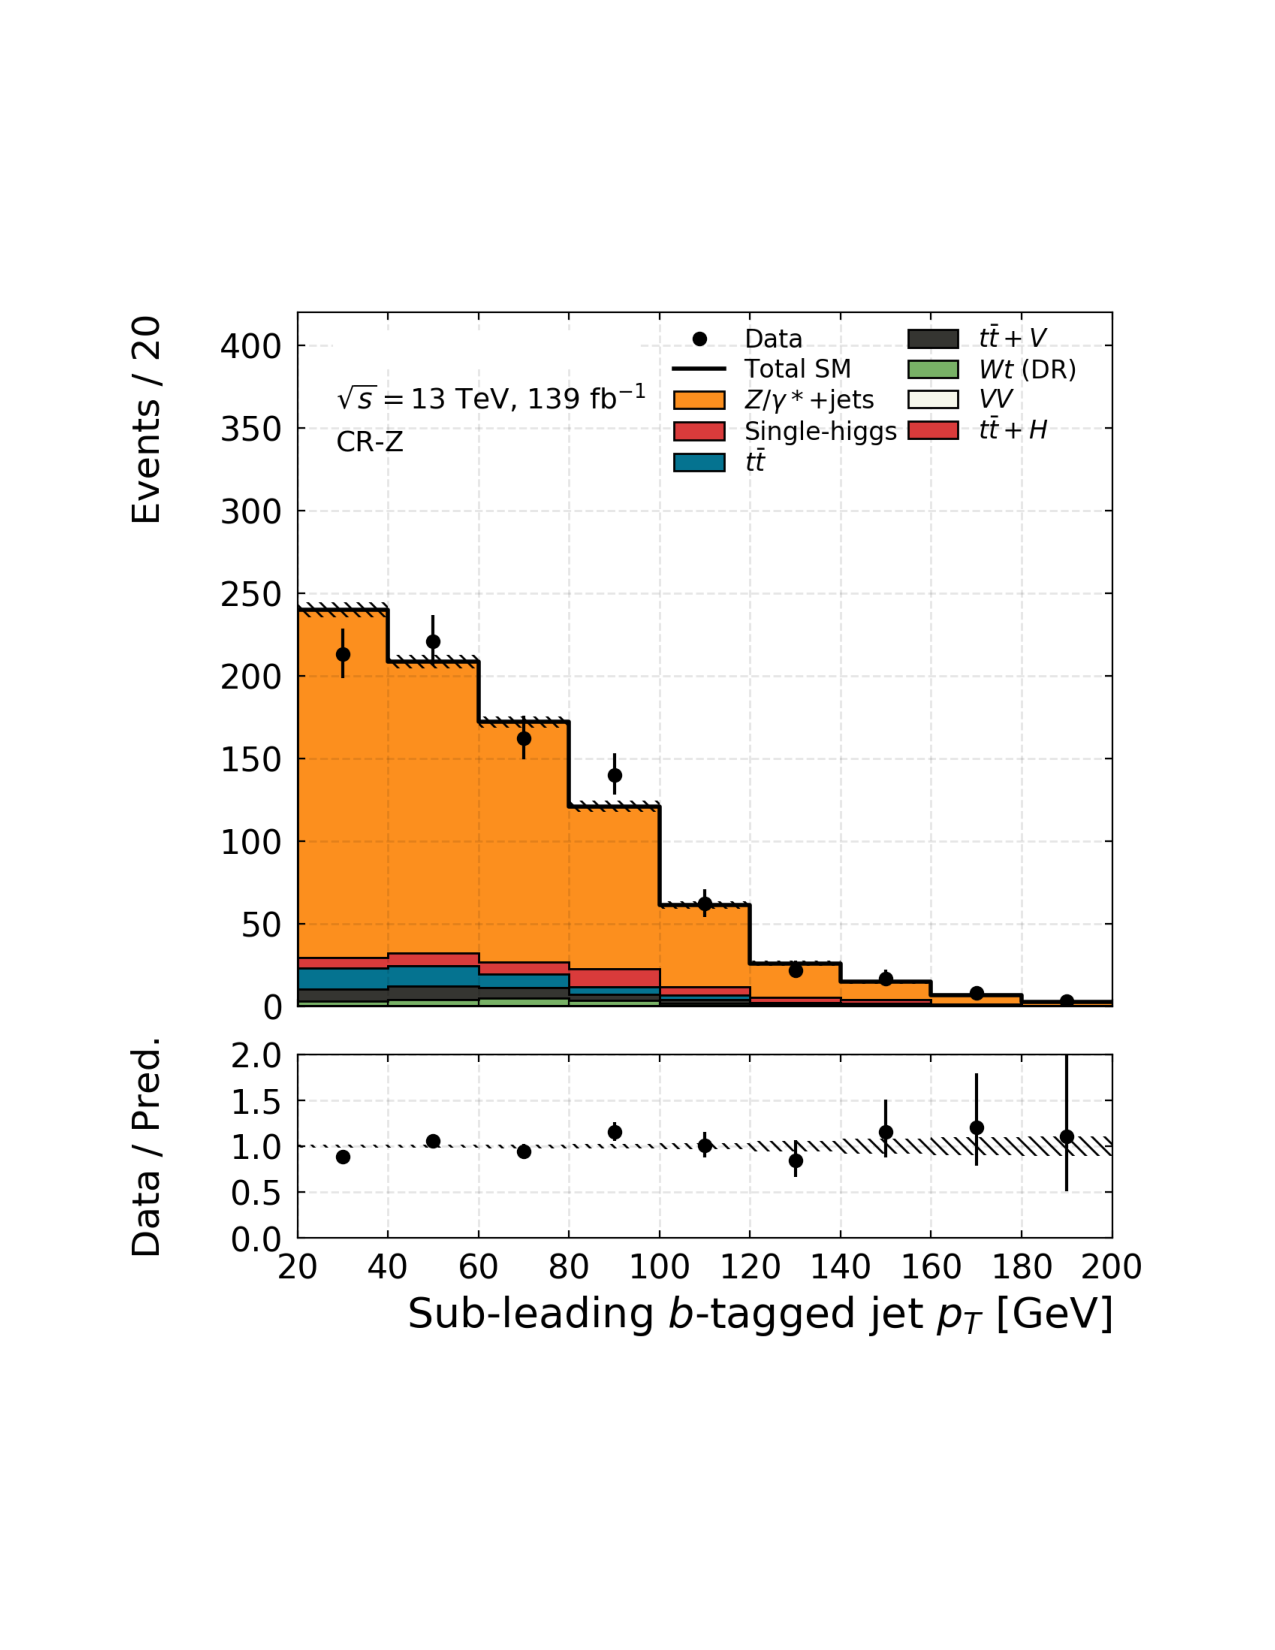
\includegraphics[width=0.4\textwidth]{figures/search_hh/bkg_estimate/crvr/crzhf/crztest_bj1_pt}
    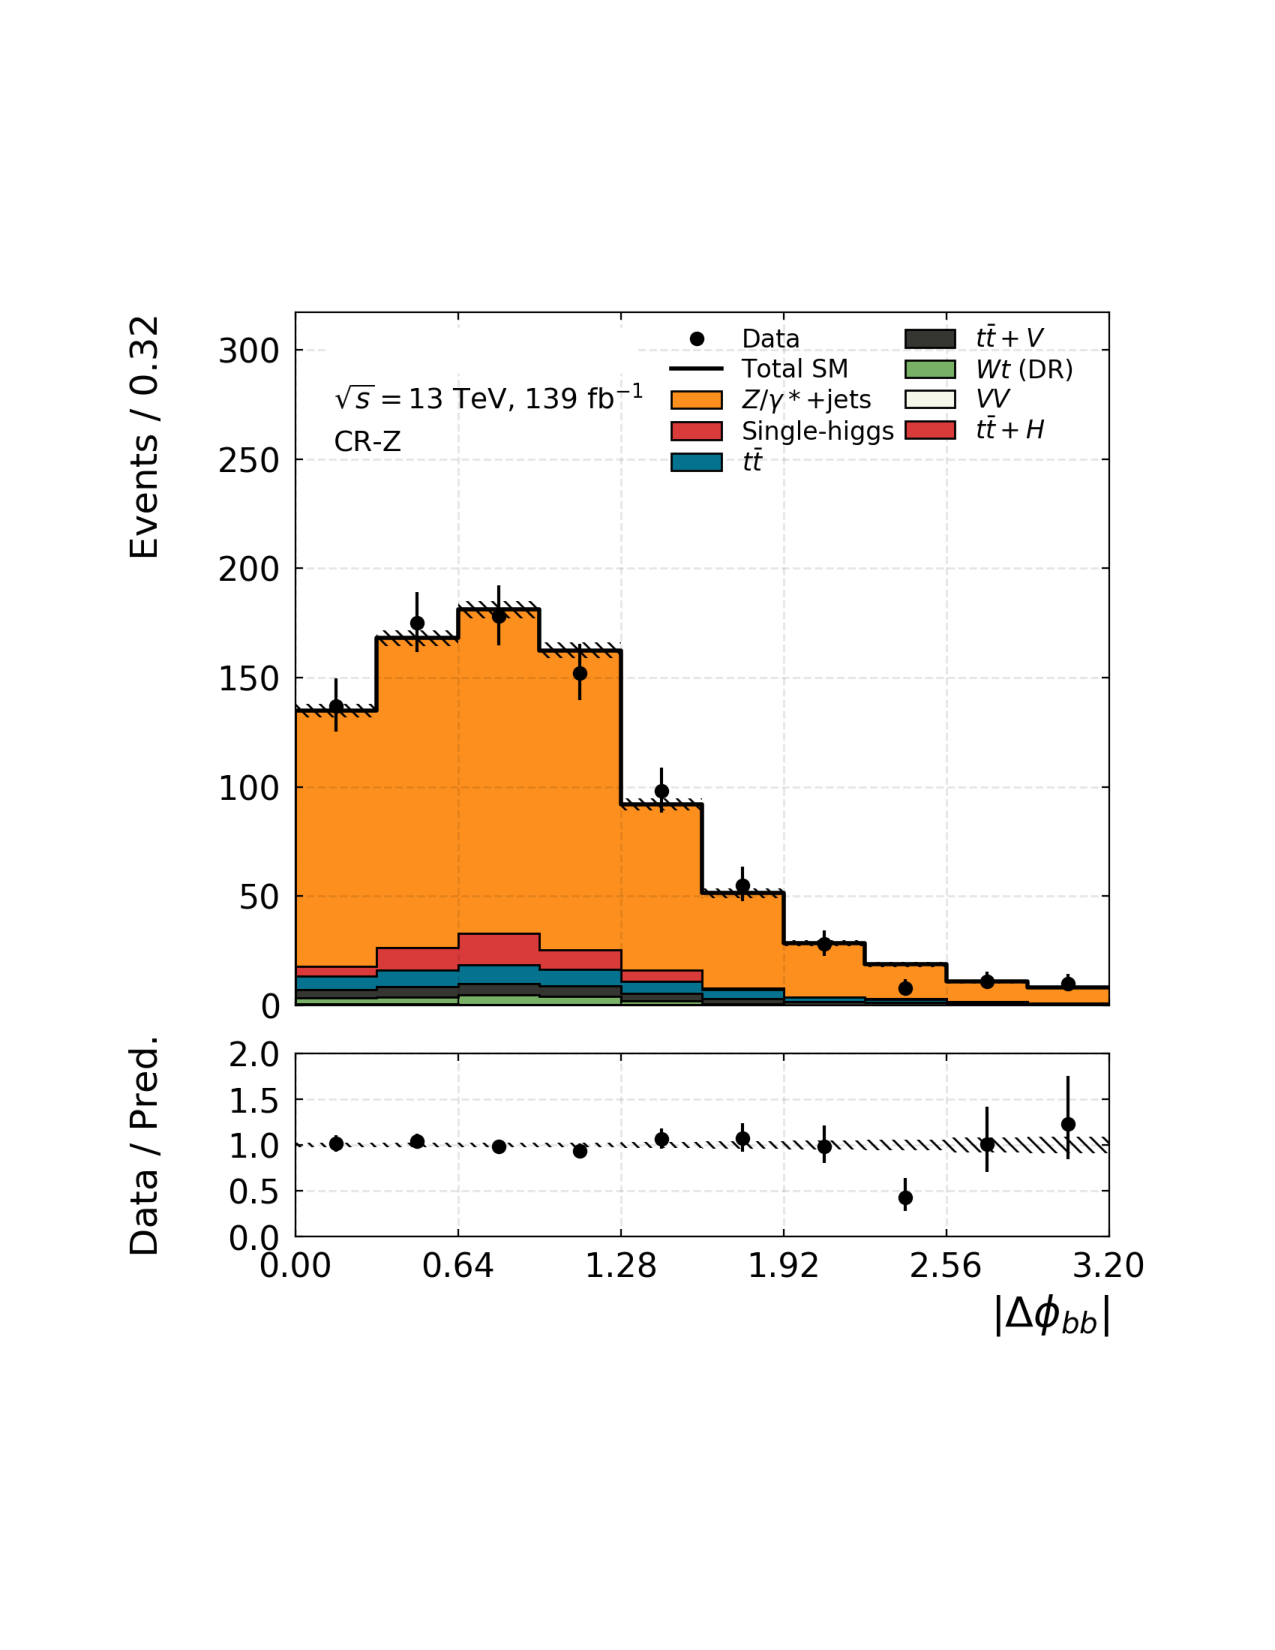
\includegraphics[width=0.4\textwidth]{figures/search_hh/bkg_estimate/crvr/crzhf/crztest_dphi_bb}
    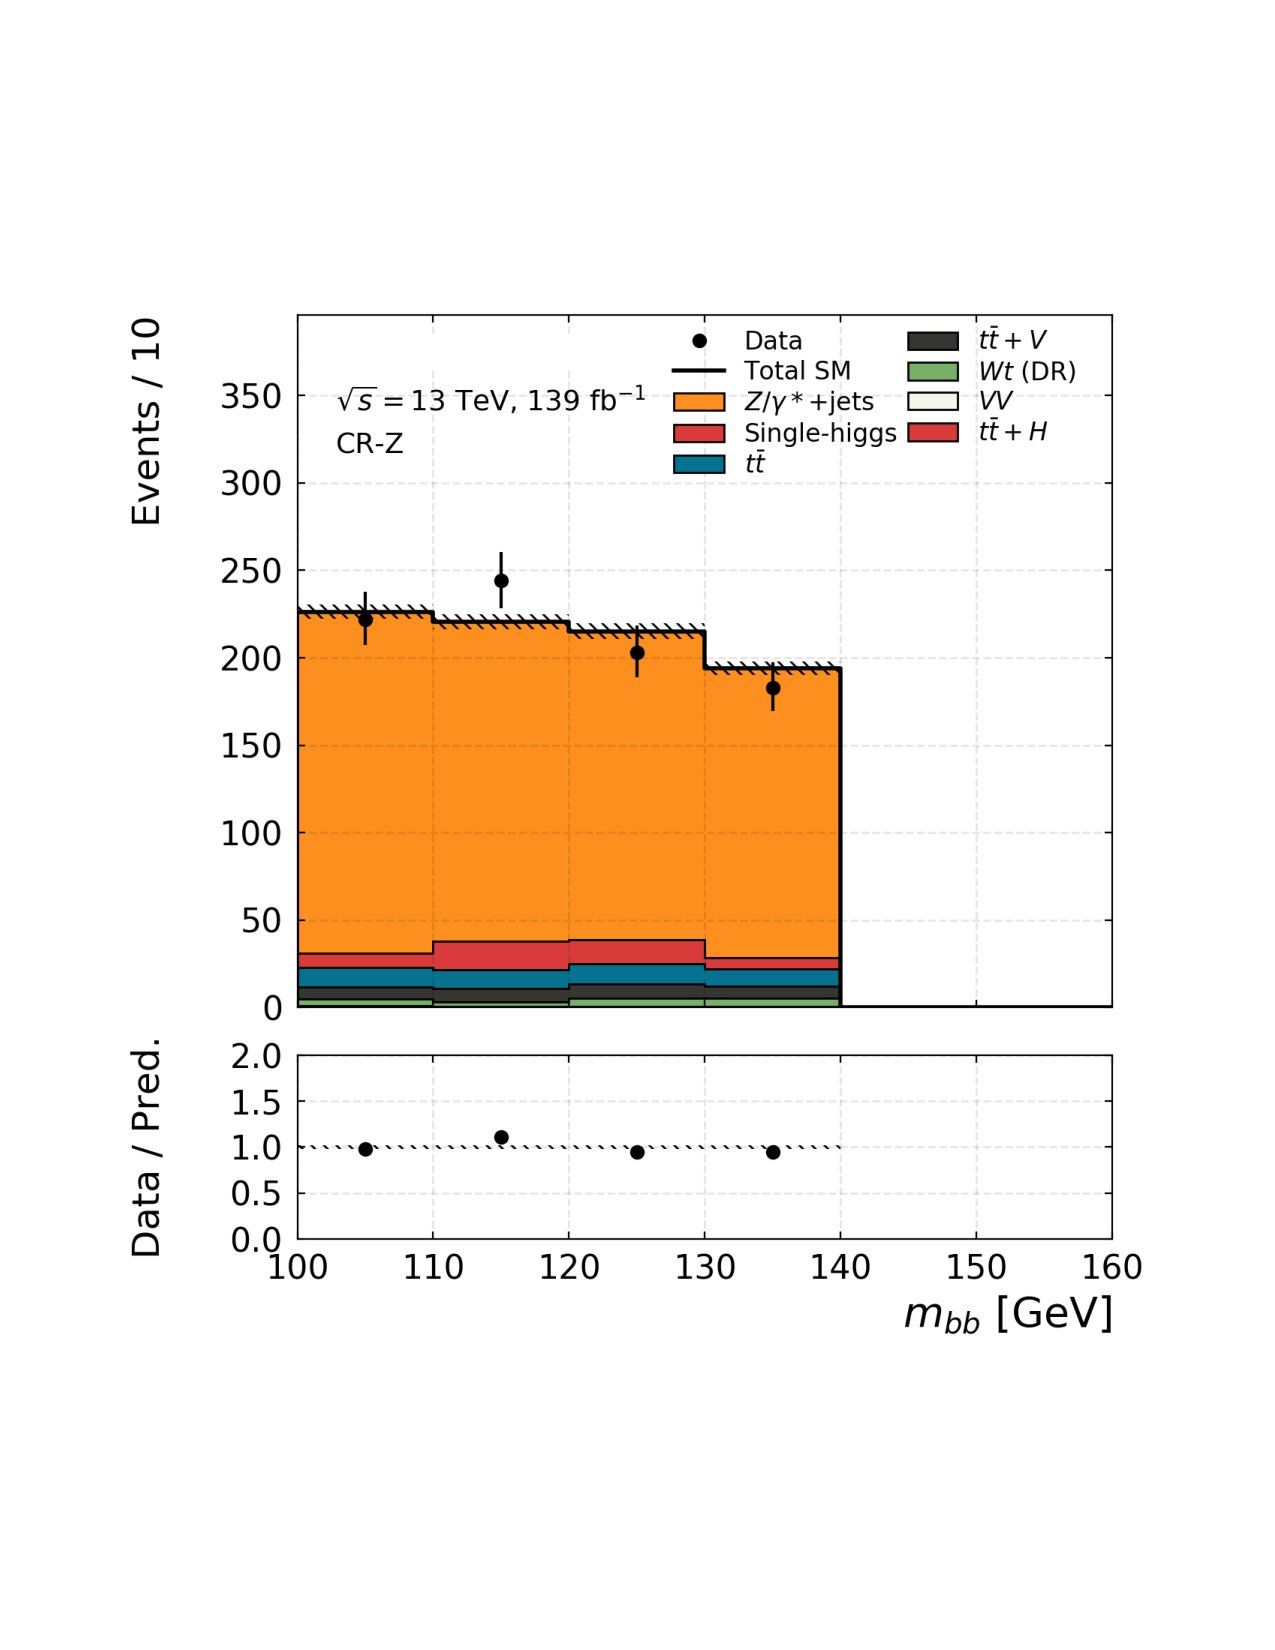
\includegraphics[width=0.4\textwidth]{figures/search_hh/bkg_estimate/crvr/crzhf/crztest_mbb}
    \caption{
    Kinematic distributions in the $Z$+heavy flavor control region, CR-Z+HF.
    The error bands include only the statistical uncertainty.
    The normalization factors obtained from the background-only fit (Table \ref{tab:hh_norm_factors}) are applied
    to the Top (\ttbar~and $Wt$) and $Z$+jets MC processes.
    }
    \label{fig:crz_kin_plots_1}
\end{figure}
\begin{figure}[!htb]
    \centering
    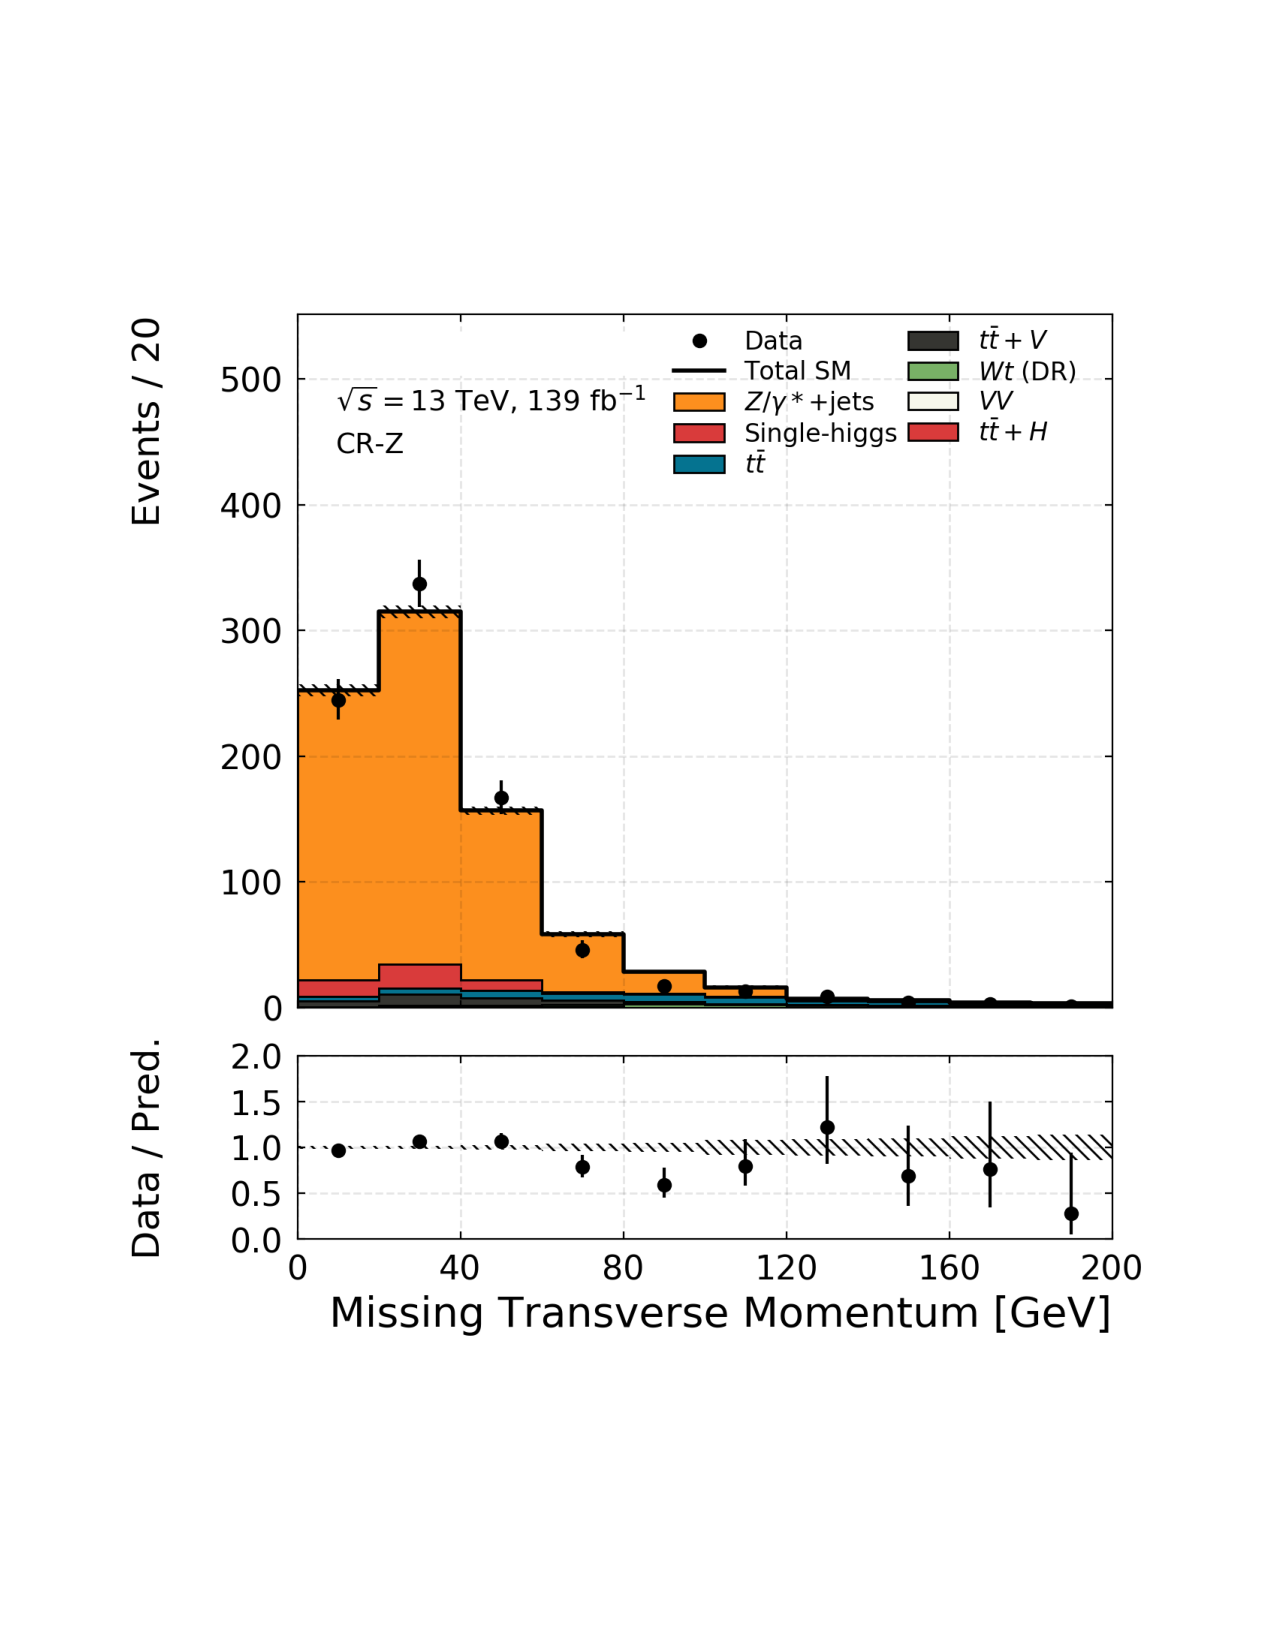
\includegraphics[width=0.4\textwidth]{figures/search_hh/bkg_estimate/crvr/crzhf/crztest_met}
    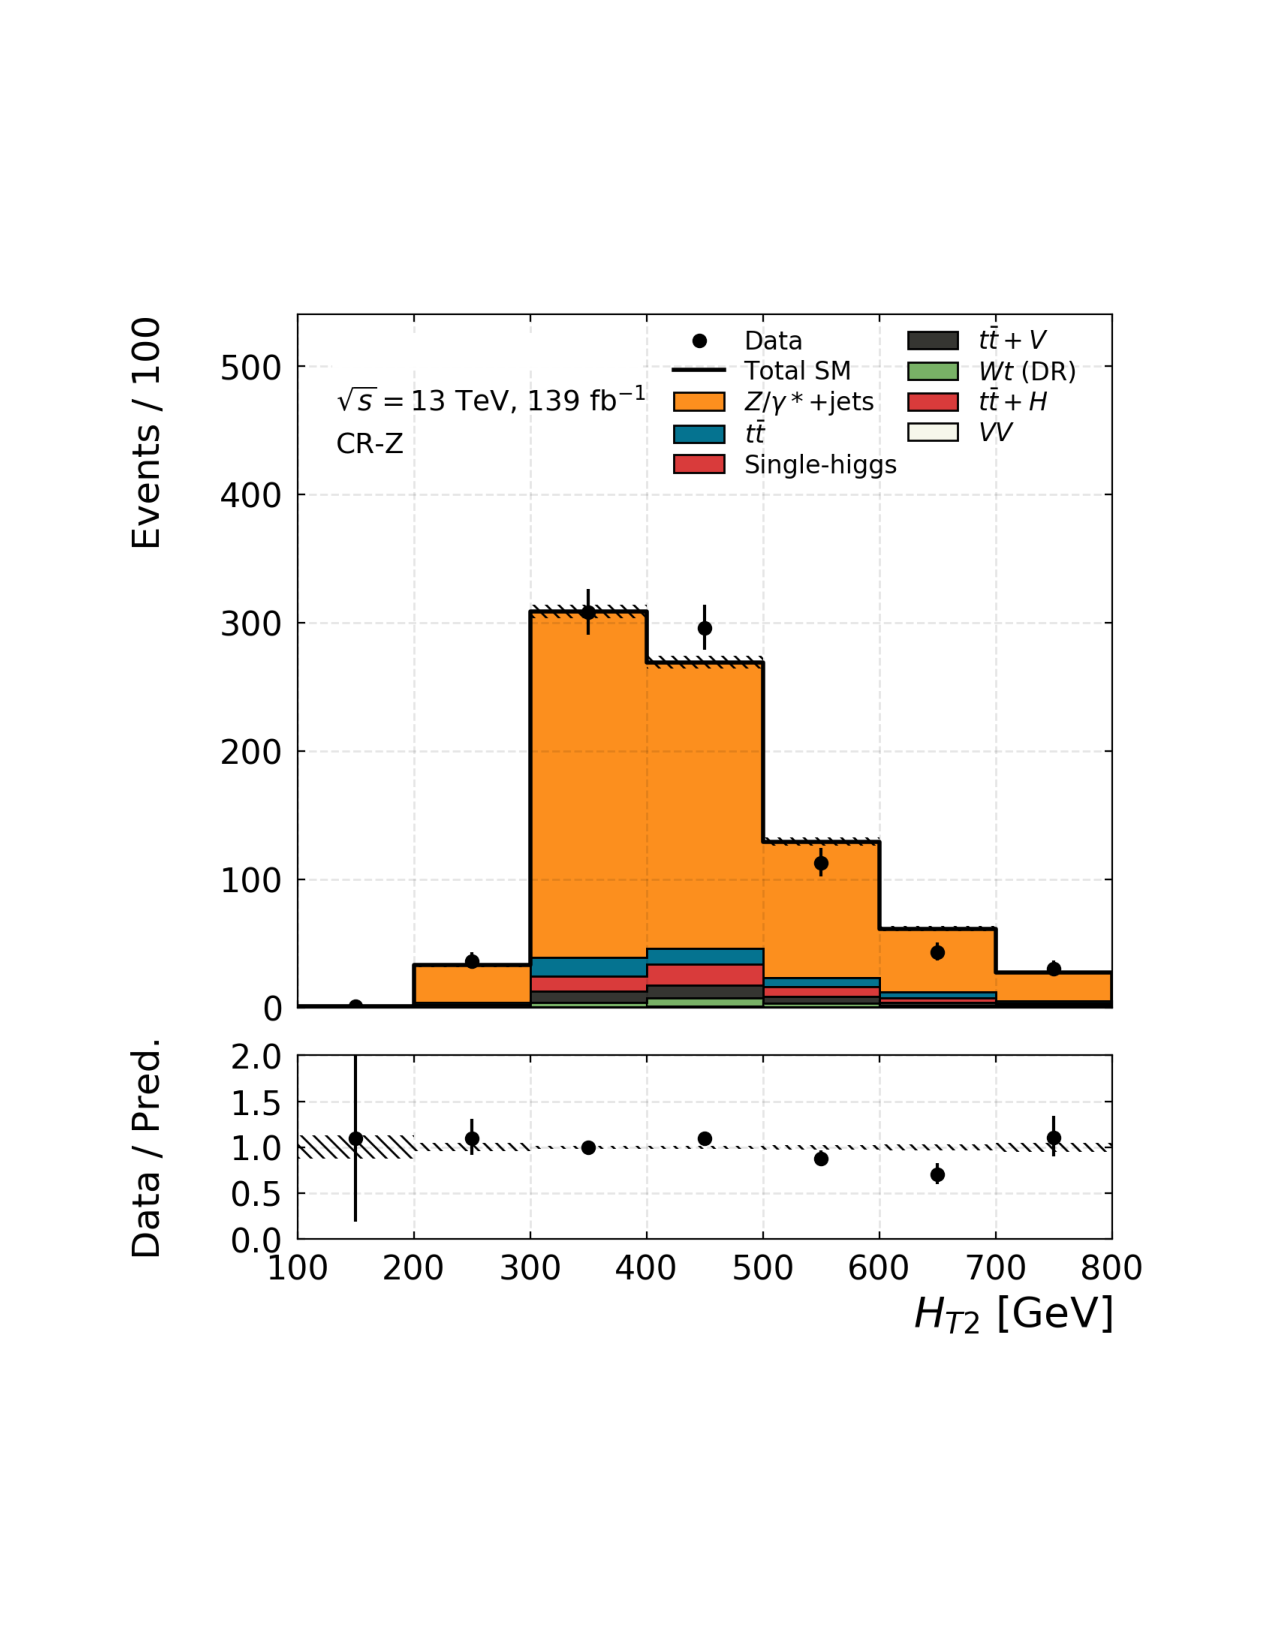
\includegraphics[width=0.4\textwidth]{figures/search_hh/bkg_estimate/crvr/crzhf/crztest_HT2}
    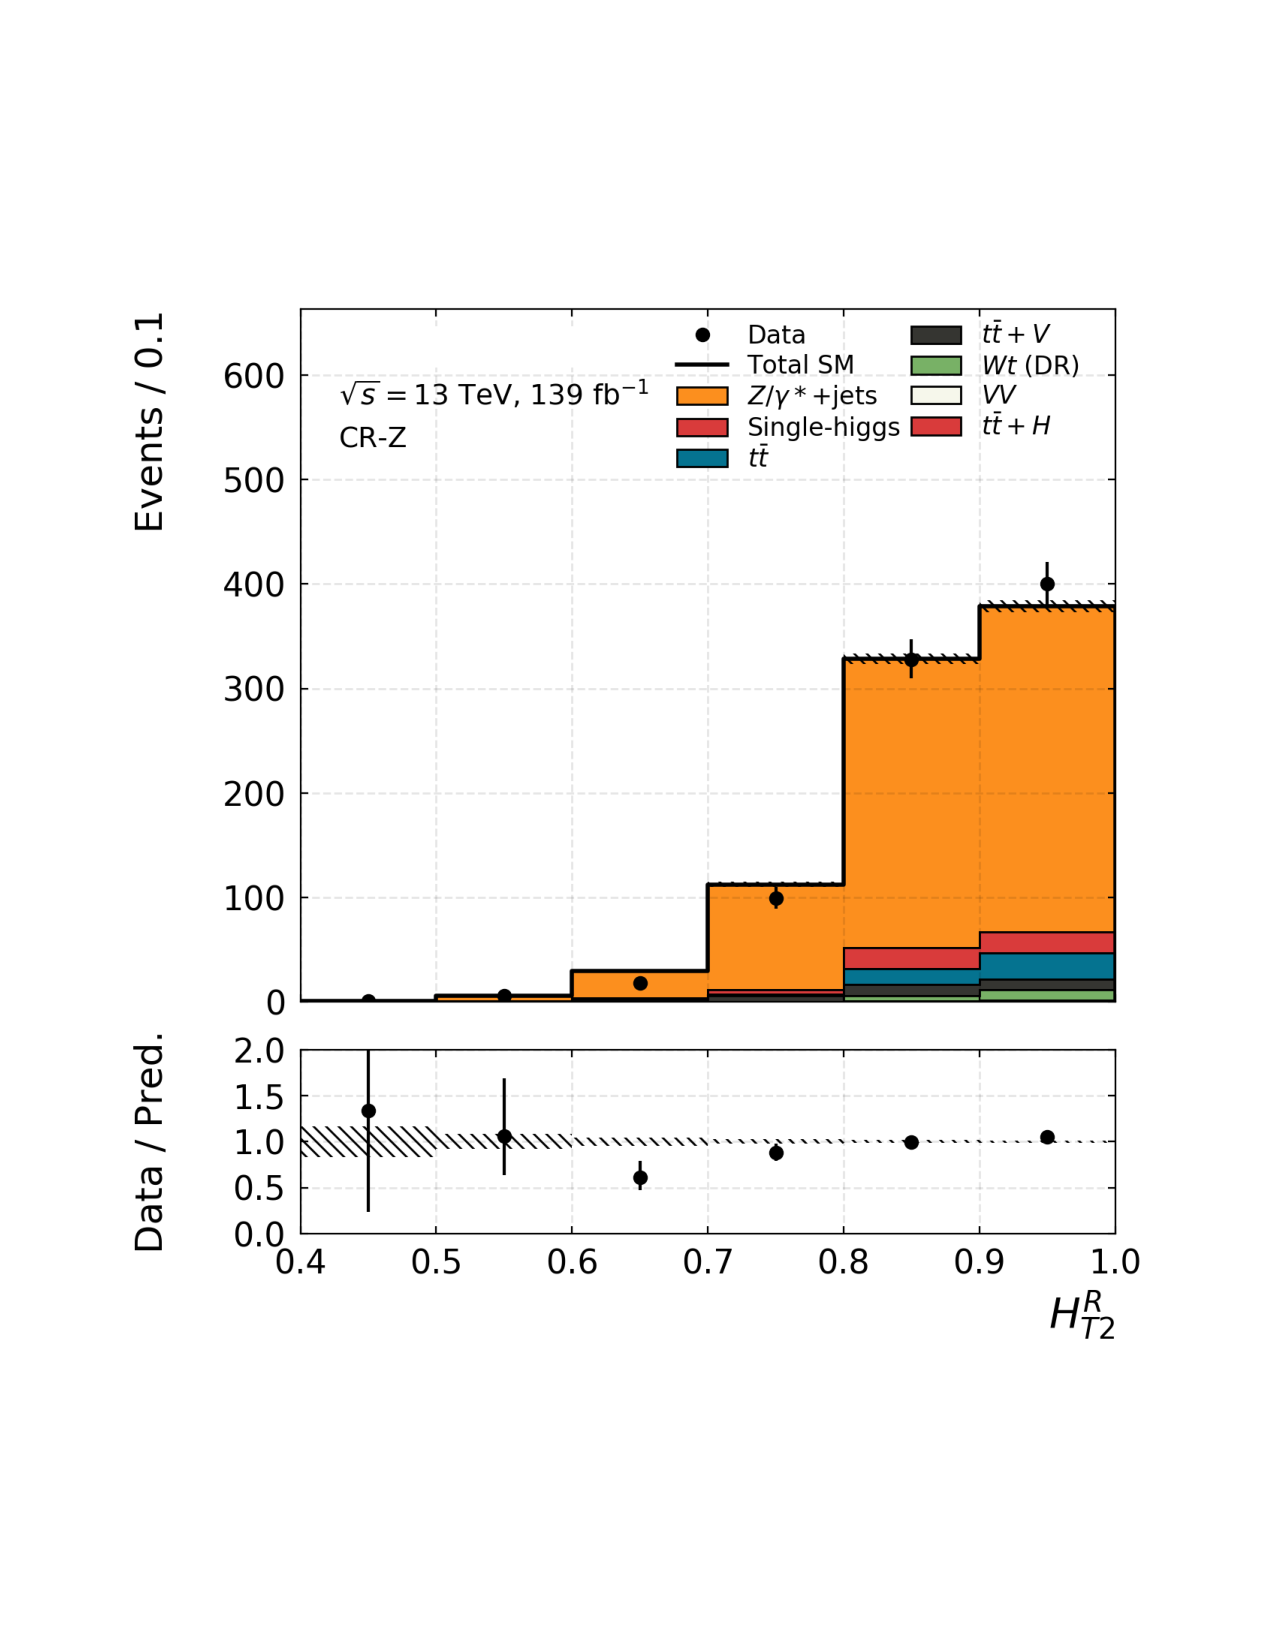
\includegraphics[width=0.4\textwidth]{figures/search_hh/bkg_estimate/crvr/crzhf/crztest_HT2Ratio}
    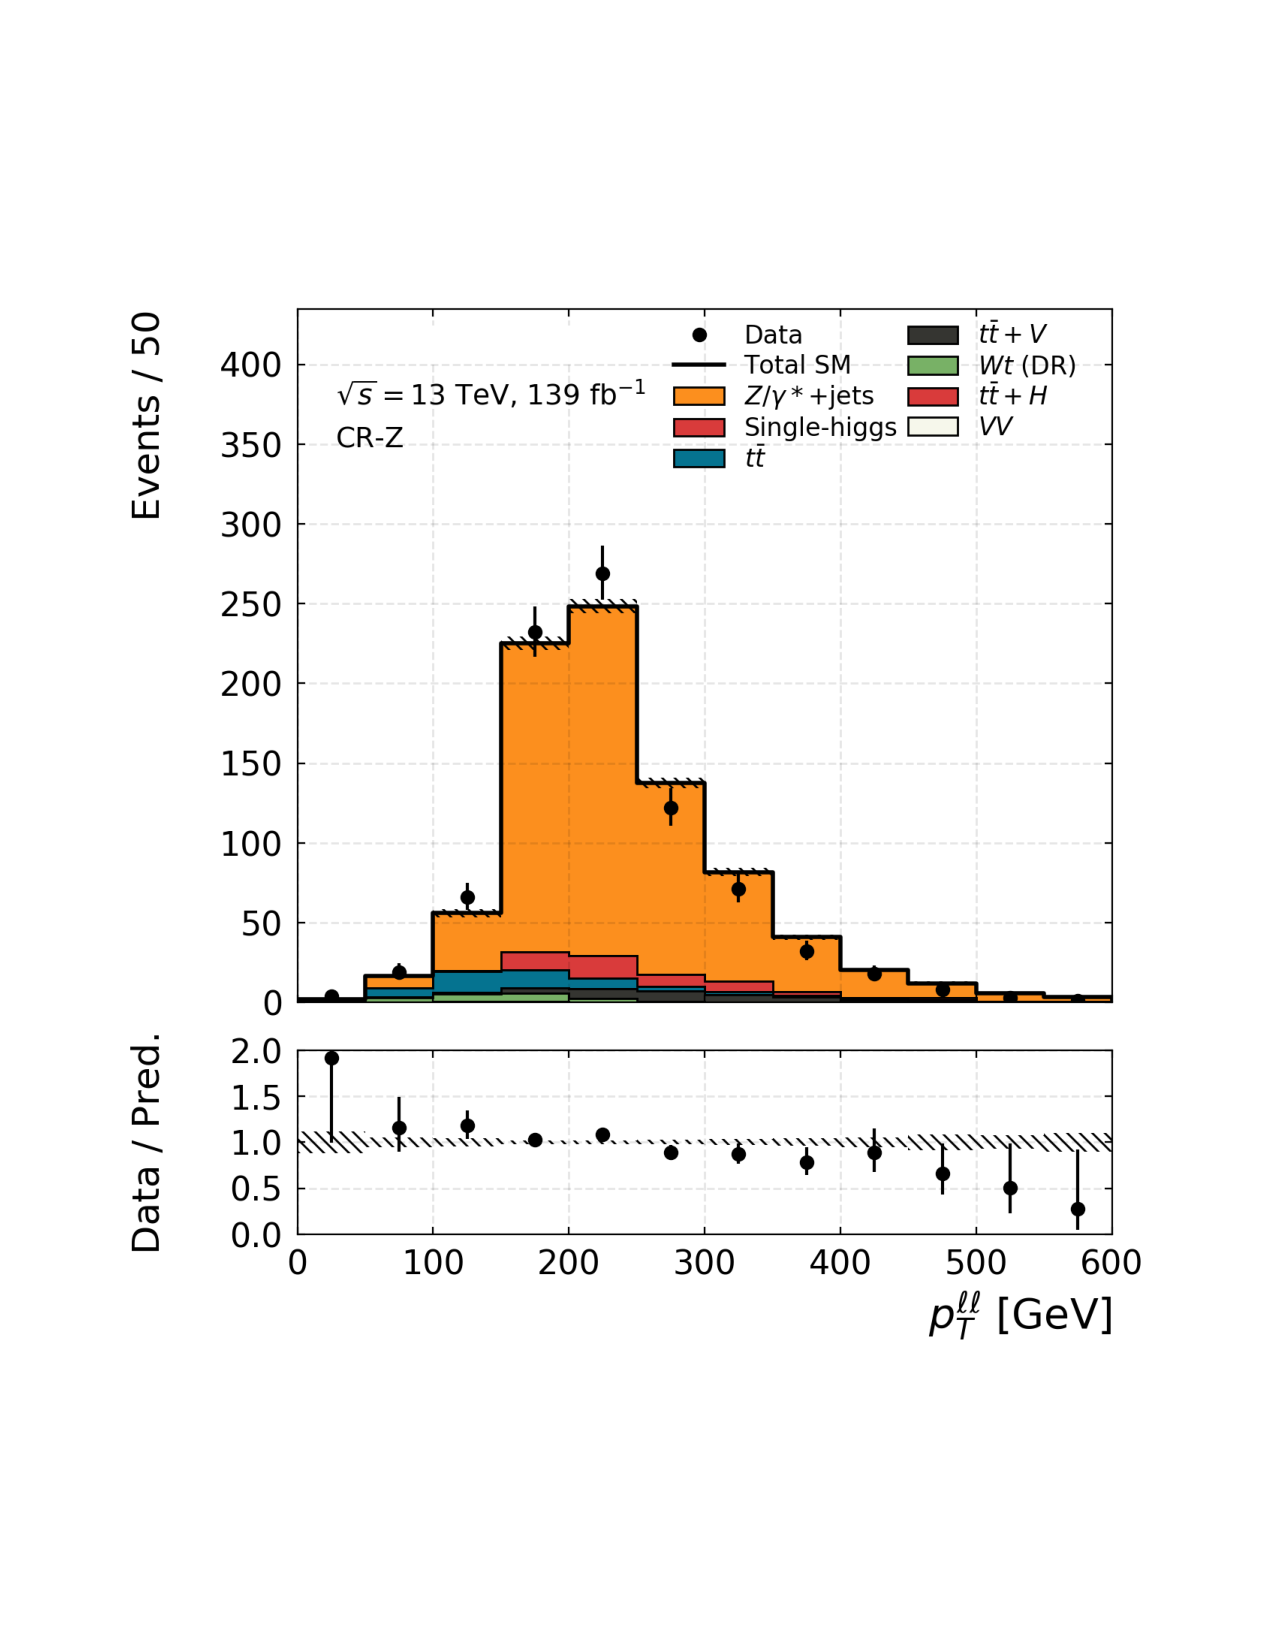
\includegraphics[width=0.4\textwidth]{figures/search_hh/bkg_estimate/crvr/crzhf/crztest_pTll}
    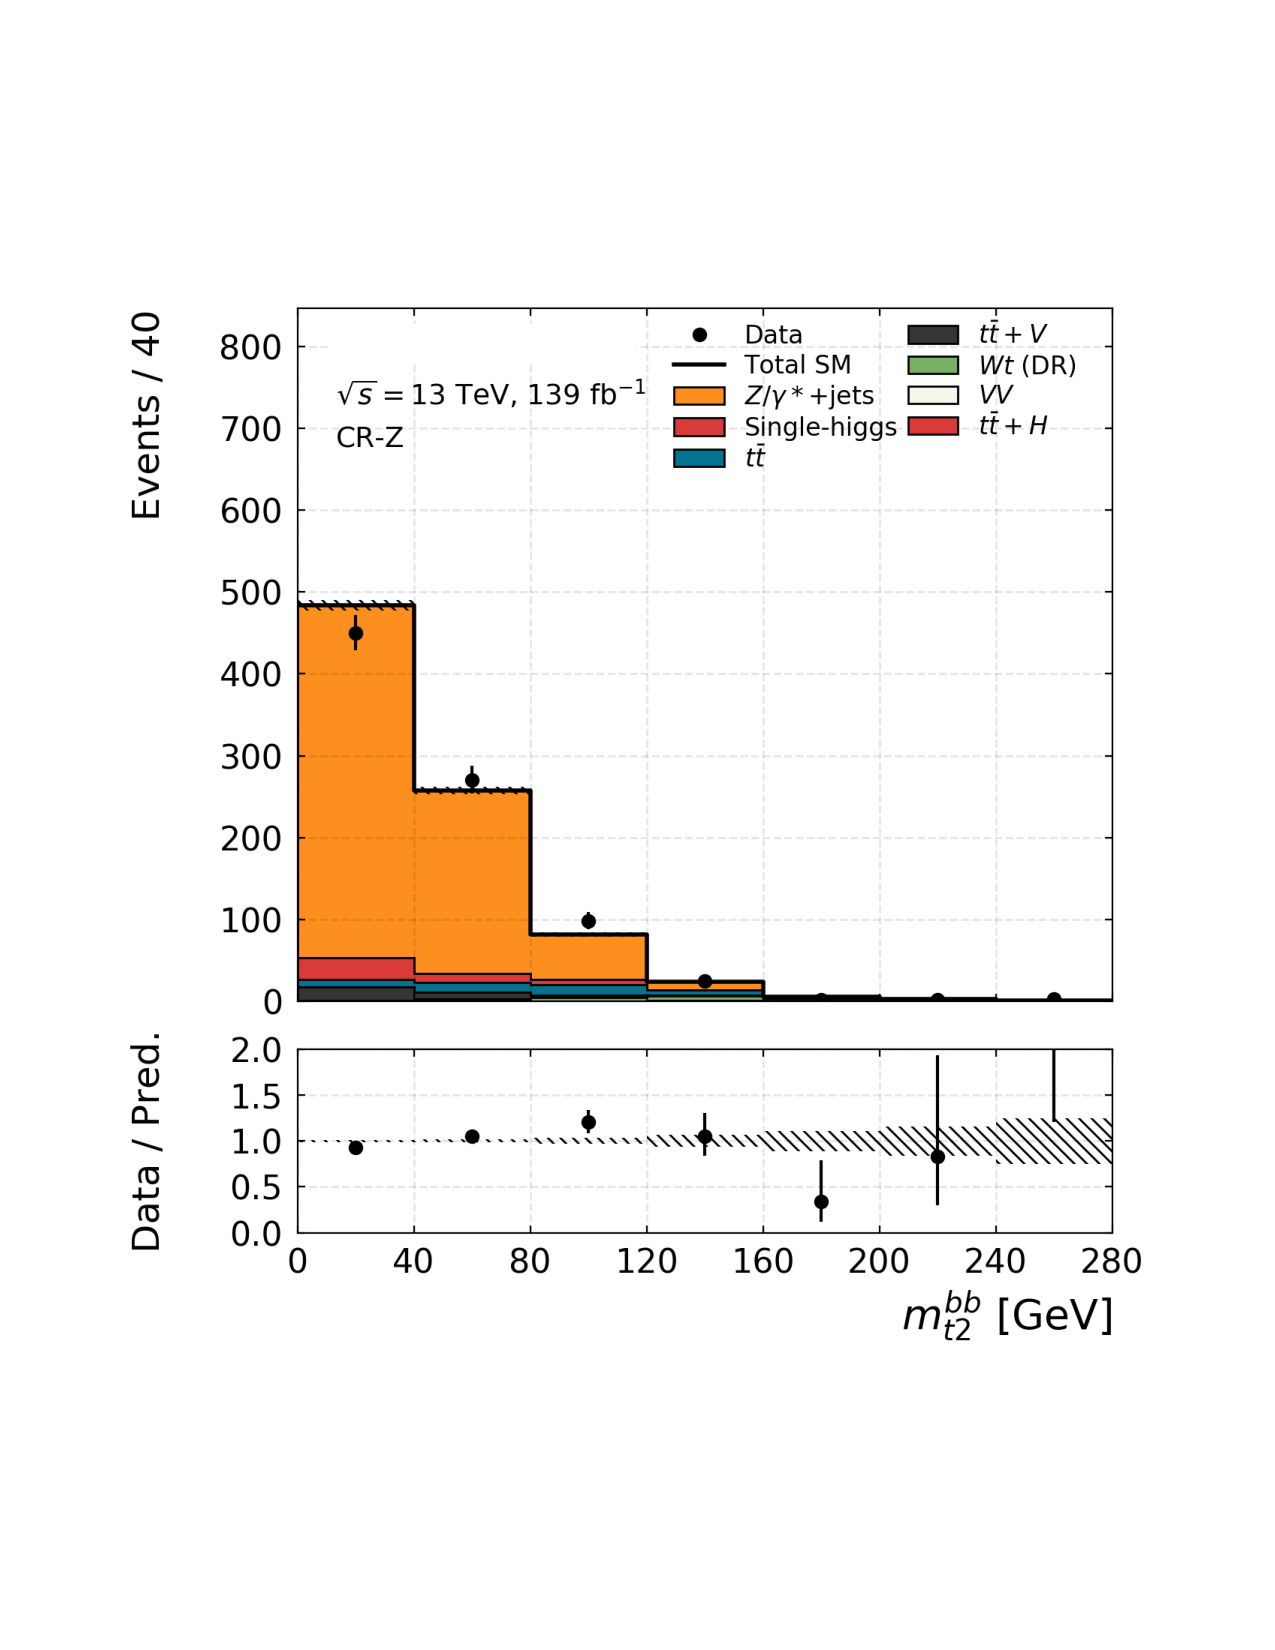
\includegraphics[width=0.4\textwidth]{figures/search_hh/bkg_estimate/crvr/crzhf/crztest_mt2_bb}
    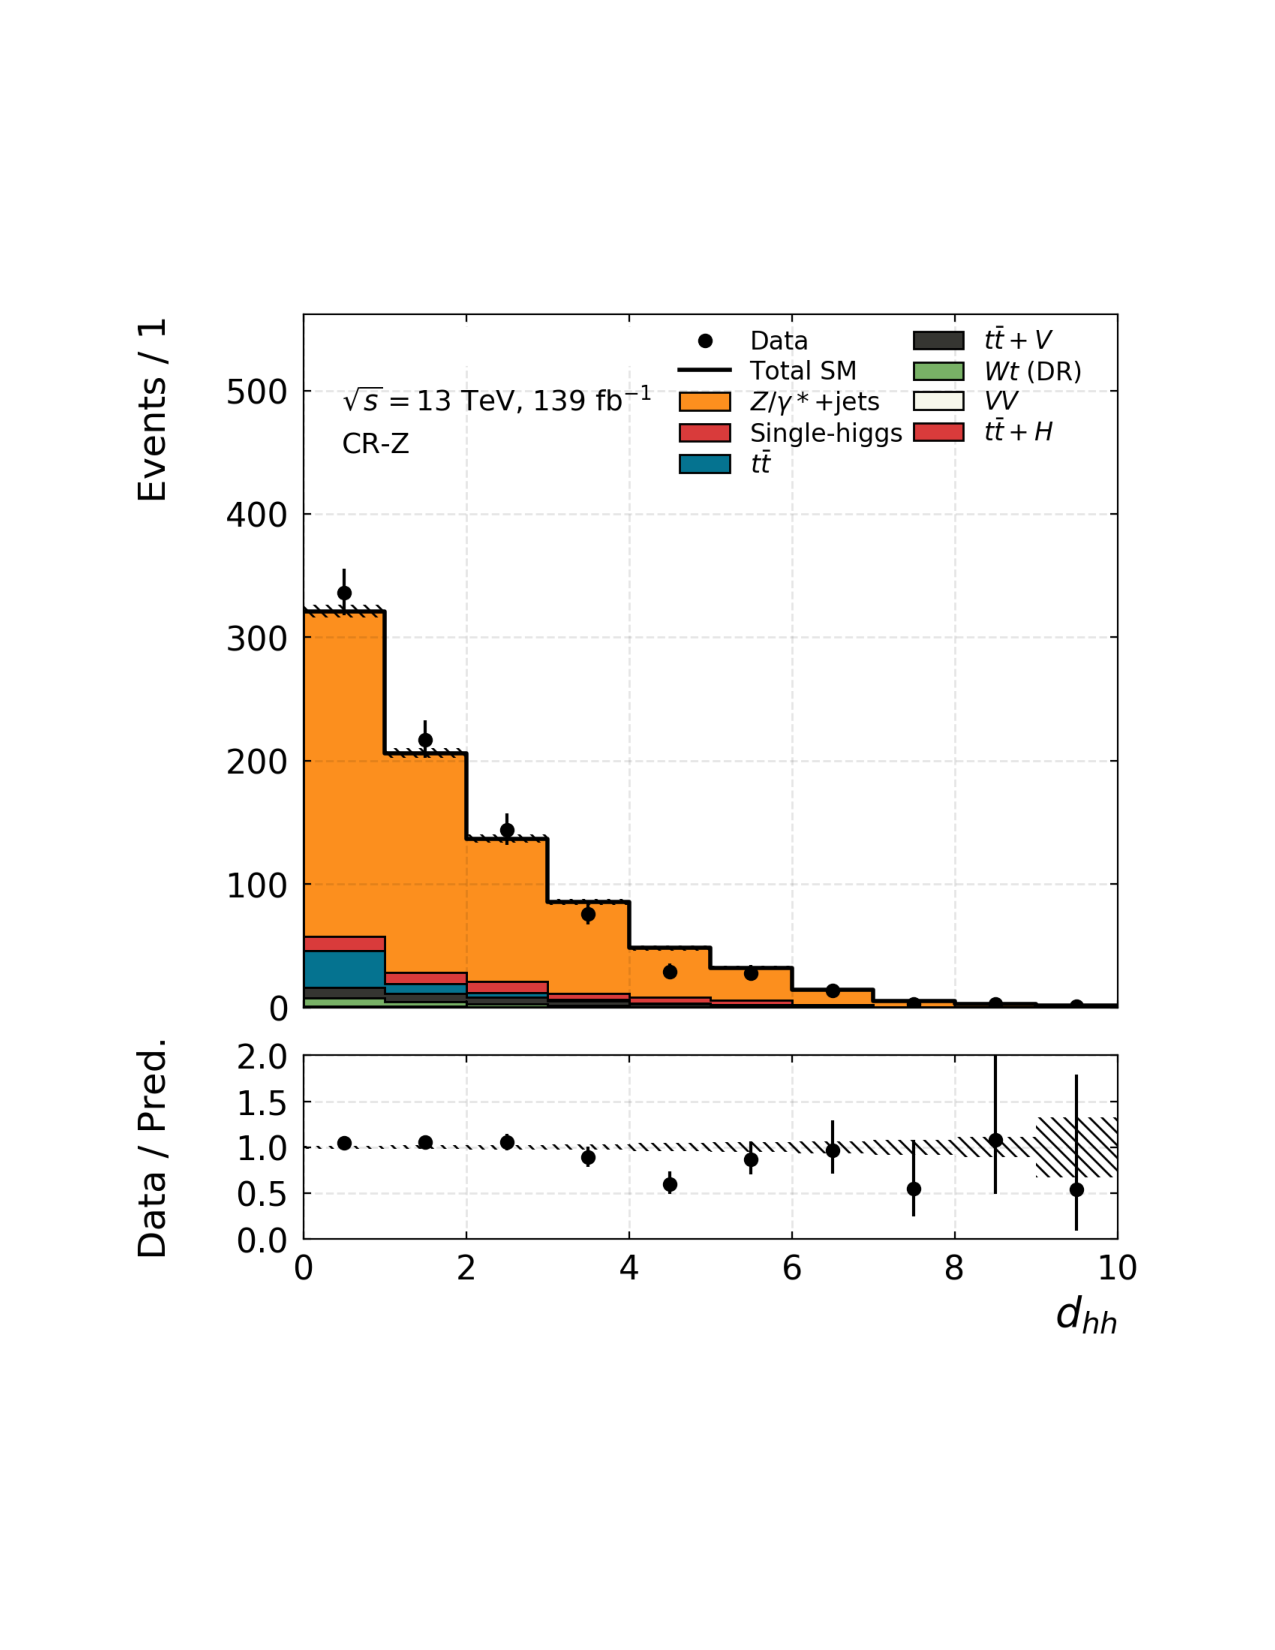
\includegraphics[width=0.4\textwidth]{figures/search_hh/bkg_estimate/crvr/crzhf/crztest_NN_d_hh}
    \caption{
    Kinematic distributions in the $Z$+heavy flavor control region, CR-Z+HF.
    The error bands include only the statistical uncertainty.
    The normalization factors obtained from the background-only fit (Table \ref{tab:hh_norm_factors}) are applied
    to the Top (\ttbar~and $Wt$) and $Z$+jets MC processes.
    }
    \label{fig:crz_kin_plots_2}
\end{figure}
\begin{figure}[!htb]
    \centering
    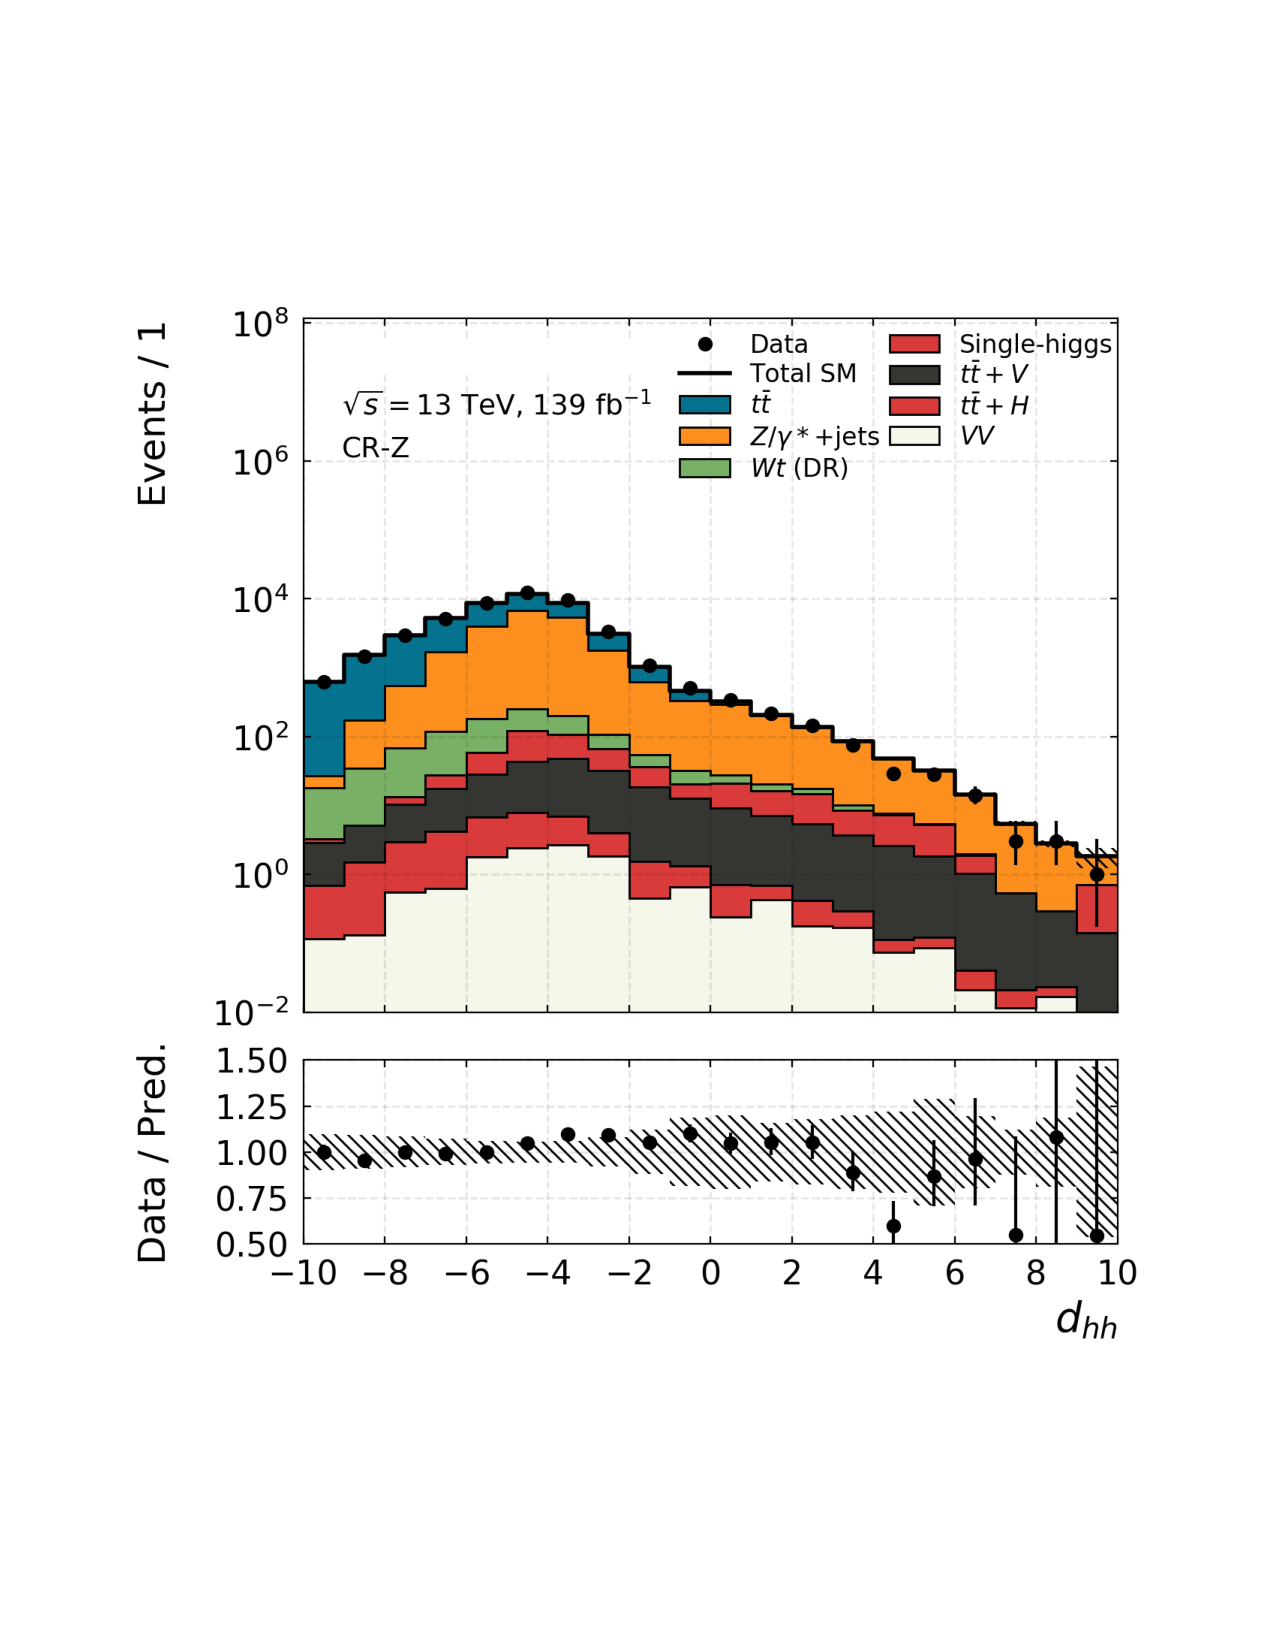
\includegraphics[width=0.65\textwidth]{figures/search_hh/bkg_estimate/crvr/crzhf/crztest_NN_d_hh_fullsys}
    \caption{
    $d_{hh}$ distribution in the $Z$+HF CR without the $d_{hh}$ selection of the $Z$+HF CR applied.
    The error band in the ratio include both statistical and systematic uncertainties while the
    error band in the histogram includes statistical uncertainty only.
    The normalization factors obtained from the background-only fit (Table \ref{tab:hh_norm_factors}) are applied
    to the Top (\ttbar~and $Wt$) and $Z$+jets MC processes.
    }
    \label{fig:crz_nm1_dhh}
\end{figure}

%%%%%%%%%%%%%%%%%%%%%%%%%%%%%%%%%%%%%%%%%%%%%%%%%%%%%%%%%%%%%%%%%%%%%%%%%%%%%%%%%%%
%%%%%%%%%%%%%%%%%%%%%%%%%%%%%%%%%%%%%%%%%%%%%%%%%%%%%%%%%%%%%%%%%%%%%%%%%%%%%%%%%%%
%%%%%%%%%%%%%%%%%%%%%%%%%%%%%%%%%%%%%%%%%%%%%%%%%%%%%%%%%%%%%%%%%%%%%%%%%%%%%%%%%%%
%
% Fakes
%
%%%%%%%%%%%%%%%%%%%%%%%%%%%%%%%%%%%%%%%%%%%%%%%%%%%%%%%%%%%%%%%%%%%%%%%%%%%%%%%%%%%
%%%%%%%%%%%%%%%%%%%%%%%%%%%%%%%%%%%%%%%%%%%%%%%%%%%%%%%%%%%%%%%%%%%%%%%%%%%%%%%%%%%
%%%%%%%%%%%%%%%%%%%%%%%%%%%%%%%%%%%%%%%%%%%%%%%%%%%%%%%%%%%%%%%%%%%%%%%%%%%%%%%%%%%

\FloatBarrier
\subsection{Sources of Fake and Non-Prompt Leptons}
\label{sec:hh_fakes}

In this section we describe the estimation of sources of fake and non-prompt leptons.
The analysis uses the Same-sign Extrapolation Method, described in detail in Section~\ref{sec:fakes}.
In order to perform the estimate of fake leptons in this manner, we define a set of fake lepton control
regions which are defined similarly as the analysis CRs and SRs, but with the opposite-sign (OS)
lepton requirement inverted, instead requiring same-sign (SS) lepton pairs.
This is as described in Section~\ref{sec:fakes}.
On top of this, for the present analysis, we further invert the analysis' \dhh requirements in the SS
regions.
This is done so that we may increase the SS sample statistics further than if we were to rely solely
on using the SS sample with all other selections remaining the same as their OS counterparts.
In this way, we extrapolate over the \dhh quantity in addition to the lepton charge requirement
and Equation~\ref{eq:ss_extrap} is modified to include the factor $\varepsilon^{\dhh}$, as indicated in Equation~\ref{eq:ss_extrap_dhh}.

\begin{align}
    N_{\text{OS}}^{\text{fake}} &= \varepsilon^{\dhh} \times f^{SS \rightarrow OS} \times N_{\text{SS}}^{\text{fake}} \nonumber \\
        &= \frac{N_{\text{MC,dhh+}}^{\text{non-prompt}}}{N_{\text{MC,dhh-}}^{\text{non-prompt}}} \times  \frac{ N_{\text{MC,OS}}^{\text{fake}} }{ N_{\text{MC,SS}}^{\text{fake}} } \times ( N_{\text{data,SS}} - N_{\text{MC,SS}}^{\text{real}} ),
        \label{eq:ss_extrap_dhh}
\end{align}
where $N_{\text{MC,dhh+}}$ ($N_{\text{MC,dhh-}}$) gives the numbers of events in the non-inverted (inverted)
\dhh selections.
Additional systematic uncertainties related to the measurement of the $\varepsilon^{\dhh}$ quantity are
assessed on top of those already described in Section~\ref{sec:common_systematics}.

Using truth level information available in the MC, the fake and non-prompt sources of leptons are
categorized either as being due to semi-leptonic decays of heavy-flavor hadrons (resulting in non-prompt electrons
or muons), non-prompt electrons due to photon conversions, or grouped into a catch-all category not
falling under any of the others already defined (`other').

Figures~\ref{fig:fake_val_srdf} and \ref{fig:fake_val_srsf} show the data and MC distributions in the same-sign
selections used for deriving the same-sign extrapolation for the lepton transverse momenta, dilepton invariant
mass, and \dhh observables.
The fake estimate provided entirely by MC is generally able to recover the observation in each region, providing
confidence that the extrapolation factor $f^{SS \rightarrow OS}$, derived using the MC, is correct.

Figure~\ref{fig:fake_val_ss_os_shape} shows the shapes of the data-driven fakes based on the SS data sample
compared to the MC non-prompt estimate in the SS and OS versions of the SR selections.
It is seen that the data-driven fake sample, with the prompt MC events subtracted, has a compatible
shape with the purely MC-based fake estimate for the observable of interest, \dhh.
This provides further support in the extrapolation from the SS to OS events as well as in the extrapolation
over the \dhh observable.

\begin{figure}[!htb]
    \begin{center}
    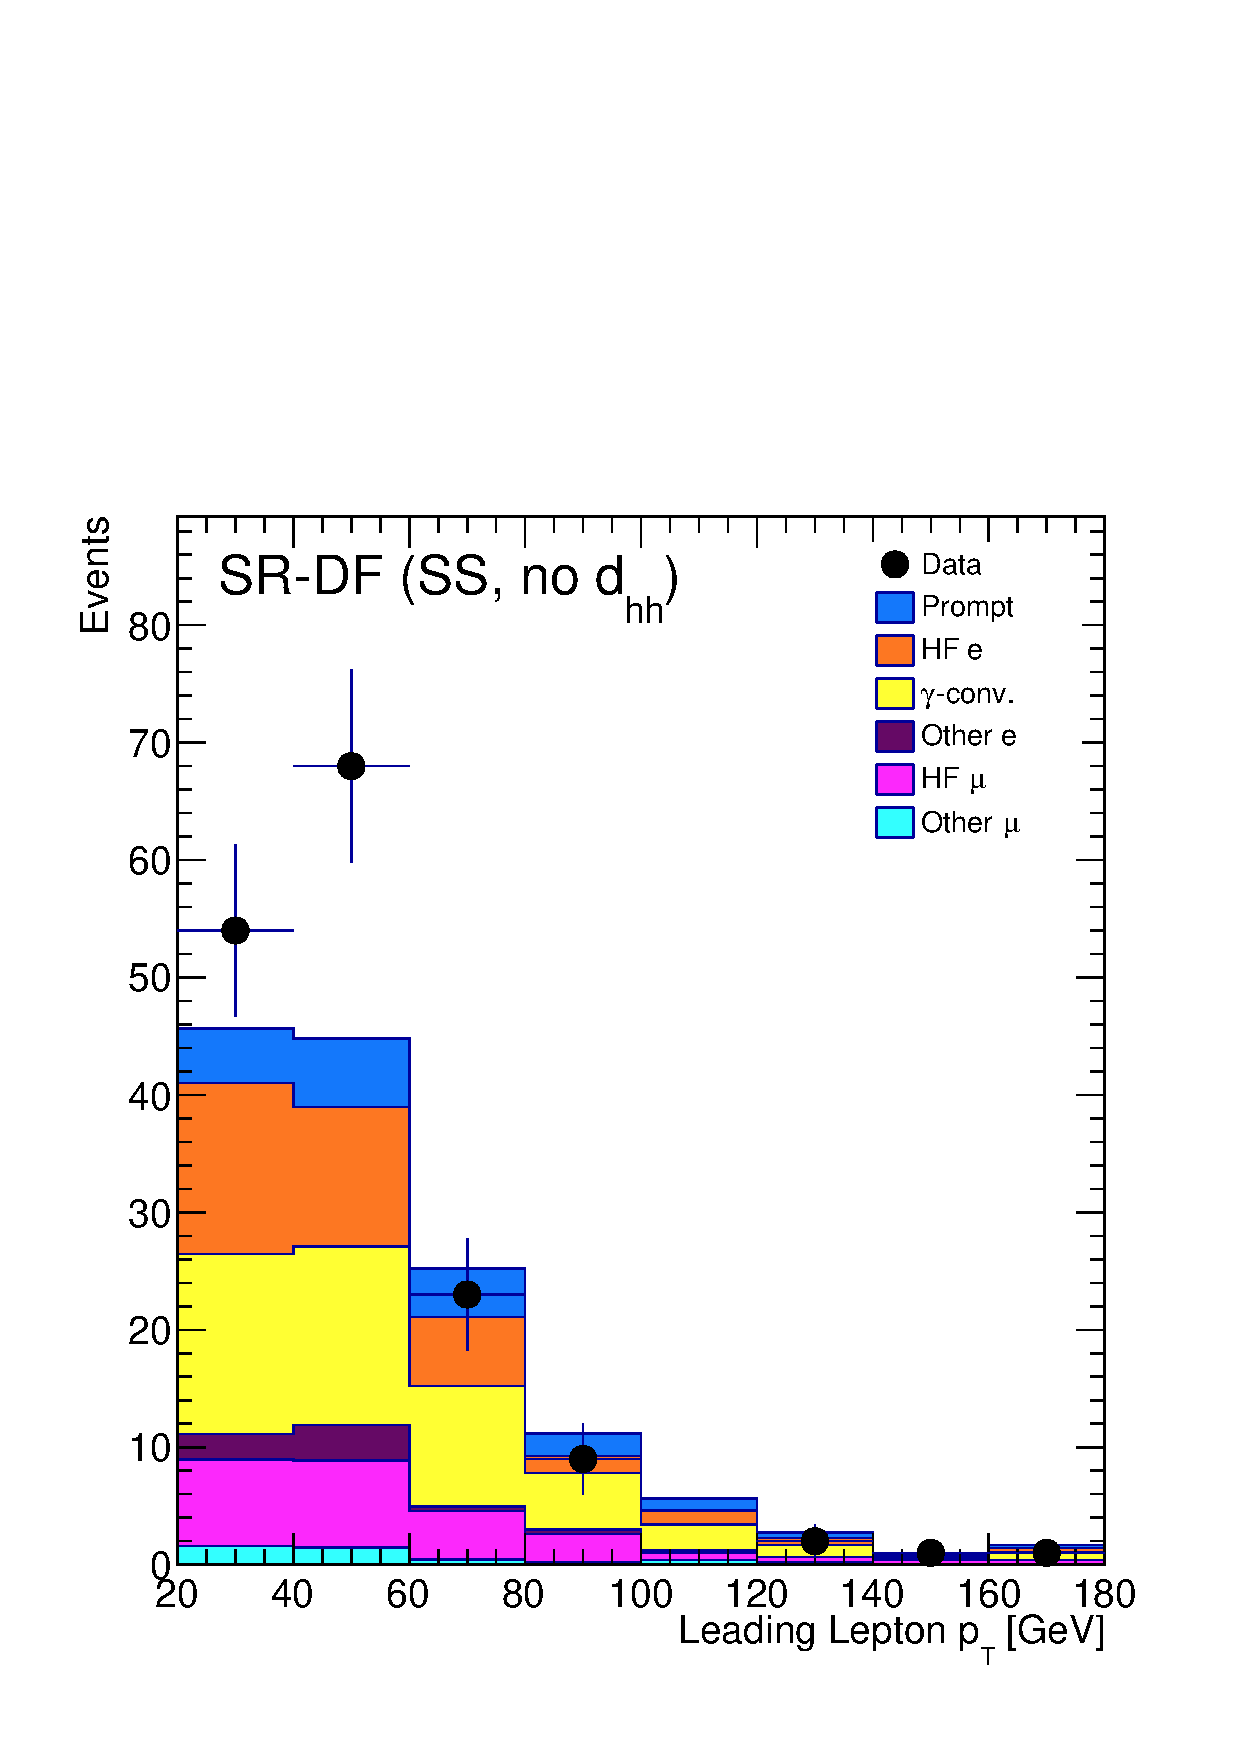
\includegraphics[width=0.45\textwidth]{figures/search_hh/bkg_estimate/fake/fake_val_sr_df_ss_l0_pt}
    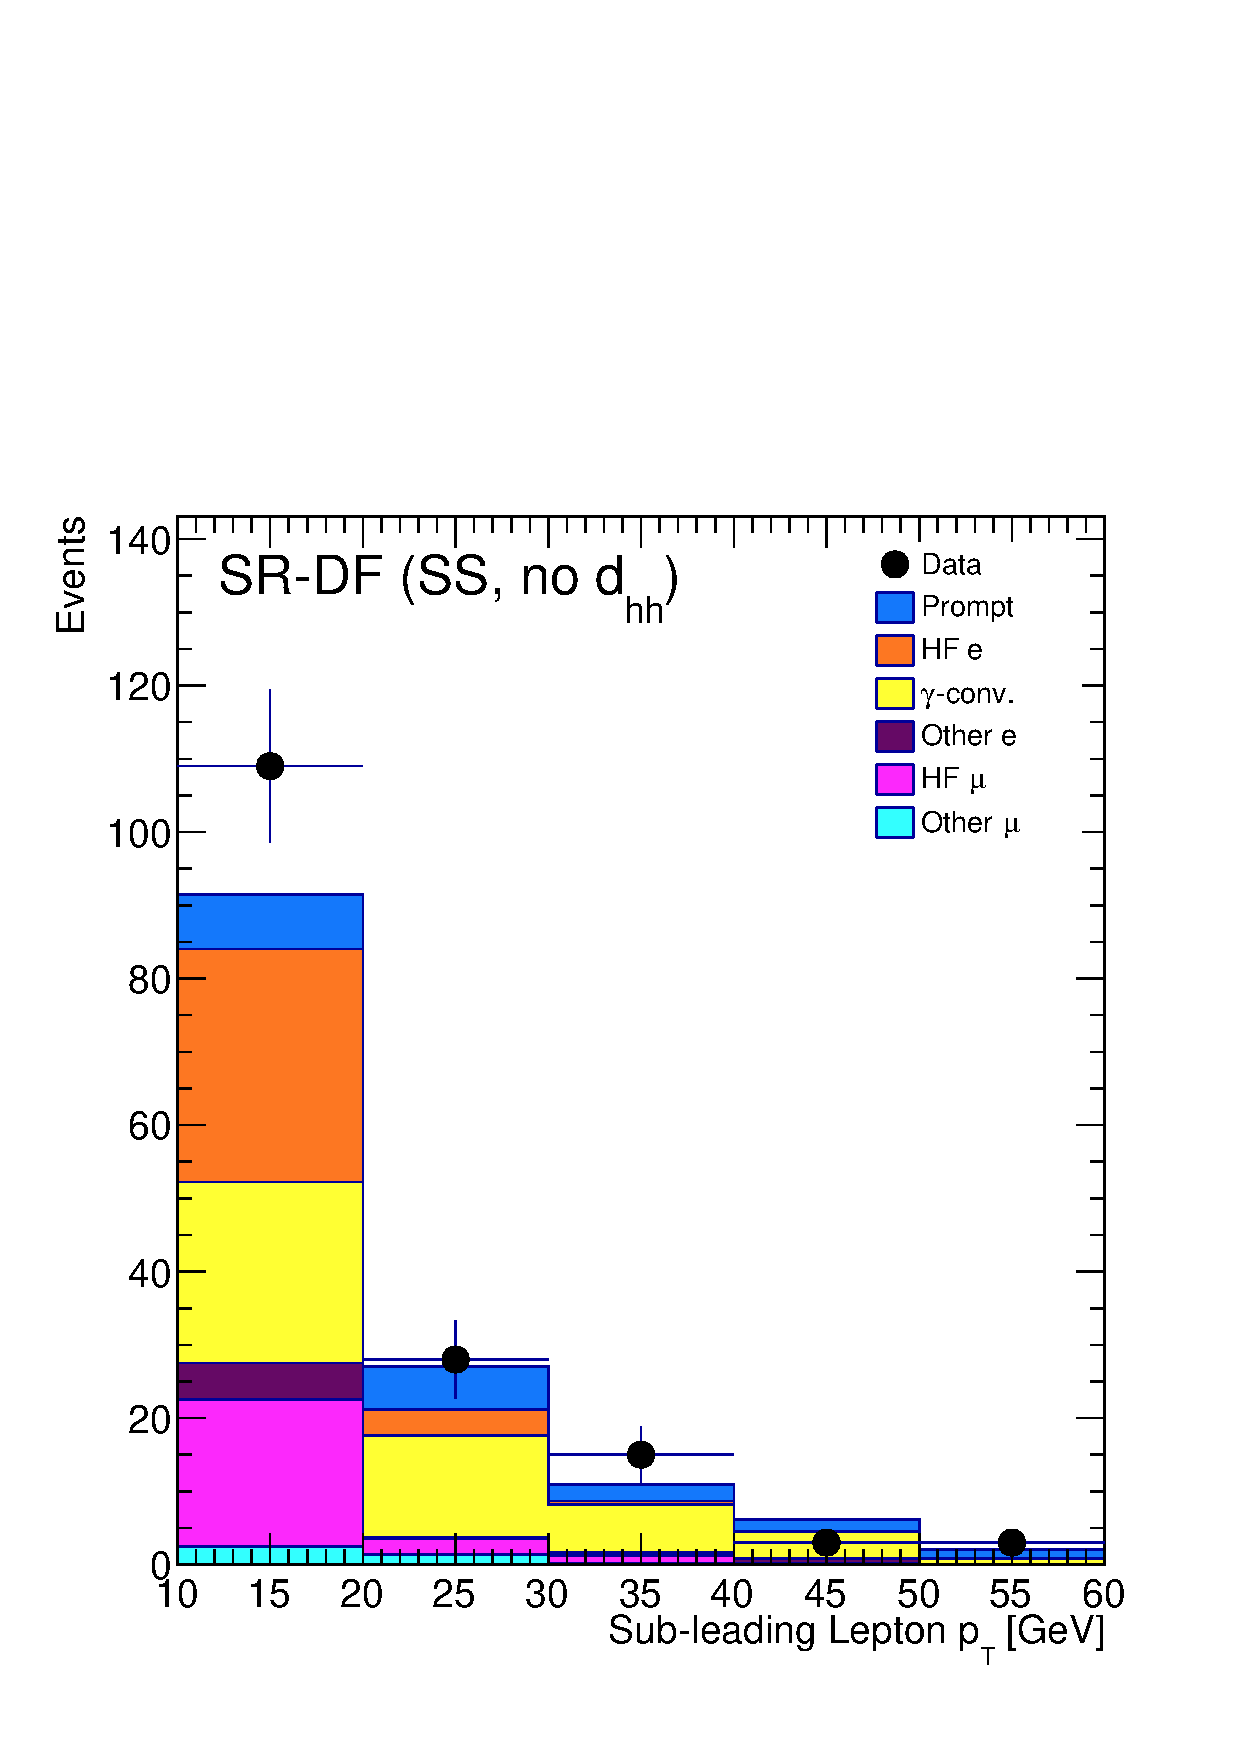
\includegraphics[width=0.45\textwidth]{figures/search_hh/bkg_estimate/fake/fake_val_sr_df_ss_l1_pt}
    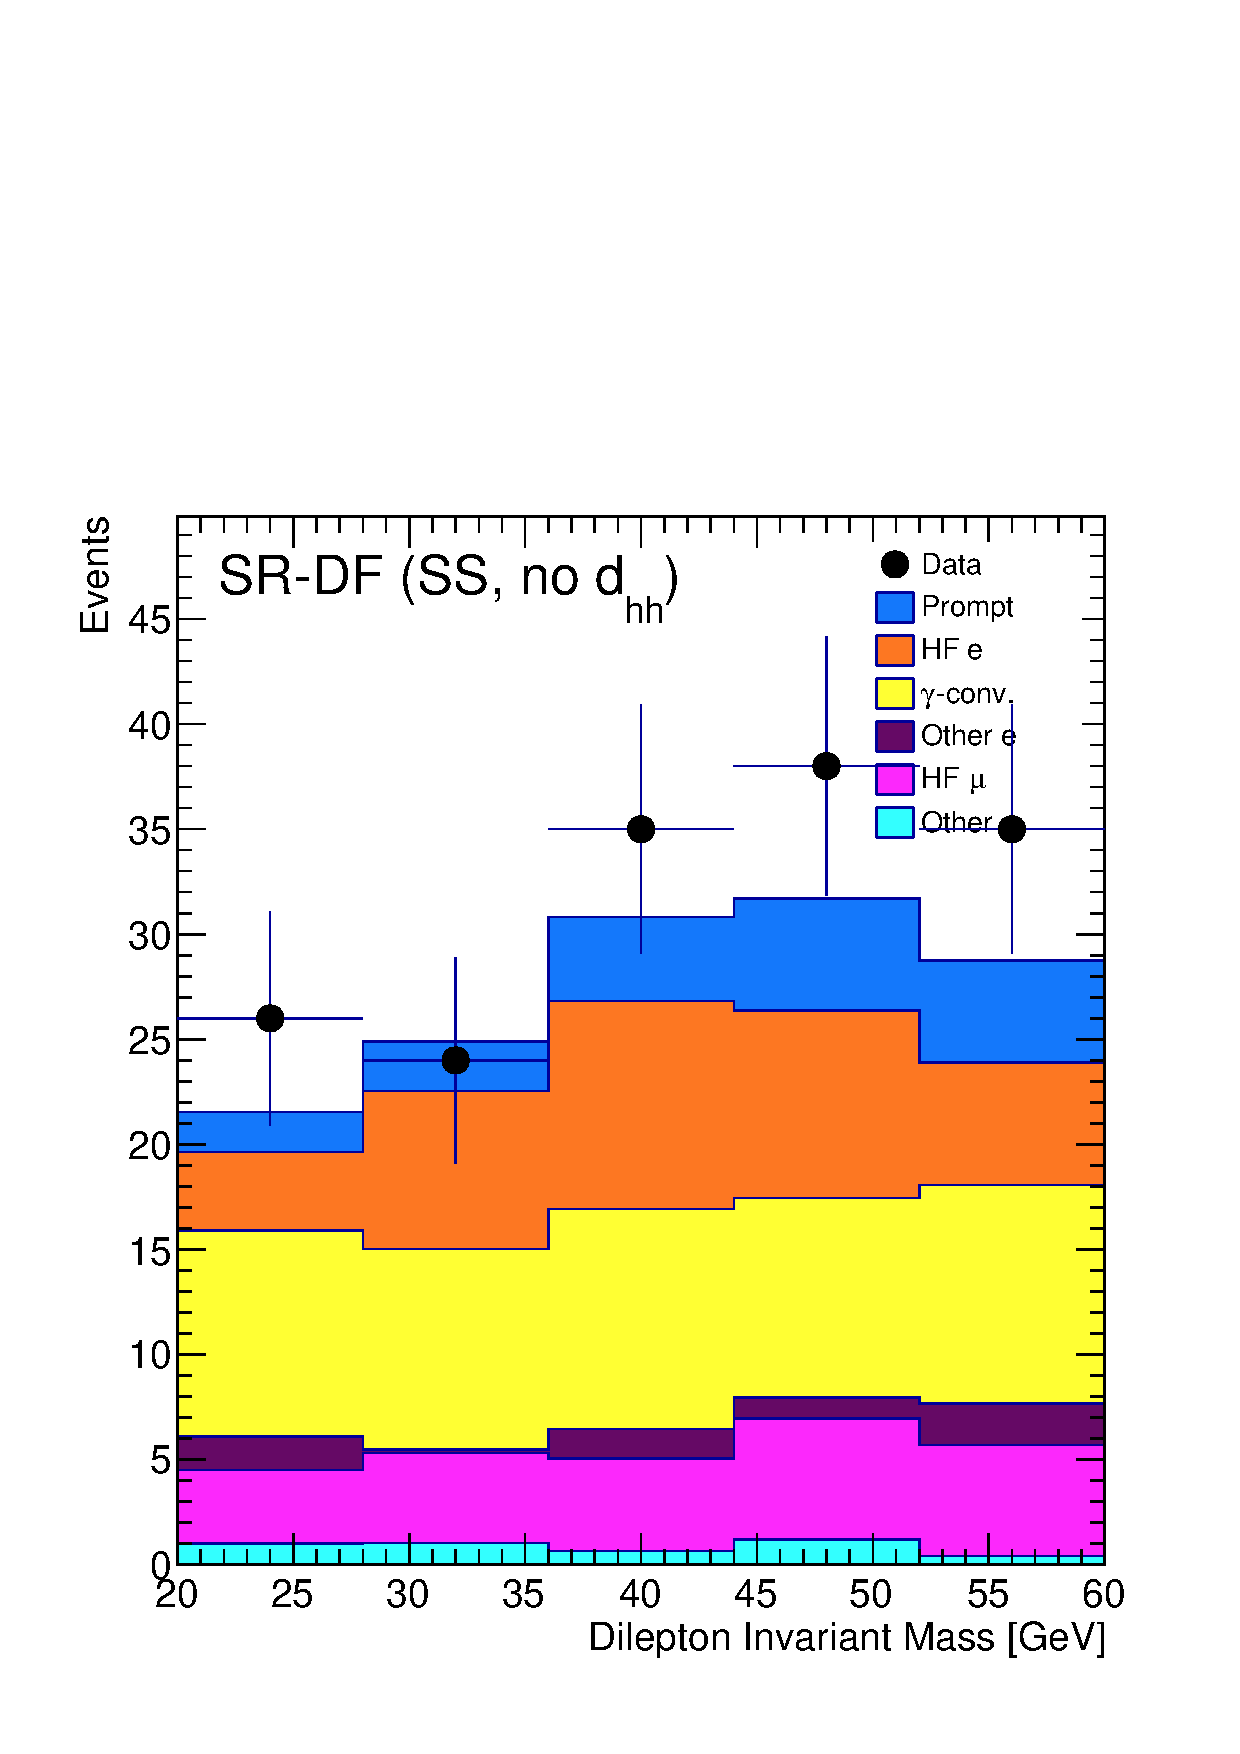
\includegraphics[width=0.45\textwidth]{figures/search_hh/bkg_estimate/fake/fake_val_sr_df_ss_mll}
    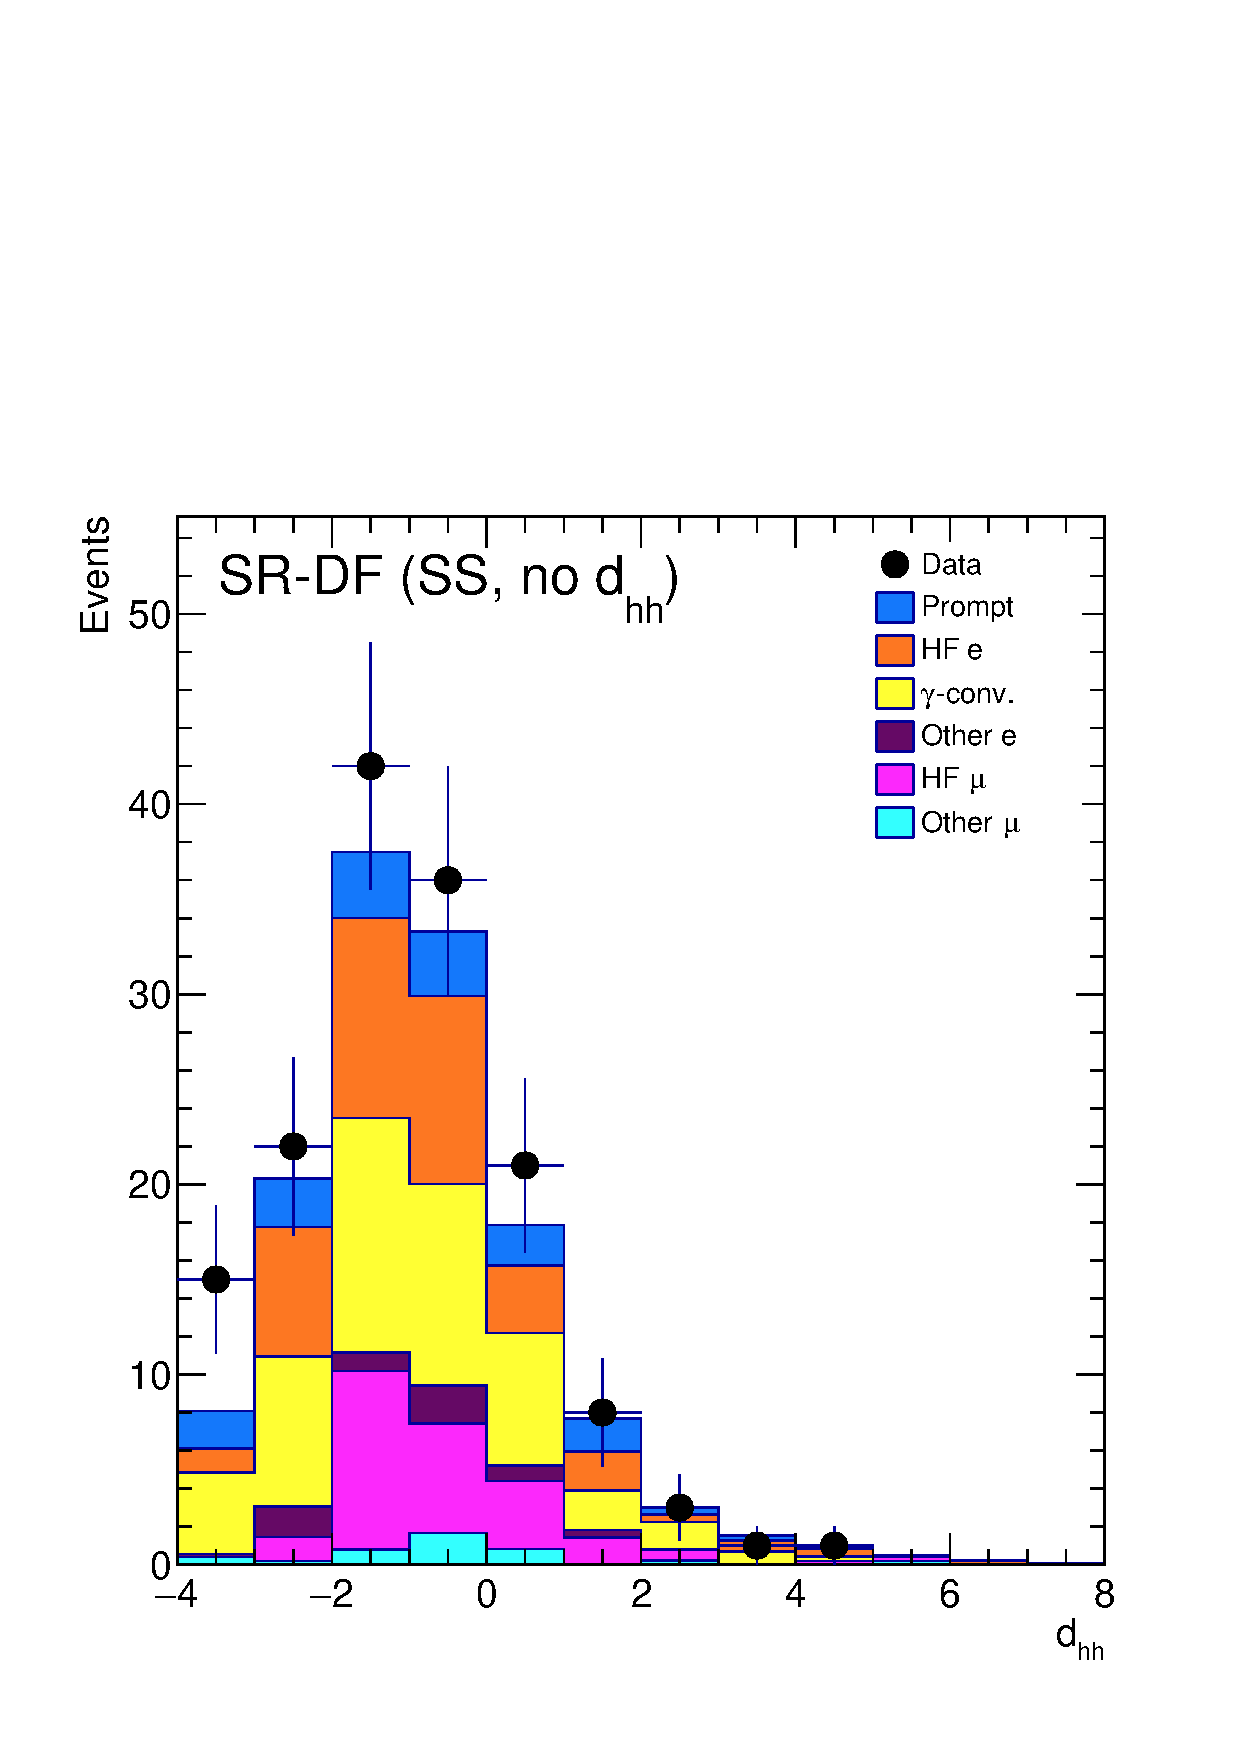
\includegraphics[width=0.45\textwidth]{figures/search_hh/bkg_estimate/fake/fake_val_sr_df_ss_NN_d_hh}
    \caption{
        Data and MC distributions in the same-sign SR-DF selection with the $d_{hh}$ requirement removed.
        The non-prompt MC is broken into the categories described in the text.
        \textbf{\textit{top-left}}: Leading lepton $p_{T}$, \textbf{\textit{top-right}}: Sub-leading lepton $p_{T}$,
        \textbf{\textit{bottom-left}}: dilepton invariant mass, and \textbf{\textit{bottom-right}}: $d_{hh}$.
    }
    \label{fig:fake_val_srdf}
    \end{center}
\end{figure}

\begin{figure}[!htb]
    \begin{center}
    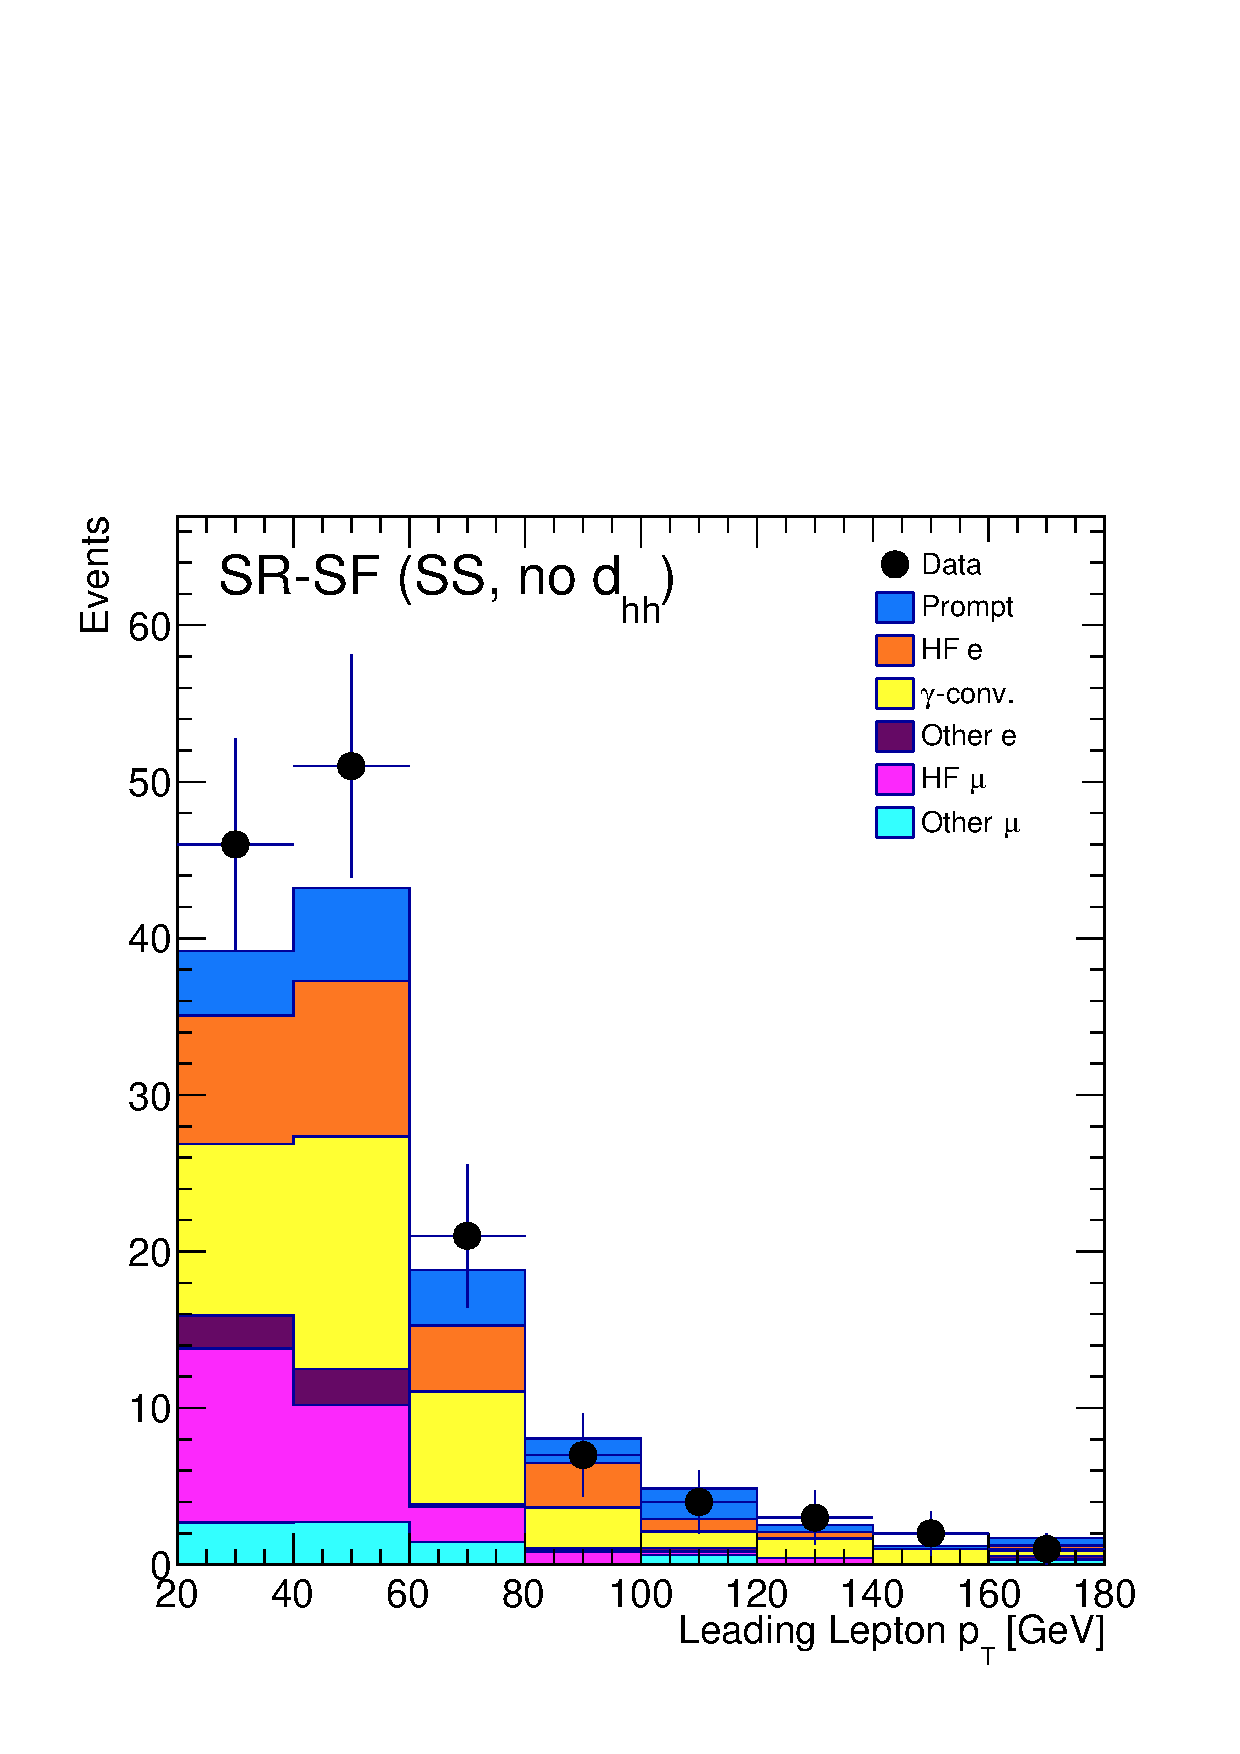
\includegraphics[width=0.45\textwidth]{figures/search_hh/bkg_estimate/fake/fake_val_sr_sf_ss_l0_pt}
    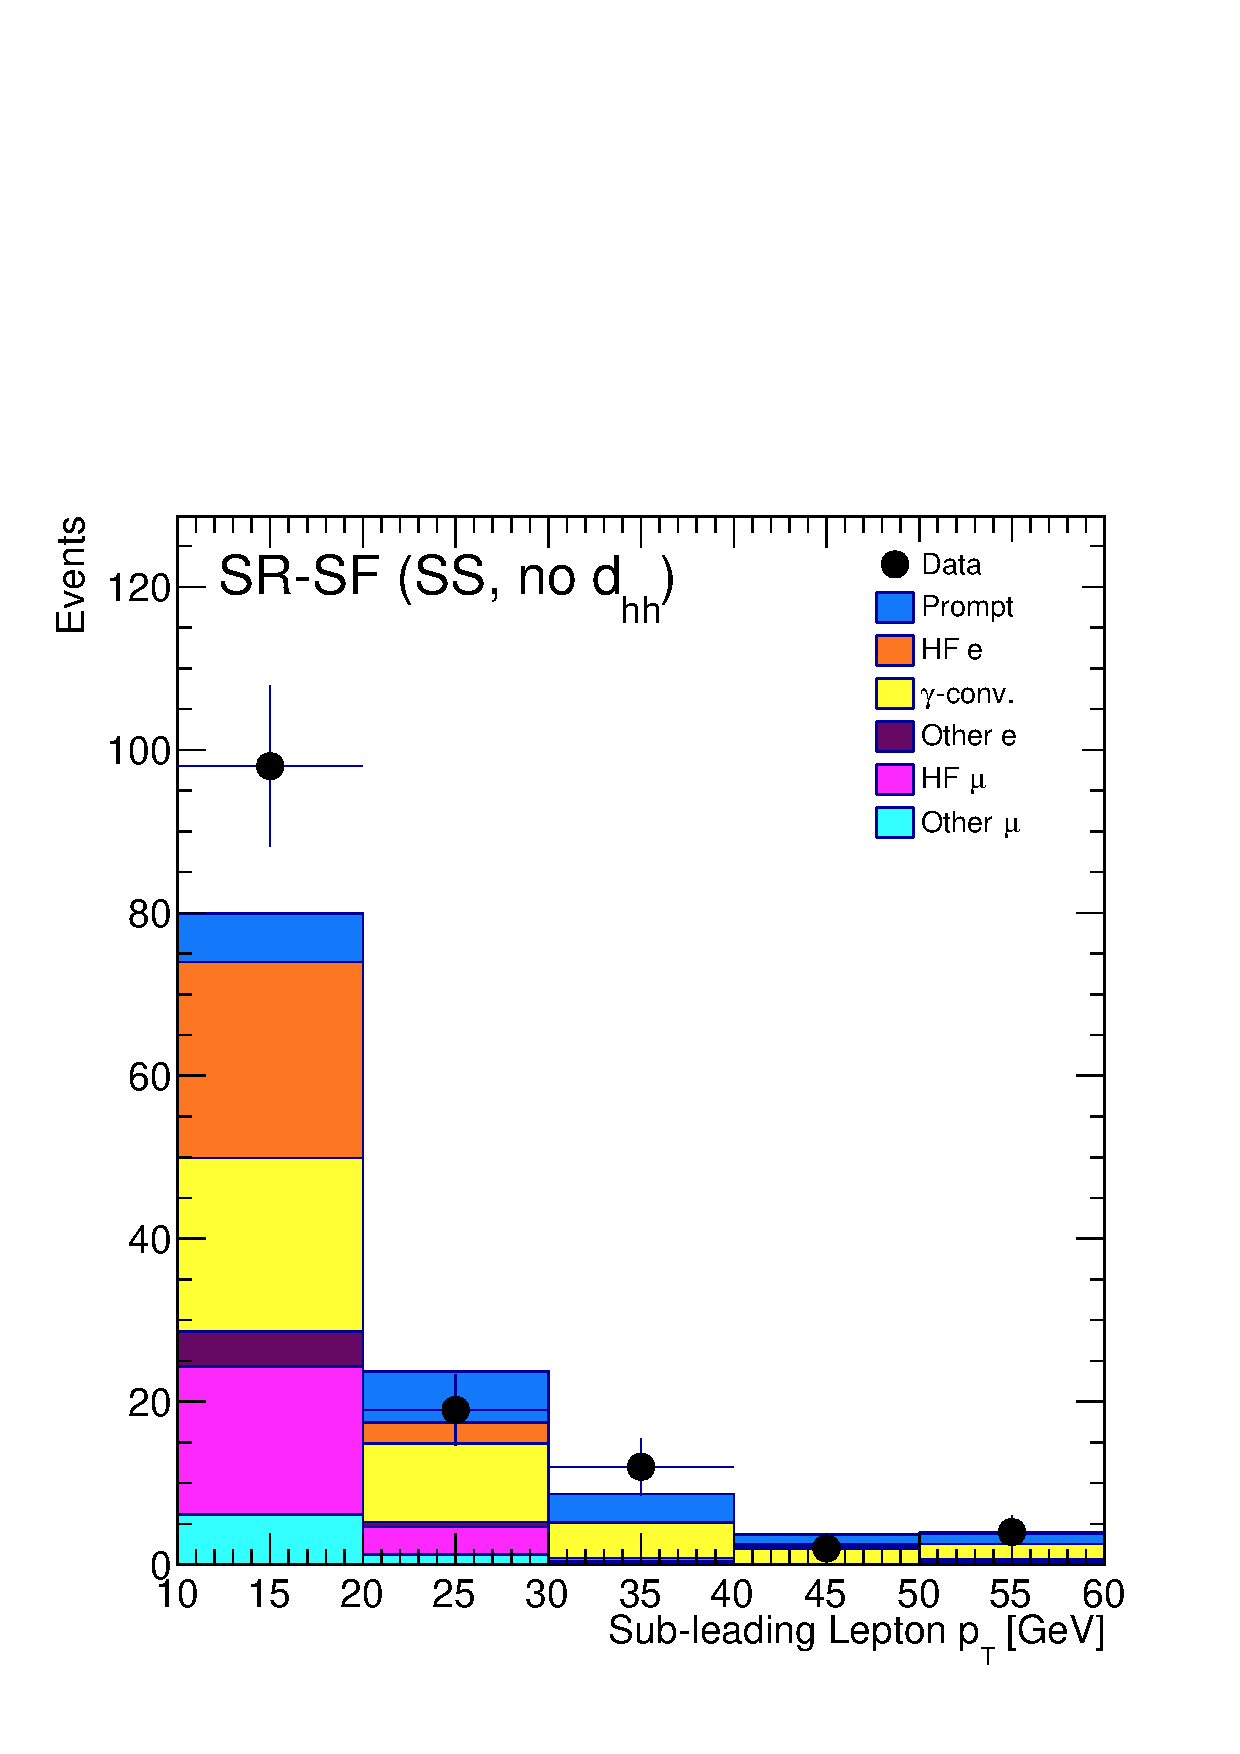
\includegraphics[width=0.45\textwidth]{figures/search_hh/bkg_estimate/fake/fake_val_sr_sf_ss_l1_pt}
    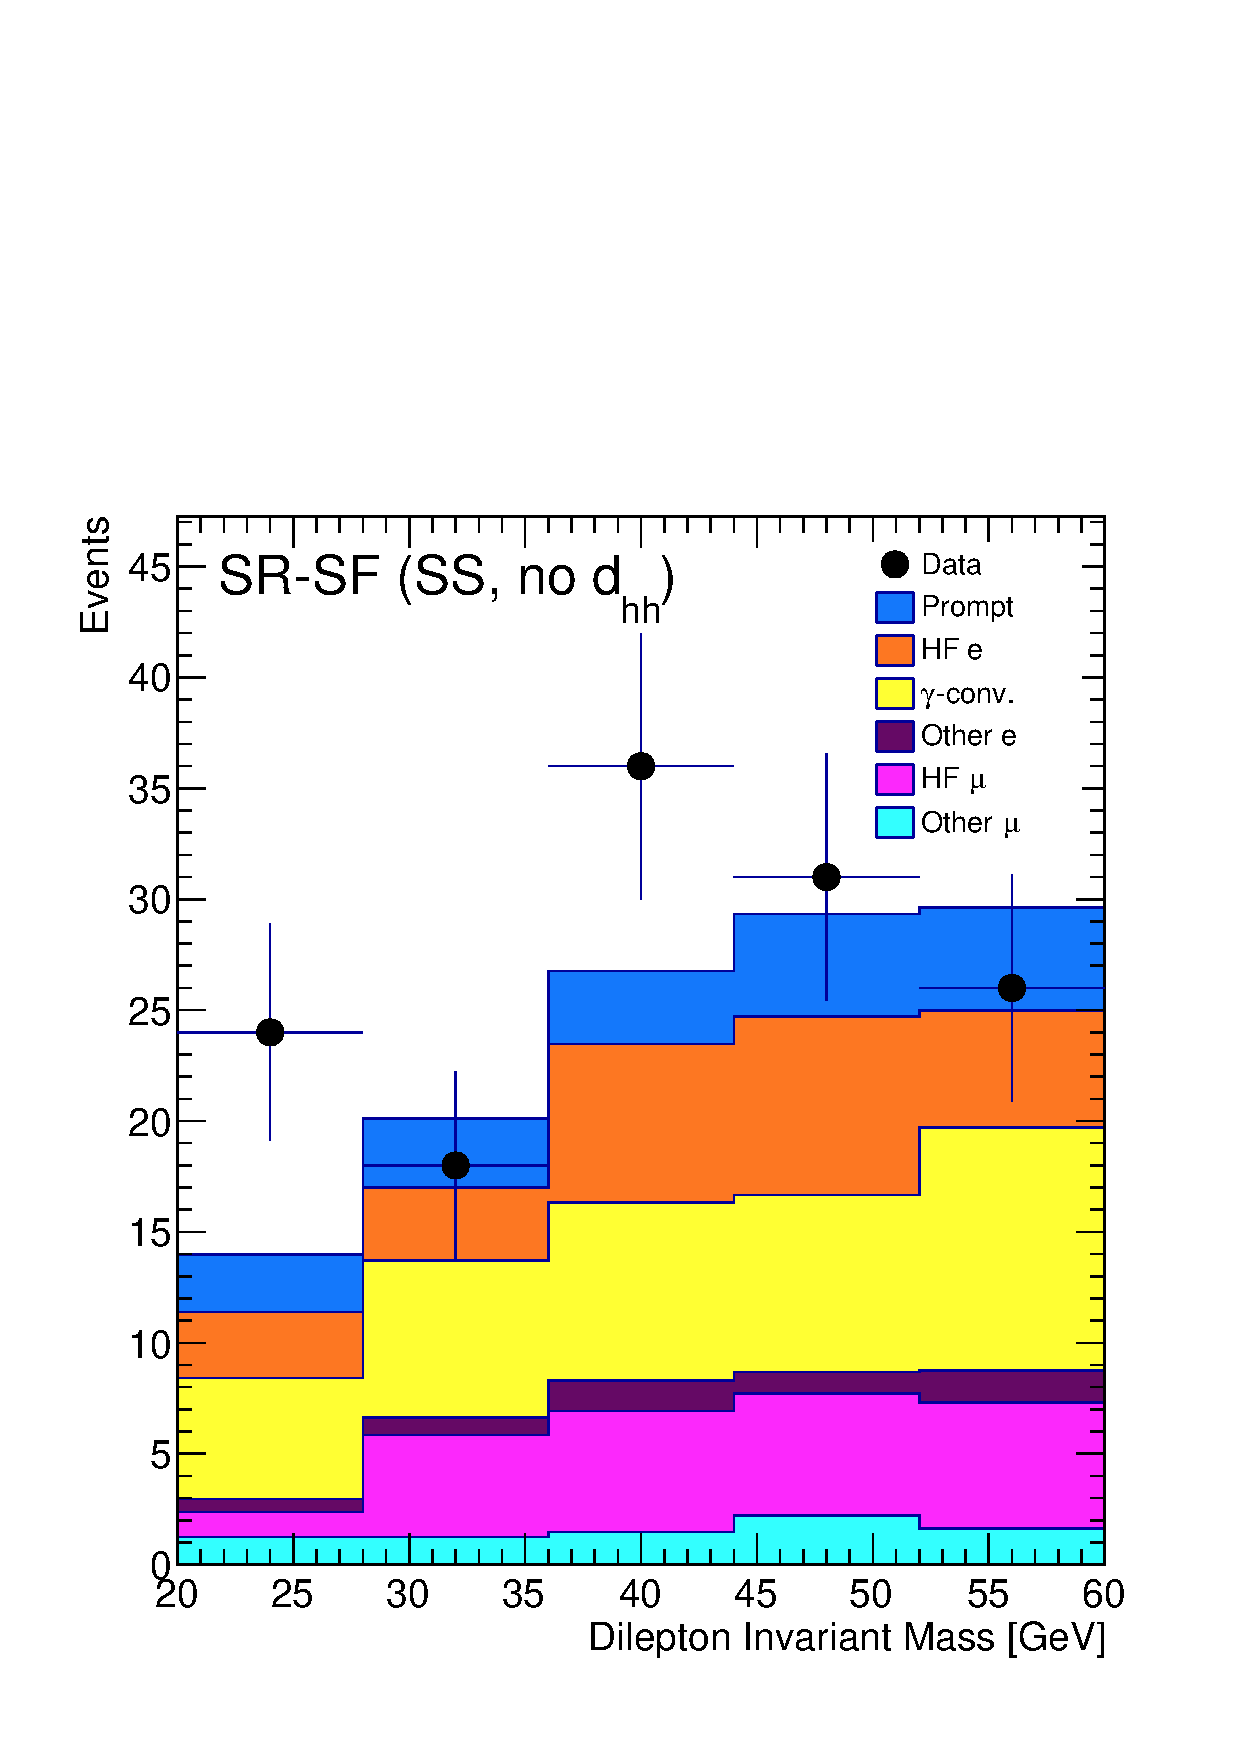
\includegraphics[width=0.45\textwidth]{figures/search_hh/bkg_estimate/fake/fake_val_sr_sf_ss_mll}
    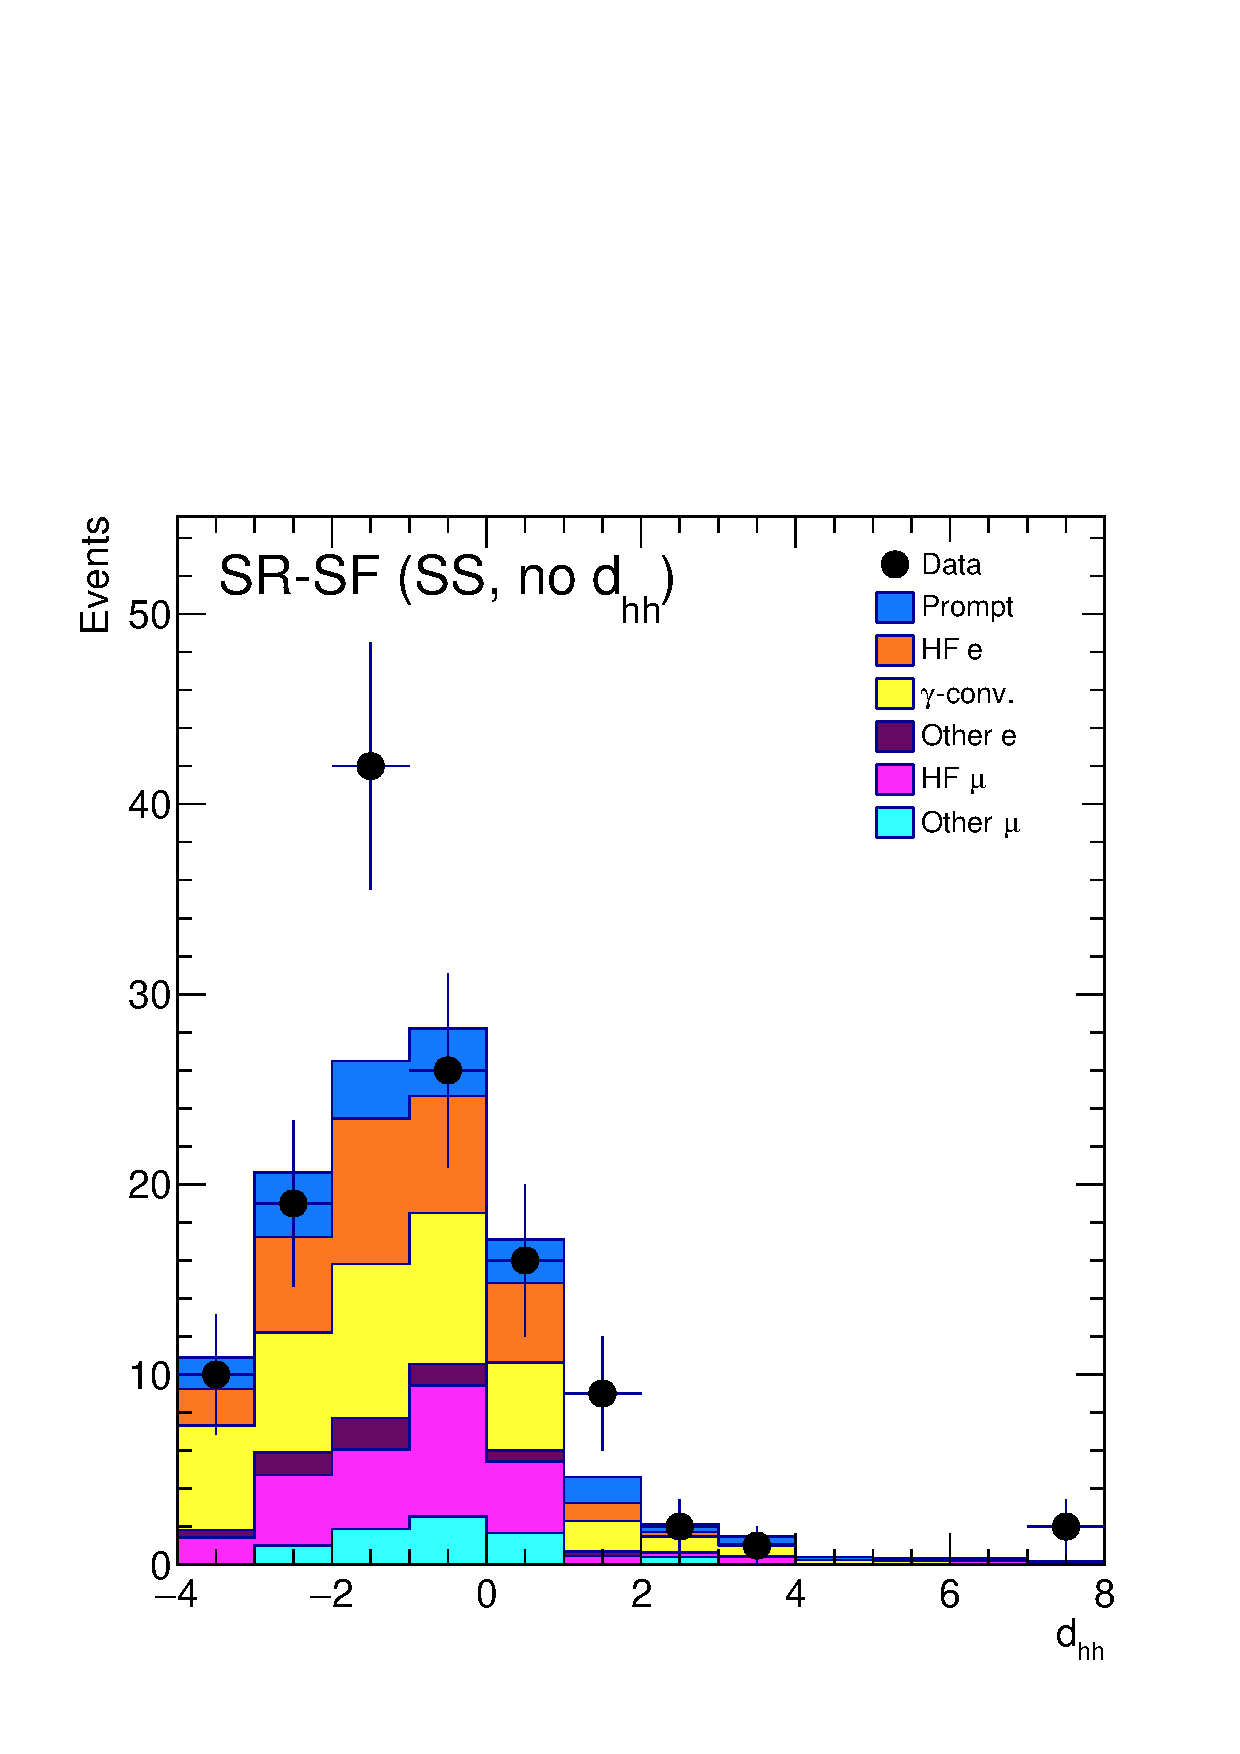
\includegraphics[width=0.45\textwidth]{figures/search_hh/bkg_estimate/fake/fake_val_sr_sf_ss_NN_d_hh}
    \caption{
        Data and MC distributions in the same-sign SR-SF selection with the $d_{hh}$ requirement removed.
        The non-prompt MC is broken into the categories described in the text.
        \textbf{\textit{top-left}}: Leading lepton $p_{T}$, \textbf{\textit{top-right}}: Sub-leading lepton $p_{T}$,
        \textbf{\textit{bottom-left}}: dilepton invariant mass, and \textbf{\textit{bottom-right}}: $d_{hh}$.
    }
    \label{fig:fake_val_srsf}
    \end{center}
\end{figure}

\begin{figure}[!htb]
    \begin{center}
    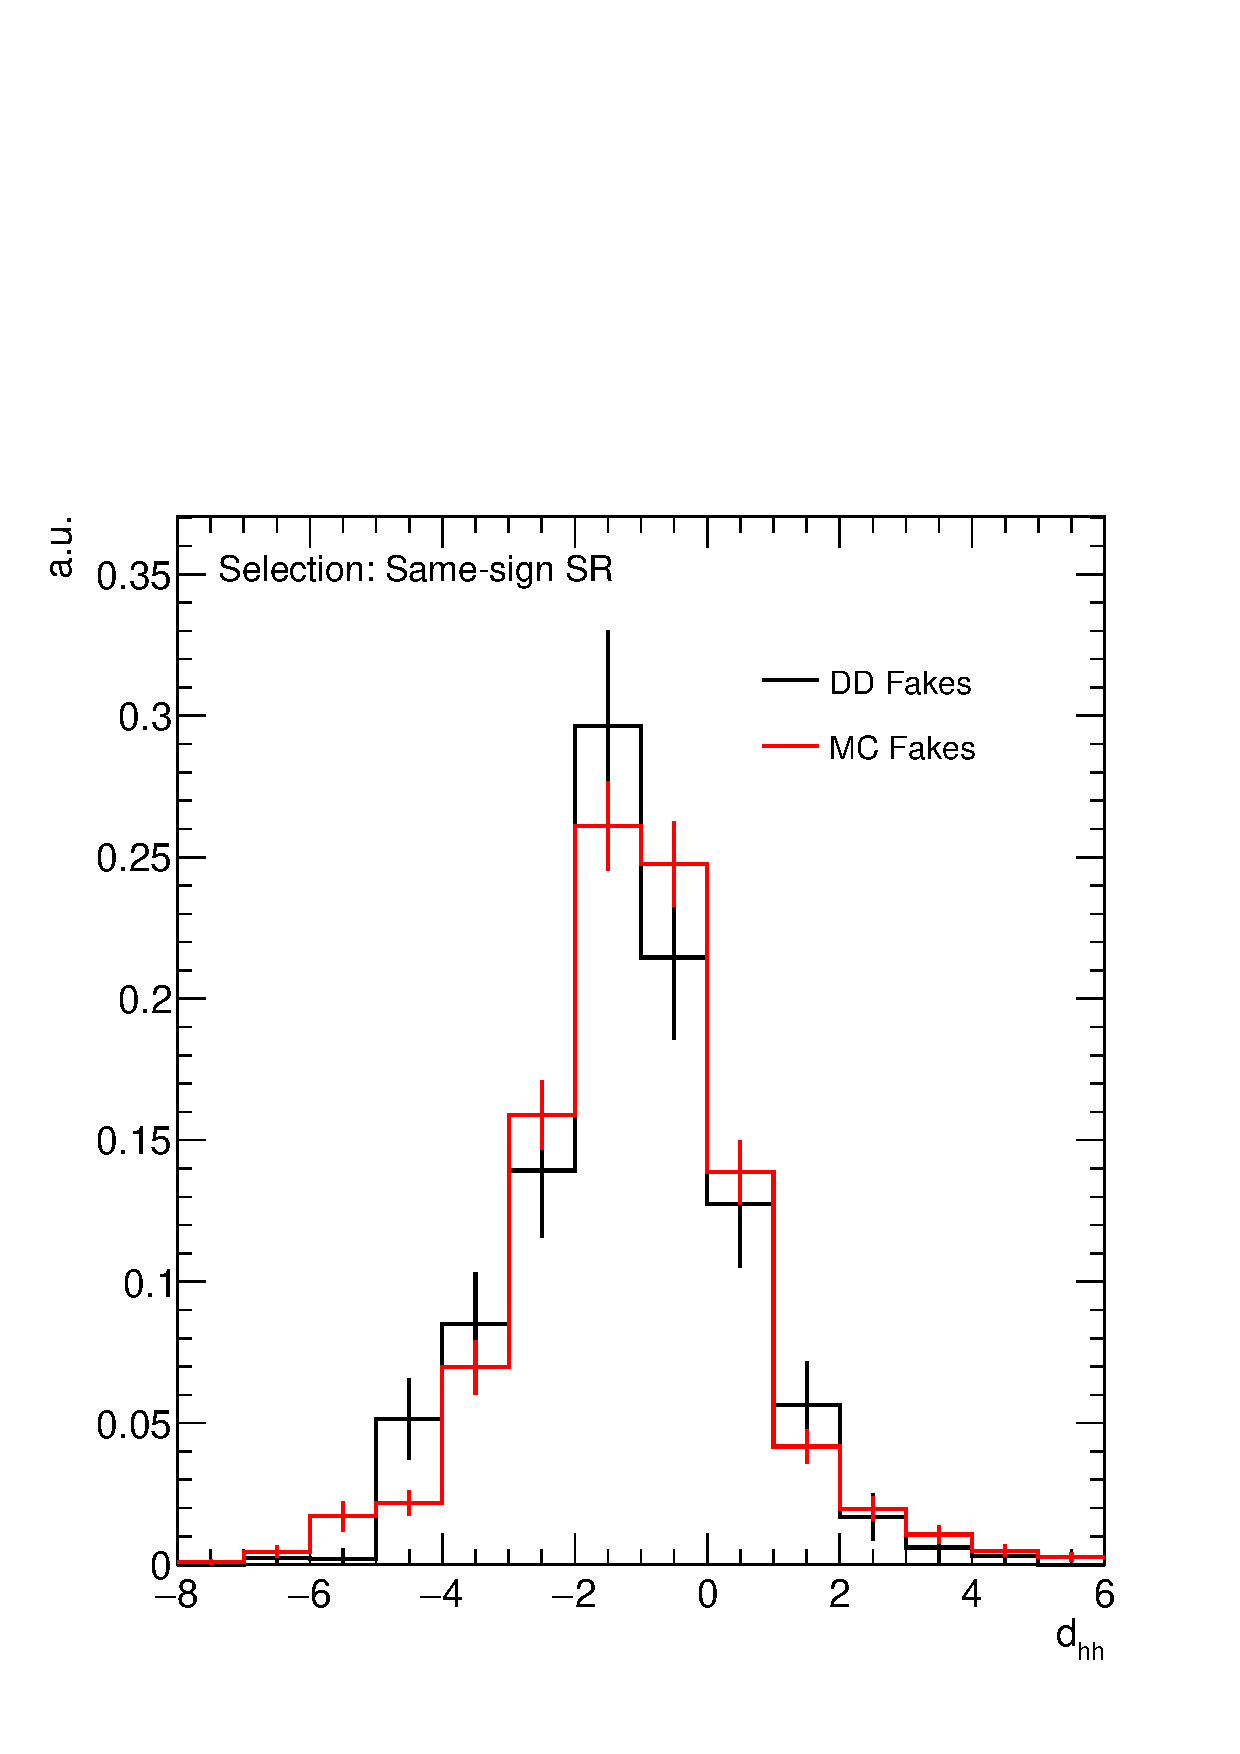
\includegraphics[width=0.45\textwidth]{figures/search_hh/bkg_estimate/fake/fake_shape_NN_d_hh_sr_ss_out}
    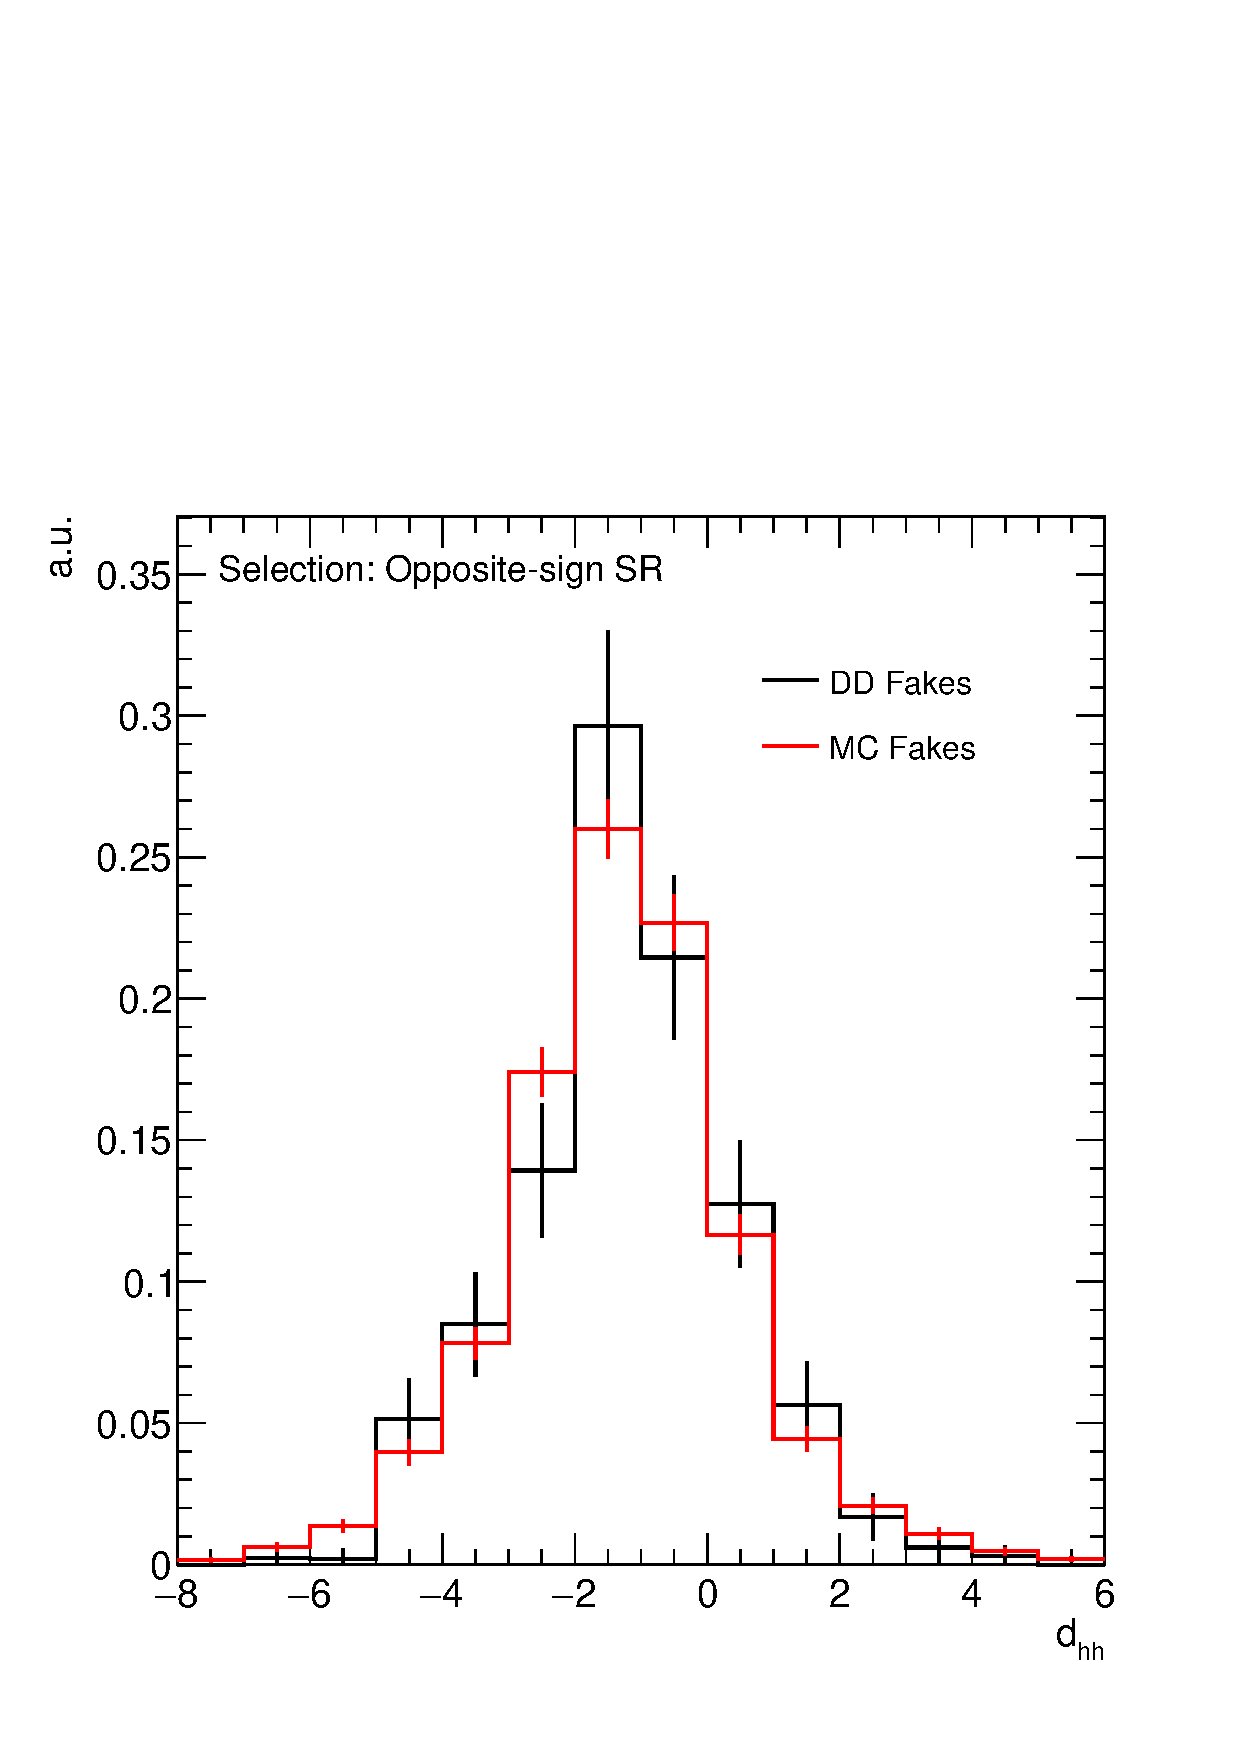
\includegraphics[width=0.45\textwidth]{figures/search_hh/bkg_estimate/fake/fake_shape_NN_d_hh_sr_os_out}
    \caption{
        Normalized \dhh distributions of the same-sign data with the real SM processes subtracted using MC (`DD Fakes') compared
            to the fake prediction using MC (`MC Fakes') in the SR selections inclusive of dilepton flavor (SF+DF).
            \textit{\textbf{Left}}: Same-sign lepton charge requirement.
            \textit{\textbf{Right}}: Opposite-sign lepton charge requirement.
    }
    \label{fig:fake_val_ss_os_shape}
    \end{center}
\end{figure}

For each region appearing in the analysis, a dedicated measurement of the quantities appearing in
Equation~\ref{eq:ss_extrap_dhh} is made, so that the fake estimate in every region can be obtained.
The measured values of all quantities needed for Equation~\ref{eq:ss_extrap_dhh} are reported
in Table~\ref{tab:hh_fake_quant}.
For each region, the $f^{SS \rightarrow OS}$ extrapolation factors are assessed for their dependence on
\dhh, to check whether or not any additional higher order correction to account for the change in the fake
composition as one extrapolates across the \dhh selection.
This is shown in Figure~\ref{fig:fake_val_os_ss_ratio} for SR-DF and SR-SF where it can be seen that there
is no statistically significant dependence of the $f^{SS \rightarrow OS}$ quantity on \dhh.
The same is found to hold for the CRs and VRs.
Figure~\ref{fig:fake_val_os_ss_ratio} also indicate the $\pm 20\%$ uncertainty taken on the $f^{SS \rightarrow OS}$
factors, defined as the typical spread of the $f^{SS \rightarrow OS}$ factors within each of the regions in 
the analysis.

In Tables~\ref{tab:fake_composition_srdf} and \ref{tab:fake_composition_srsf}, the breakdown of the sources
of fake leptons in the SS and OS versions of the analysis' signal regions, SR-DF and SR-SF, are presented
along with their associated $f^{SS \rightarrow OS}$ factors.
The single largest component of the fake background, in the OS regions, is due to conversion electrons.
However, considering both electrons and muons together, fake leptons are predominantly arising from
heavy flavor sources, such as in-flight semileptonic decays of $b$- and $c$-flavored hadrons.

\begin{figure}[!htb]
    \begin{center}
    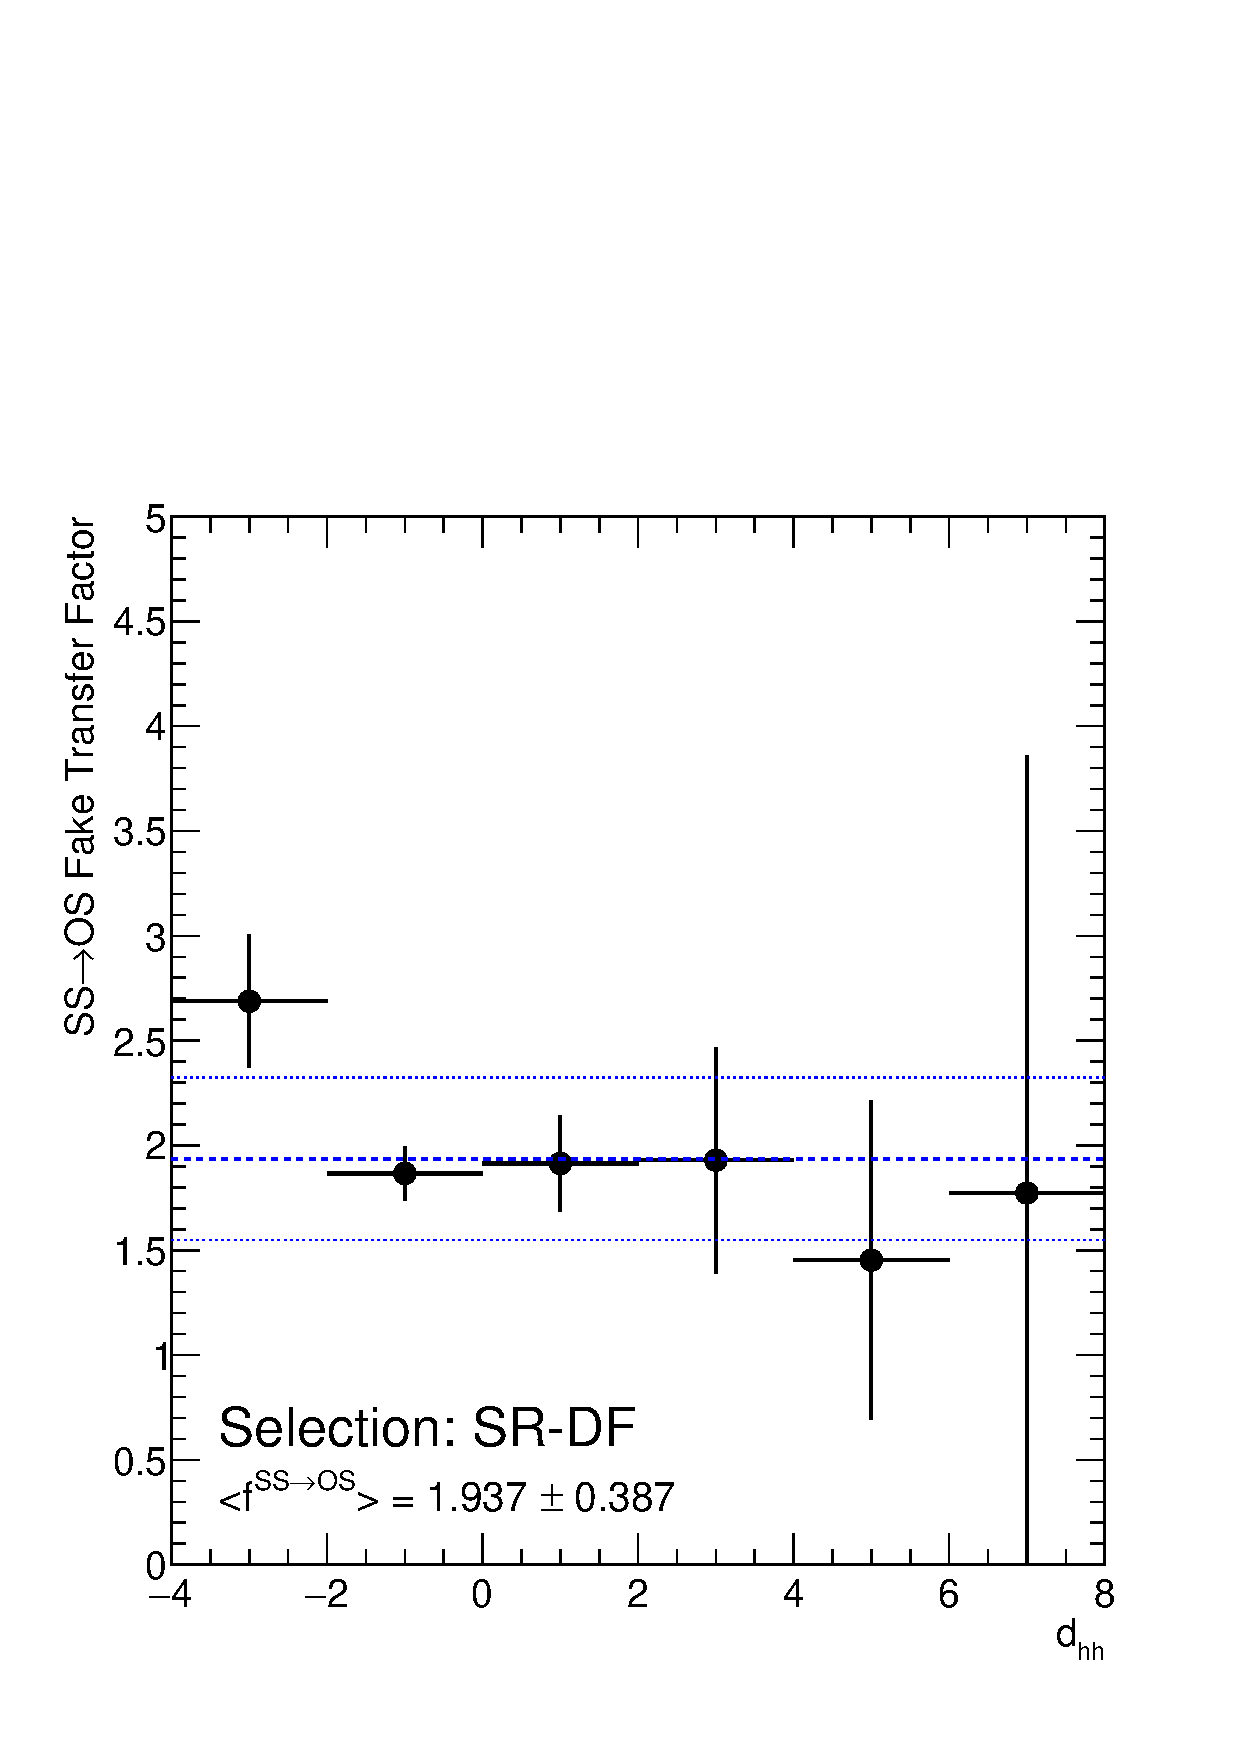
\includegraphics[width=0.45\textwidth]{figures/search_hh/bkg_estimate/fake/fake_val_os_ss_ratio_NN_d_hh_sr_df}
    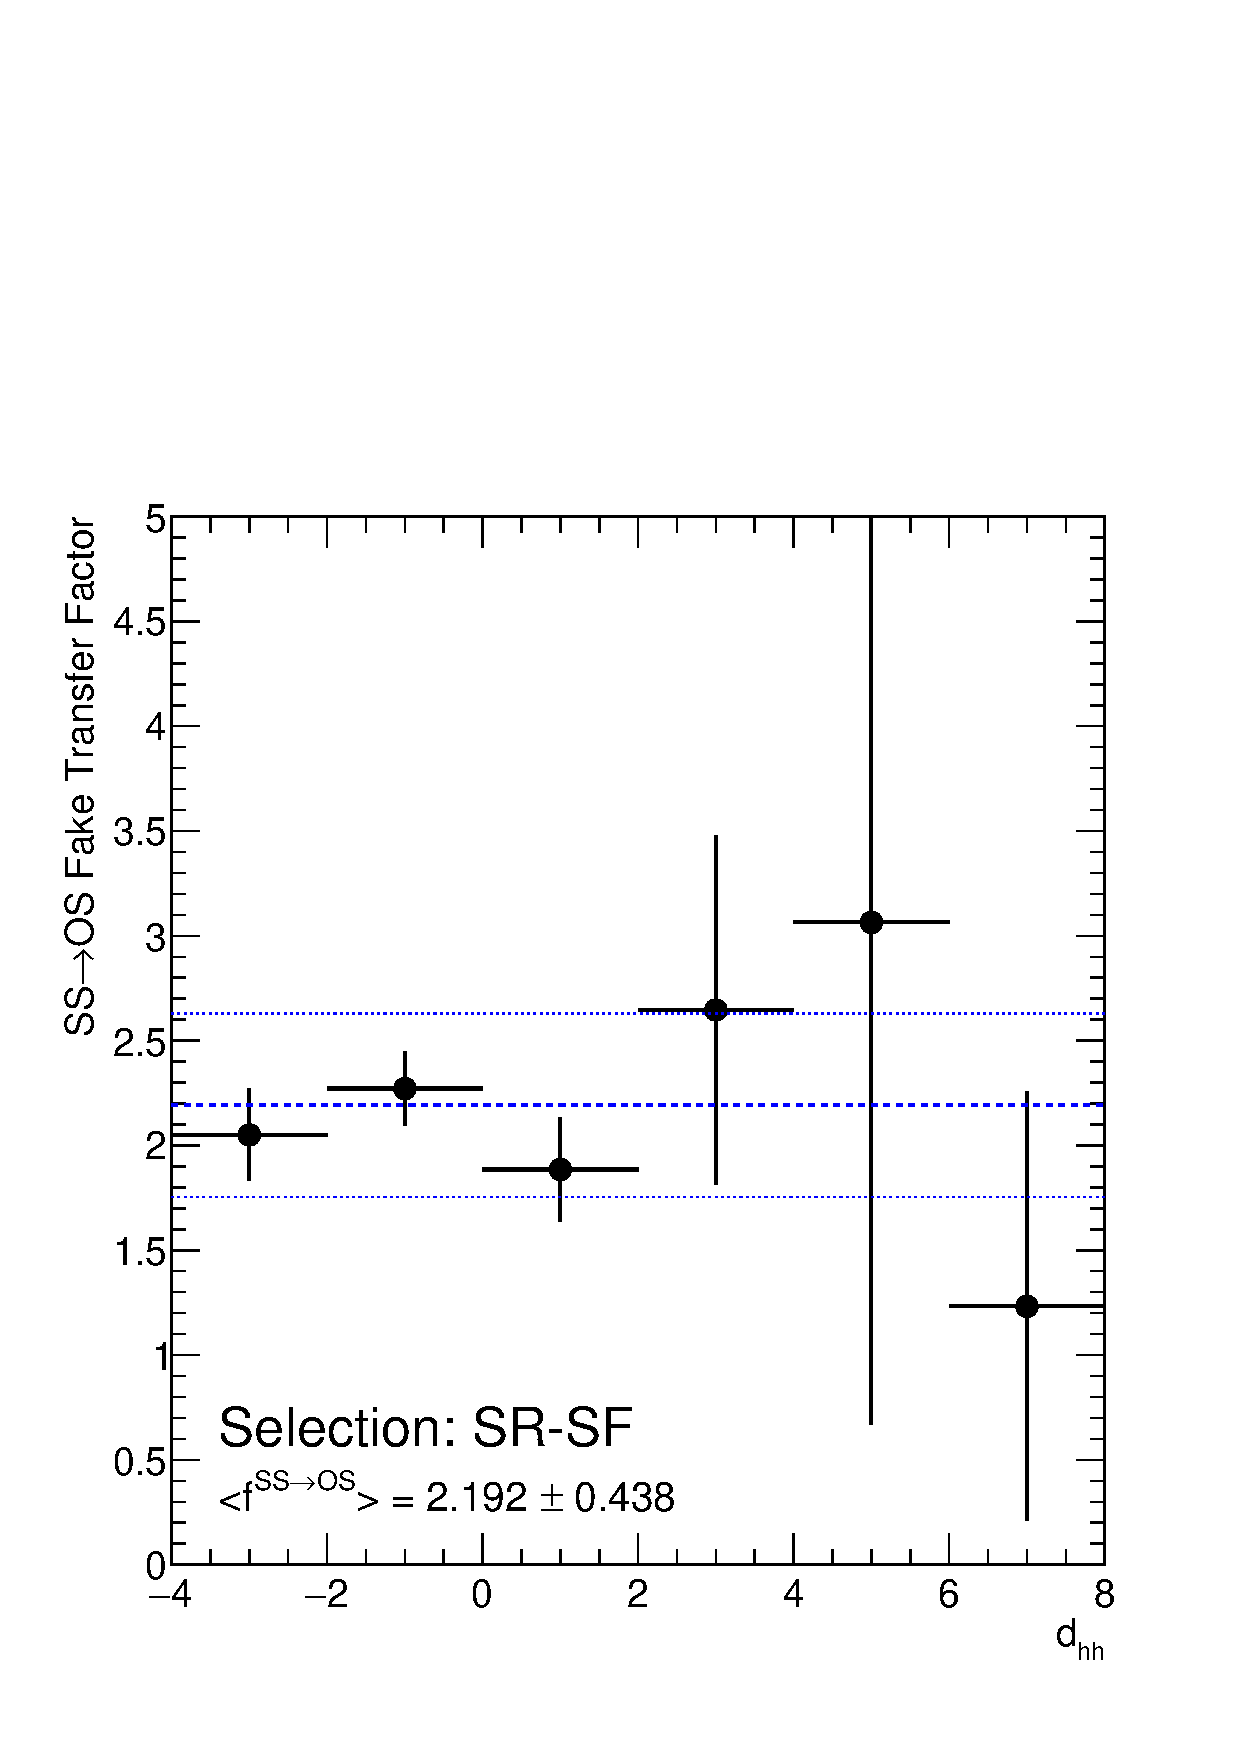
\includegraphics[width=0.45\textwidth]{figures/search_hh/bkg_estimate/fake/fake_val_os_ss_ratio_NN_d_hh_sr_sf}
    \caption{
        The $f^{SS \rightarrow OS}$ factors for SR-DF (\textit{\textbf{left}}) and SR-SF (\textit{\textbf{right}}) as a function
        of \dhh.
        The middle blue dashed lines are the average $f^{SS \rightarrow OS}$ across the \dhh range and the outer blue lines
        are the $\pm 20 \%$ shift about this average value.
    }
    \label{fig:fake_val_os_ss_ratio}
    \end{center}
\end{figure}

\begin{table}[!htb]
    \begin{center}
    \caption{
        Fake lepton sources based on truth level information in MC for the SS and OS different-flavor signal region selections,
        with inverted $d_{hh}$ selection. Uncertainties are statistical only.
        Shown also is the
        total MC fake, total MC prompt (non-fake), and Total MC (fake + non-fake) yields. The last row
        shows the observed number of events in each region. The right most column shows the
        ratio of the opposite-sign to same-sign yields for each of the fake sources.
    }
    \label{tab:fake_composition_srdf}
    \begin{tabular}{c | c c | c} % | c c}
    \hline
    \textbf{Source of Fake} & \textbf{SR-DF (SS, inverted $d_{hh}$)} & \textbf{SR-DF (OS, inverted $d_{hh}$)} & \textbf{OS/SS} \\
    \hline
    Heavy flavor $e$ & $35.70 \pm 2.67$ & $59.04 \pm 3.45$ & $1.65 \pm 0.16$ \\
    Conversion $e$ & $49.72 \pm 3.16$ & $98.65 \pm 4.43$ & $1.98 \pm 0.15$ \\
    Other $e$ & $6.16 \pm 1.11$ & $25.90 \pm 2.31$ & $4.20 \pm 0.85$ \\
    Heavy flavor $\mu$ & $23.00 \pm 2.46$ & $52.84 \pm 3.27$ & $2.29 \pm 0.28$ \\
    Other $\mu$ & $4.10 \pm 0.91$ & $13.77 \pm 1.67$ & $3.36 \pm 0.85$ \\
    \hdashline
    Total MC Fake & $118.67 \pm 5.02$ & $250.19 \pm 7.10$ & $2.10 \pm 0.11$ \\
    Total MC Prompt & $18.28 \pm 1.37$ & $16784.73 \pm 58.34$ & -\\
    \hline
    Total MC & $136.95 \pm 5.20$ & $17034.92 \pm 58.77$ & - \\
    Data & $158$ & $16720$ & - \\
    \hline
    \end{tabular}
    \end{center}
\end{table}

\begin{table}[!htb]
    \begin{center}
    \caption{
        Fake lepton sources based on truth level information in MC for the SS and OS same-flavor signal region selections,
        with inverted $d_{hh}$ selection. Uncertainties are statistical only.
        Shown also is the
        total MC fake, total MC prompt (non-fake), and Total MC (fake + non-fake) yields. The last row
        shows the observed number of events in each region. The right most column shows the
        ratio of the opposite-sign to same-sign yields for each of the fake sources.
    }
    \label{tab:fake_composition_srsf}
    \begin{tabular}{c | c c | c}
    \hline
    \textbf{Source of Fake} & \textbf{SR-SF (SS, inverted $d_{hh}$)} & \textbf{SR-SF (OS, inverted $d_{hh}$)} & \textbf{OS/SS} \\ 
    \hline
    Heavy flavor $e$ & $26.75 \pm 2.30$ & $44.37 \pm 2.97$ & $1.66 \pm 0.18$ \\
    Conversion $e$ & $39.11 \pm 2.88$ & $70.57 \pm 3.81$ & $1.80 \pm 0.16$ \\
    Other $e$ & $5.16 \pm 1.00$ & $16.04 \pm 1.75$ & $3.11 \pm 0.70$  \\
    Heavy flavor $\mu$ & $22.15 \pm 2.26$ & $66.12 \pm 3.70$ & $2.99 \pm 0.35$ \\
    Other $\mu$ & $7.82 \pm 1.31$ & $22.75 \pm 2.17$ & $2.91 \pm 0.56$ \\
    \hdashline
    Total MC Fake & $101.00 \pm 4.62$ & $219.87 \pm 6.70$ & $2.18 \pm 0.12$ \\
    Total MC Prompt & $18.00 \pm 1.28$ & $17903.42 \pm 64.27$ & - \\
    \hline
    Total MC & $119.00 \pm 4.80$ & $18123.29 \pm  64.62$ & - \\
    Data & $133$ & $17773$ & - \\
    \hline
    \end{tabular}
    \end{center}
\end{table}

\begin{table}[!htb]
    \begin{center}
    \caption{
        A summary of the quantities used in the determination of the fake contribution to the
        analysis regions and used as input to Equation~\ref{eq:ss_extrap_dhh}. The right-most
        column gives the actual fake estimate in each of the analysis regions. The uncertainty
        on $N^{\text{DD fake}}$ includes the effects of the $\pm20$\% uncertainty on
        $f^{SS \rightarrow OS}$, $\pm50$\% uncertainty taken on the prompt MC subtraction, and the
        uncertainty on $\varepsilon^{dhh}$.
    }
    \label{tab:hh_fake_quant}
    \begin{tabular}{c | c c c c || c}
    \hline
    \textbf{Region} & \textbf{$N_{\text{SS,data}}$} & \textbf{$N_{\text{SS,prompt MC}}$} & \textbf{$\varepsilon^{dhh}$} & \textbf{$f^{SS \rightarrow OS}$} & \textbf{$N^{\text{DD fake}} $} \\
    \hline
    CR-Top  & $799$ & $104.50 \pm 3.13$ & $ 0.0058 \pm 0.0010$ & $1.93 \pm 0.39$   & $7.79 \pm 3.34$ \\
    VR-Top  & $461$ & $54.49 \pm 1.89$  & $ 0.0066 \pm 0.0015$ & $1.83 \pm 0.37$   &  $4.91 \pm 2.14$ \\
    CR-Z+HF & $137$ & $40.66 \pm 3.73$  & $ 0.0347 \pm 0.0044$ & $2.73 \pm 0.55$   & $9.12 \pm 5.47$ \\
    VR-Z+HF & $110$ & $29.31 \pm 2.55$  & $ 0.0324 \pm 0.0054$ & $2.28 \pm 0.46$   &  $5.96 \pm 3.09$\\
    \hdashline
    SR-SF   & $133$ & $18.00 \pm 1.28$  & $ 0.0022 \pm 0.0013 $ & $2.10 \pm 0.42$  &  $0.55 \pm 0.39$\\
    SR-DF   & $158$ & $18.28 \pm 1.37$  & $ 0.0014 \pm 0.0010 $ &  $2.17 \pm 0.43$ &  $0.42 \pm 0.36$\\
    \hline
    \end{tabular}
    \end{center}
%    \end{footnotesize}
\end{table}

%%%%%%%%%%%%%%%%%%%%%%%%%%%%%%%%%%%%%%%%%%%%%%%%%%%%%%%%%%%%%%%%%%%%%%%%%%%%%%%%%%%
%%%%%%%%%%%%%%%%%%%%%%%%%%%%%%%%%%%%%%%%%%%%%%%%%%%%%%%%%%%%%%%%%%%%%%%%%%%%%%%%%%%
%%%%%%%%%%%%%%%%%%%%%%%%%%%%%%%%%%%%%%%%%%%%%%%%%%%%%%%%%%%%%%%%%%%%%%%%%%%%%%%%%%%
%
% BACKGROUND ONLY FIT
%
%%%%%%%%%%%%%%%%%%%%%%%%%%%%%%%%%%%%%%%%%%%%%%%%%%%%%%%%%%%%%%%%%%%%%%%%%%%%%%%%%%%
%%%%%%%%%%%%%%%%%%%%%%%%%%%%%%%%%%%%%%%%%%%%%%%%%%%%%%%%%%%%%%%%%%%%%%%%%%%%%%%%%%%
%%%%%%%%%%%%%%%%%%%%%%%%%%%%%%%%%%%%%%%%%%%%%%%%%%%%%%%%%%%%%%%%%%%%%%%%%%%%%%%%%%%

\FloatBarrier
\subsection{Background-only Fit}
\label{sec:hh_bkg_only}

As in Section~\ref{sec:stop_background_only}, we perform a background-only fit to
the observed data in the CRs defined in the present analysis.
The results are shown in terms of their impact on the post-fit predicted yields
in the CRs and VRs in Table~\ref{tab:hh_crvr_yields}.
The agreement observed between the post-fit MC and the observed data in the VRs
shows that the extrapolation is performing well.
The normalization correction factors derived in the fit for the Top and $Z$+heavy-flavor processes,
$\mu_{\text{Top}}$ and $\mu_{Z\text{+heavy-flavor}}$, respectively,
are reported in Table~\ref{tab:hh_norm_factors}.
The value for $\mu_{\text{Top}}$ is below one and indicates that the data prefers the combined \ttbar~and
single-top $Wt$ background estimate to be reduced, likely due to destructive interference effects
that are not taken into account in the MC prediction.
The rather large value of $\mu_{Z\text{+heavy-flavor}}$ is consistent with the measurements
reported by both ATLAS and CMS in Refs.~\cite{Chatrchyan:2013zja,Aad:2014dvb}, indicating that the MC
predictions of the $Z$+heavy-flavor process under-predict the cross-section in kinematic regions similar
to those being probed in the present analysis.
The value for $\mu_{Z\text{+heavy-flavor}}$ also happens to consistent with that found by the ATLAS search for the $hh \rightarrow \bbtautau$~\cite{HHBBTAUTAU},
which also has a dedicated measurement of a $Z$+heavy-flavor normalization correction. 

\begin{table}
\begin{center}
\caption{
Table showing the pre- and post-fit yields for the contributing MC background processes in the
Top and $Z$+heavy flavor control and validation regions.
The $Z$+heavy-flavor and $Z$+light-flavor backgrounds are separated into the high-$m_{\ell \ell}$
($m_{\ell \ell} > 60$ GeV) and low-$m_{\ell \ell}$ ($m_{\ell \ell} < 60$ GeV) components,
with the latter labelled as `Drell-Yan'.
The uncertainties on the yield estimates include all uncertainties discussed in Section \ref{sec:common_systematics}.
}
\label{tab:hh_crvr_yields}
\setlength{\tabcolsep}{0.0pc}
{\small
%%
\begin{tabular*}{\textwidth}{@{\extracolsep{\fill}}lrrrr}
\noalign{\smallskip}\hline\noalign{\smallskip}
\textbf{Region}          & CR-Top            & CR-Z+HF            & VR-Top            & VR-Z+HF              \\[-0.05cm]
\noalign{\smallskip}\hline\noalign{\smallskip}
%%
 Observed Data         & $108$              & $852$              & $171$              & $157$                    \\
\noalign{\smallskip}\hline\noalign{\smallskip}
%%
 Post-fit Total SM          & $107.99 \pm 10.39$          & $851.94 \pm 29.19$          & $161.75 \pm 10.30$          & $147.07 \pm 10.54$              \\
\noalign{\smallskip}\hline\noalign{\smallskip}

        Post-fit \ttbar          & $55.32 \pm 6.86$          & $40.57 \pm 5.50$          & $45.96 \pm 6.00$          & $59.32 \pm 8.94$              \\
%%
        Post-fit Single-top $Wt$          & $36.34 \pm 4.69$          & $14.63 \pm 2.13$          & $31.24 \pm 4.30$          & $11.58 \pm 1.80$              \\
%%
        Post-fit $\ttbar+V$          & $2.22 \pm 0.23$          & $27.60 \pm 2.41$          & $4.49 \pm 0.42$          & $3.20 \pm 0.28$              \\
%%
        Post-fit $Z$+heavy-flavor          & $3.22 \pm 0.47$          & $686.48 \pm 32.95$          & $26.76 \pm 1.59$          & $60.39 \pm 3.56$              \\
%%
        Post-fit $Z$+light-flavor          & $0.23 \pm 0.08$          & $27.10 \pm 8.91$          & $1.37 \pm 0.51$          & $2.49 \pm 0.77$              \\
%%
        Post-fit Diboson          & $0.72 \pm 0.12$          & $0.75 \pm 0.45$          & $0.27 \pm 0.07$          & $0.20 \pm 0.05$              \\
%%
        Post-fit Single-higgs          & $2.23 \pm 0.79$          & $45.76 \pm 3.60$          & $0.81 \pm 0.09$          & $4.00 \pm 0.80$              \\
%%
        Post-fit Drell-Yan heavy-flavor          & $0.00 \pm 0.00$          & $0.00 \pm 0.00$          & $43.57 \pm 2.43$          & $0.00 \pm 0.00$              \\
%%
        Post-fit Drell-Yan heavy-flavor         & $0.00 \pm 0.00$          & $0.00 \pm 0.00$          & $2.42 \pm 1.06$          & $0.00 \pm 0.00$              \\
%%
        Post-fit Fakes          & $7.71 \pm 3.29$          & $9.03 \pm 5.38$          & $4.86 \pm 2.09$          & $5.89 \pm 3.06$              \\


 \noalign{\smallskip}\hline\noalign{\smallskip}
%%
Total SM               & $131.38 \pm 6.68$          & $685.45 \pm 15.41$          & $163.63 \pm 6.25$          & $149.89 \pm 8.75$              \\
\noalign{\smallskip}\hline\noalign{\smallskip}
%%
        \ttbar          & $69.95 \pm 4.45$          & $51.30 \pm 3.88$          & $58.11 \pm 3.79$          & $75.00 \pm 7.65$              \\
%%
        Single-top $Wt$          & $45.97 \pm 2.71$          & $18.51 \pm 1.50$          & $39.51 \pm 2.60$          & $14.65 \pm 1.45$              \\
%%
        $\ttbar+V$          & $2.22 \pm 0.23$          & $27.59 \pm 2.42$          & $4.49 \pm 0.42$          & $3.20 \pm 0.28$              \\
%%
        $Z$+heavy-flavor          & $2.37 \pm 0.33$          & $505.44 \pm 5.00$          & $19.70 \pm 0.65$          & $44.46 \pm 1.51$              \\
%%
        $Z$+light-flavor          & $0.23 \pm 0.08$          & $27.10 \pm 8.97$          & $1.37 \pm 0.52$          & $2.49 \pm 0.77$              \\
%%
        Diboson          & $0.72 \pm 0.12$          & $0.75 \pm 0.45$          & $0.27 \pm 0.07$          & $0.20 \pm 0.05$              \\
%%
        Single-higgs          & $2.23 \pm 0.79$          & $45.74 \pm 3.63$          & $0.81 \pm 0.09$          & $4.00 \pm 0.80$              \\
%%
        Drell-Yan heavy-flavor          & $0.00 \pm 0.00$          & $0.00 \pm 0.00$          & $32.08 \pm 0.83$          & $0.00 \pm 0.00$              \\
%%
        Drell-Yan light-flavor          & $0.00 \pm 0.00$          & $0.00 \pm 0.00$          & $2.42 \pm 1.07$          & $0.00 \pm 0.00$              \\
%%
        Fakes          & $7.71 \pm 3.29$          & $9.03 \pm 5.38$          & $4.86 \pm 2.09$          & $5.89 \pm 3.06$              \\


\noalign{\smallskip}\hline\noalign{\smallskip}
\end{tabular*}
%%%
}
\end{center}
\end{table}


\begin{table}[!htb]
    \begin{center}
        \caption{
            Normalization correction factors derived for the Top and $Z$+heavy-flavor background
            processes in the search targeting the dilepton $hh \rightarrow \bbww$ signal process.
        }
        \label{tab:hh_norm_factors}
        \begin{tabular}{l | c}
        \hline
        \hline
            $\mu_{\text{Top}}$ & $0.79 \pm 0.10$ \\
            $\mu_{Z\text{+heavy-flavor}}$ & $1.35 \pm 0.07$ \\
        \hline
        \hline
        \end{tabular}
    \end{center}
\end{table}
